\documentclass[11pt,a4paper]{amsart}
\usepackage[T1]{fontenc}
\usepackage{lmodern,microtype}
\usepackage[margin=28mm,headheight=14pt]{geometry}
\usepackage{amsmath,amssymb,mathtools,mathrsfs,booktabs,array,enumitem}
\usepackage{xcolor,tikz}
\usetikzlibrary{arrows.meta,positioning,calc}
\usepackage[colorlinks=true,linkcolor=blue!45!black,citecolor=blue!45!black,urlcolor=blue!45!black]{hyperref}
\hypersetup{pdftitle={Programming Nonlinear Magnetic Response with Twelve Mechanical Modes},pdfauthor={Harjas Sandhu}}
\setlength{\emergencystretch}{2em}
\setlist[enumerate]{leftmargin=*,itemsep=3pt,topsep=5pt}
\setlist[itemize]{leftmargin=*,itemsep=3pt,topsep=5pt}
\newtheorem{theorem}{Theorem}[section]
\newtheorem{proposition}[theorem]{Proposition}
\newtheorem{lemma}[theorem]{Lemma}
\newtheorem{corollary}[theorem]{Corollary}
\theoremstyle{definition}
\newtheorem{definition}[theorem]{Definition}
\newtheorem{example}[theorem]{Example}
\theoremstyle{remark}
\newtheorem{remark}[theorem]{Remark}
\numberwithin{equation}{section}
\newcommand{\T}{\mathbb T}
\newcommand{\R}{\mathbb R}
\newcommand{\Z}{\mathbb Z}
\newcommand{\Q}{\mathbb Q}
\newcommand{\N}{\mathbb N}
\newcommand{\PP}{\mathbb P}
\newcommand{\Bcal}{\mathcal B}
\newcommand{\Ccal}{\mathcal C}
\newcommand{\Mcal}{\mathcal M}
\newcommand{\Hcal}{\mathcal H}
\newcommand{\Ecal}{\mathcal E}
\newcommand{\Gcal}{\mathcal G}
\newcommand{\Dcal}{\mathcal D}
\newcommand{\ip}[2]{\langle #1,#2\rangle}
\newcommand{\norm}[1]{\lVert #1\rVert}
\newcommand{\abs}[1]{\lvert #1\rvert}
\newcommand{\mean}[1]{\langle #1\rangle}
\newcommand{\diver}{\operatorname{div}}
\newcommand{\curl}{\operatorname{curl}}
\newcommand{\supp}{\operatorname{supp}}
\newcommand{\esssup}{\operatorname*{ess\,sup}}
\newcommand{\push}[1]{(#1)_*}
\DeclareMathOperator{\Id}{Id}
\DeclareMathOperator{\Rea}{Re}
\DeclareMathOperator{\diag}{diag}
\title[Nonlinear magnetic response]{Programming Nonlinear Magnetic Response\\ with Twelve Mechanical Modes}
\author{Harjas Sandhu}
\address{The University of Queensland}
\email{harjas.sandhu@student.uq.edu.au}
\date{12 November 2026}
\subjclass[2020]{35Q35, 35Q60, 93B05, 93C73, 76W05}
\keywords{Resistive magnetohydrodynamics, nonlinear response, ensemble control, finite-dimensional forcing, unknown diffusivity}
\begin{document}
\begin{abstract}
We study prescribed finite-time responses to the unobserved conserved magnetic
mean in the three-dimensional viscous, resistive magnetohydrodynamic equations.
The control acts only in the momentum equation, through twelve fixed fundamental
Fourier shear fields. A deterministic compiler programs an even polynomial
velocity response and an odd polynomial magnetic fluctuation of that mean.
Its single open-loop force is uniform over a bounded unknown preparation,
independent positive spatially constant diffusivity histories with supplied
Lipschitz bounds, sufficiently small absolute disturbances, and every
energy-admissible weak realization. The degree, coefficient lists and Fourier
supports are variable input; physical and binary costs have universal
polynomial bounds in the numerical parameters and complete description length.
The construction first evaluates odd magnetic registers, loads one collinear
packet batch, writes a small even velocity, and amplifies it while preserving
the magnetic output. A dyadic return word controls amplification on the whole
error space; an inverse-carrier estimate controls the complete unwanted packet
output. The result is an endpoint theorem for globally supported periodic
forcing. It supplies no hardware, affordability or autonomous computation claim.
\end{abstract}

\maketitle
\raggedbottom
\section{Introduction}
Suppose a conducting fluid contains an unknown magnetic flux. A force can be
chosen in advance, but neither the flux nor the transport coefficients can be
measured during the experiment. Can this one force make the final velocity and
magnetic field depend on that flux in a prescribed nonlinear way? The problem
is different from steering one known preparation to one known state: the same
physical experiment must implement an entire response map.

The input is the conserved magnetic mean $H$. Its normalized value $h=H/M$
belongs to the unit ball by the preparation bound. The requested endpoint is
\begin{equation}\label{eq:intro-endpoint}
 (u,B)=\bigl(U(x,h),\ H+Z(x,h)\bigr),\qquad h=H/M,
\end{equation}
up to a supplied absolute error. The coefficient fields of $U,Z$ are
solenoidal and mean zero. Magnetic sign symmetry requires $U$ to be even and
$Z$ odd. Their polynomial degree and complete rational Fourier lists are
variable input. No invertibility, monotonicity, separability or small
nonlinear-part assumption is imposed.

\subsection{Contribution and its relation to earlier control results}
The new operation is the simultaneous nonlinear joint response
\eqref{eq:intro-endpoint}, with a universal resource exponent as the degree
grows, under unknown preparation and independent time-dependent diffusivities.
Its foundations are a fixed-depth linear magnetic assembly and memory-preserving
mechanical operations. Its additional steps are actual magnetic register
arithmetic, an amplifier bounded on every error mode, and one collinear
readout whose complete higher output decreases with its carrier frequency.
These steps are proved separately before they are composed. The linear
construction appears explicitly in Sections~\ref{sec:algebra}--\ref{sec:heat};
it is recovered with its original Sobolev input class in
Corollary~\ref{cor:linear-recovery}.

Finite-mode control, saturation, return methods and reversible arithmetic
are established tools. The twelve shear directions used here already form a
saturating space in Nersesyan's work
\cite[Theorem~4.1 and Proposition~4.3]{Nersesyan2015}.
The forcing-direction method of Agrachev--Sarychev \cite{AS2005} and its
three-dimensional developments \cite{Shirikyan2006,Nersesyan2015,Nersesyan21}
provide the geometric background. Qualitative saturation does not by itself
give a coefficient-blind force, a stable variable-depth register machine, or
the numerical resource bounds required here. The explicit common-control
construction in \cite{Common} is the quantitative control foundation.

Earlier MHD results also have distinct and substantial scopes. Galan
\cite[Theorem~2.1]{Galan2011} treats approximate torus controllability with
controls in both equations. Rissel \cite[Theorem~1.2]{Rissel} treats known
smooth two-dimensional ideal data with two interior controls and a magnetic
cohomology condition. Rissel--Wang \cite[Theorems~1.2 and~1.5]{RisselWang}
establish global approximate boundary control under specified slip conditions;
their general theorem allows additional induction terms. Momentum-only
control is itself an established possibility: Tao--Yao--Yin \cite{TaoYaoYin}
prove local trajectory controllability in a bounded two-dimensional domain,
under their boundary and reference-trajectory hypotheses. None of these
statements is used as an unknown-ensemble response or polynomial-resource
theorem. Appendix~\ref{app:imports} records the exact imports actually needed.

The separate seed operation in \cite{Seed} starts with a prepared nonzero
magnetic seed and produces a specified field. Programming a response to an
unknown conserved mean is a different task. In particular, zero mean does
not mean that the initial magnetic field vanishes. The endpoint here requests
zero magnetic output when $H=0$; it does not assert that mechanical control
cannot act on a nonzero mean-zero seed.

\subsection{Conceptual overview: compute first, read once}
A magnetic register is a finite group of oscillatory Fourier coefficients
whose amplitudes hold unknown odd functions of $h$. A force can route and
multiply those amplitudes without measuring them. Logical arithmetic alone
does not make a register physical: unwanted modes, diffusion, induced
velocity and historical errors must be controlled in the actual equations.

The even velocity target has the exact decomposition
$U=U_0+\sum_jh_jR_j$ with odd $R_j$ and no division by $h_j$.
Thus all nonlinear arithmetic can be performed magnetically while velocity
is still disposable. The computation returns to the same finite code space
after every assignment, using genuine smoothing and an actual mechanical
restore. Nonexpansive whole-register assignments keep old coefficient errors
from accumulating exponentially with the polynomial degree.

The final conversion to velocity is made once. All packet carriers point in
one common direction. Solenoidality then removes the large carrier factor
from the first nonlinear interaction. After physical high-frequency clearing,
the entire higher output is inverse-carrier small. A bounded dyadic return
word first defines a small preconditioned target and then amplifies the
written velocity. The inverse word has polynomial gain on the \emph{whole}
mean-zero error space, including modes absent from the target. It returns
ideal magnetic transport to the identity. Finally a known velocity increment
adds $U_0$ while retaining both unknown fields.

\begin{center}
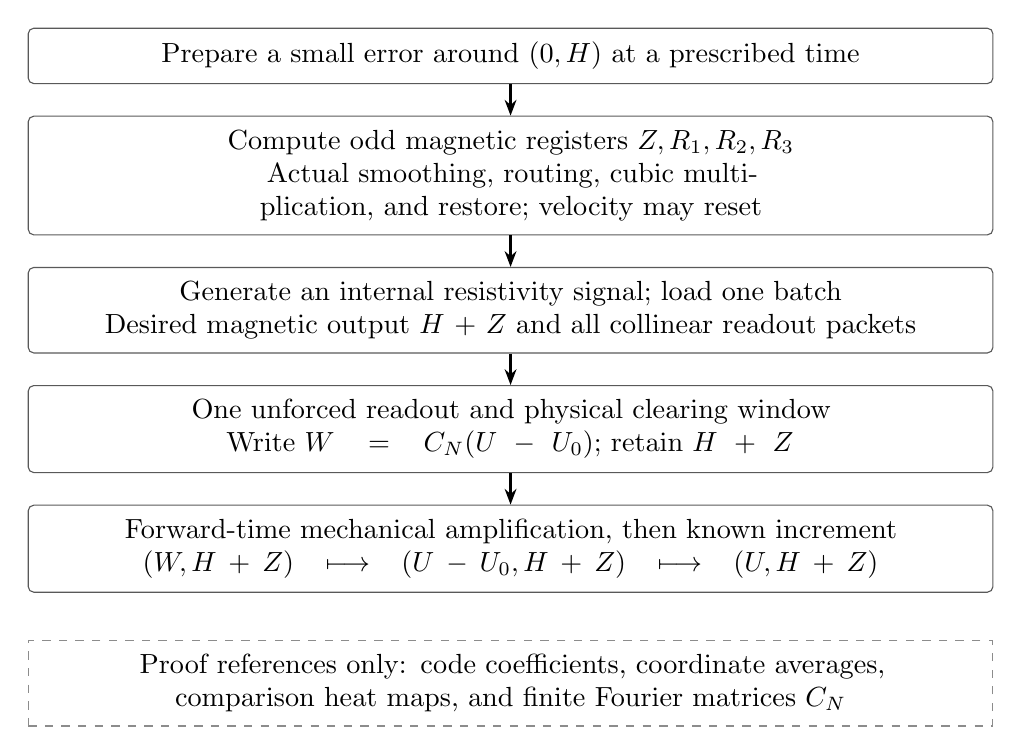
\begin{tikzpicture}[node distance=4mm,
 box/.style={draw=black!65,rounded corners=2pt,text width=11.9cm,
             align=center,inner sep=5pt},
 ref/.style={draw=black!45,dashed,text width=11.9cm,align=center,inner sep=5pt},
 arr/.style={-{Stealth[length=2mm]},thick}]
\node[box] (p) {Prepare a small error around $(0,H)$ at a prescribed time};
\node[box,below=of p] (a) {Compute odd magnetic registers $Z,R_1,R_2,R_3$\\
 Actual smoothing, routing, cubic multiplication, and restore; velocity may reset};
\node[box,below=of a] (l) {Generate an internal resistivity signal; load one batch\\
 Desired magnetic output $H+Z$ and all collinear readout packets};
\node[box,below=of l] (r) {One unforced readout and physical clearing window\\
 Write $W=C_N(U-U_0)$; retain $H+Z$};
\node[box,below=of r] (g) {Forward-time mechanical amplification, then known increment\\
 $(W,H+Z)\ \longmapsto\ (U-U_0,H+Z)\ \longmapsto\ (U,H+Z)$};
\node[ref,below=6mm of g] (c) {Proof references only: code coefficients, coordinate averages,\\
 comparison heat maps, and finite Fourier matrices $C_N$};
\draw[arr](p)--(a);\draw[arr](a)--(l);\draw[arr](l)--(r);\draw[arr](r)--(g);
\end{tikzpicture}
\end{center}
Solid boxes are executed by momentum forcing and unforced evolution. The
dashed box lists mathematical descriptions used to analyze them. In
particular, neither a coordinate average nor an inverse heat operator is
applied to the physical state. The preconditioner acts on the \emph{known
target coefficients} in the compiler. Its reverse effect on the fluid is
implemented by actual mechanical words.

\subsection{How to read the proof}
Theorem~\ref{thm:nonlinear} states the complete input and realization
quantifiers. Section~\ref{sec:arithmetic} isolates the stable finite
arithmetic. Sections~\ref{sec:algebra}--\ref{sec:heat} develop the reusable
linear, geometric, memory and heat foundation. Sections~\ref{sec:registers},
\ref{sec:amplifier} and~\ref{sec:readout} supply the new physical operations.
Section~\ref{sec:nonlinear-compiler} fixes their noncircular parameter order
and resource ledger. Long estimates are placed in the appendices.

\begin{center}\small
\begin{tabular}{@{}p{.22\linewidth}p{.70\linewidth}@{}}\toprule
Notation & Meaning\\\midrule
$H$, $h=H/M$ & Conserved unknown mean and normalized logical input\\
$U,Z,R_j$ & Even velocity target, odd magnetic fluctuation, odd cofactors\\
$D,N,F$ & Polynomial degree, retained output band, logical code frequency bound\\
$\mathscr C$, $T_i(\phi)$ & Normalized curl and ideal differential magnetic gate\\
$\mu$ & $\min(\nu_-,\rho_-)$, a supplied positive lower diffusivity bound\\
$Q$, $\sigma$ & Final readout carrier and its critical packet budget\\
$g$, $G_a$ & Preconditioning gain and whole-space amplification bound\\
$P$ & Computably generated positive-coefficient polynomial envelope\\
\bottomrule\end{tabular}\end{center}
The symbols $h$ and $H$ denote flux variables. Local durations are written
$d_{\mathrm c},d,\ell,T$ or as explicitly subscripted clocks. The resource
polynomial can have very large fixed constants and powers. This is a
finite-time PDE control result, not a cost advantage for a physical processor.

\section{The model and the response theorems}\label{sec:model}
Let $\T^3=\R^3/\Z^3$ have volume one and put $\kappa=2\pi$.
For a vector field, $\widehat v(k)=\int_{\T^3}v(x)e^{-i\kappa k\cdot x}\,dx$ and
\[
 \norm v_{H^s}^2=\sum_{k\in\Z^3}(1+\kappa^2|k|^2)^s|\widehat v(k)|^2.
\]
Matrix norms sum these squared norms over the entries. The joint norm
$\norm{(u,B)}_{\Hcal^s}^2=\norm u_{H^s}^2+\norm B_{H^s}^2$ is inhomogeneous:
constant magnetic fields are included. Let $\PP_k=I-k\otimes k/|k|^2$ for
$k\ne0$ and $\PP_0=I$. On solenoidal fields set
\[
 \Bcal(v,z)=\PP[(v\cdot\nabla)z],\quad
 L_vz=\Bcal(v,z)+\Bcal(z,v),\quad
 \Ccal_vb=(b\cdot\nabla)v-(v\cdot\nabla)b.
\]
The sign convention for $\Ccal$ makes the ideal induction map a vector
pushforward. It is the negative of the convention for $C$ in \cite{Common}.
The physical equations are
\begin{equation}\label{eq:mhd}
 \begin{aligned}
 u_t&=\nu(t)\Delta u-\Bcal(u,u)+\Bcal(B,B)+f+h_u,\\
 B_t&=\rho(t)\Delta B+\Ccal_uB+h_B,\\
 \diver u&=\diver B=0,\qquad \mean u=0.
 \end{aligned}
\end{equation}
Only the momentum force is chosen, and it always belongs to
\begin{equation}\label{eq:actuators}
 \Ecal=\operatorname{span}_{\R}
 \{e_i\cos(\kappa x_j),\ e_i\sin(\kappa x_j):i\ne j\}.
\end{equation}
The disturbance pair $(h_u,h_B)$ is measurable, solenoidal and mean zero.
Thus $H=\mean{B_0}$ is conserved. Both coefficients are spatially constant.

\begin{definition}[Admitted realization]\label{def:weak}
An admitted realization is a distributional solution of \eqref{eq:mhd},
weakly continuous into $\Hcal^0$ on $[0,\tau]$, in
$L^\infty(0,\tau;\Hcal^0)\cap L^2(0,\tau;\Hcal^1)$, with the given initial data,
and with total-energy inequality
\begin{align}\label{eq:energy}
 \tfrac12\norm{(u,B)(t)}_2^2
 &+\int_s^t\bigl(\nu(r)\norm{\nabla u(r)}_2^2+
                  \rho(r)\norm{\nabla B(r)}_2^2\bigr)\,dr\notag\\
 &\le\tfrac12\norm{(u,B)(s)}_2^2+
 \int_s^t[\ip{f+h_u}{u}+\ip{h_B}{B}]\,dr
\end{align}
for $s=0$ and almost every $s>0$, and every subsequent energy trace.
At the terminal time use the weak left trace, whose norm is at most the lower
limit of the preceding total energies. This is the one-sided total-energy
endpoint convention of \cite[Definition~2.1]{Common}. On the strong controlled
part constructed below it agrees with the ordinary strong trace.
\end{definition}


\subsection{The variable-degree response theorem}
For complete rational Fourier-polynomial input lists let
\begin{equation}\label{eq:nonlinear-targets}
 U(x,h)=\sum_\alpha U_\alpha(x)h^\alpha,\qquad
 Z(x,h)=\sum_\alpha Z_\alpha(x)h^\alpha.
\end{equation}
Use the constant and half-lattice convention in
Section~\ref{sec:arithmetic}. Every coefficient is real, mean zero and
solenoidal. Only even total degrees occur in $U$, and only odd total degrees
in $Z$. Define $D=\max(1,\max|\alpha|)$ over occurring terms. Exponents
may be binary encoded, but the numerical value of $D$ is charged below.
The rational input promise is
\begin{equation}\label{eq:coefficient-promise}
 \sum_{\alpha,k\in\mathcal K_+}(1+7|k|_1)
 \bigl(|U_{\alpha,k}^c|_1+|U_{\alpha,k}^s|_1+
       |Z_{\alpha,k}^c|_1+|Z_{\alpha,k}^s|_1\bigr)\le K.
\end{equation}
It is a bound on aggregated coefficients, not an oracle for a target norm.

\begin{theorem}[Nonlinear flux-response programming]\label{thm:nonlinear}
There are effectively computable universal integers $A,p\ge1$ and a total
 deterministic compiler with the following property. It receives binary
rationals
\[
 \begin{gathered}
 M\ge1,\quad K\ge2,\quad
 0<\nu_-\le\nu_+\le1,\quad0<\rho_-\le\rho_+\le1,\\
 0<\tau\le1,\quad0<\epsilon<1,\quad\Lambda\ge1,
 \end{gathered}
\]
and complete lists \eqref{eq:nonlinear-targets} satisfying the stated
parity, spatial constraints and \eqref{eq:coefficient-promise}. Support,
integer frequencies, monomial indices, rational coefficients and denominators
are variable input. Set
\begin{equation}\label{eq:nonlinear-R}
 R_*=2+M+K+D+\nu_-^{-1}+\rho_-^{-1}
                  +\tau^{-1}+\epsilon^{-1}+\Lambda,
 \qquad L=\text{complete binary input length}.
\end{equation}
The output is a positive rational $\eta$ and an ordinary rational
piecewise-polynomial force $f:[0,\tau]\to\Ecal$ such that
\begin{equation}\label{eq:nonlinear-endpoint}
 \left(\norm{u(\tau)-U(\cdot,H/M)}_2^2+
 \norm{B(\tau)-H-Z(\cdot,H/M)}_2^2\right)^{1/2}\le\epsilon,
 \qquad H=\mean{B_0},
\end{equation}
simultaneously for every pair of independent real coefficient functions
$\nu,\rho$ with the supplied ranges and individual Lipschitz constants at
most $\Lambda$, every unknown real solenoidal initial pair of joint
inhomogeneous $H^1$ norm at most $M$ and zero velocity mean, every mean-zero
solenoidal disturbance pair with
$\esssup_t\norm{(h_u,h_B)(t)}_{\Hcal^0}\le\eta$, and every admitted
realization in Definition~\ref{def:weak}.

The compiler neither observes the fields or their means nor evaluates the
actual coefficients, their derivatives, samples or descriptions. The same
output covers irrational $H$, zero components and $H=0$. Moreover,
\begin{equation}\label{eq:nonlinear-physicalcost}
 \eta^{-1},\quad\sup_t\norm{f(t)}_{W^{1,\infty}},\quad
 \int_0^\tau\norm{f(t)}_{W^{1,\infty}}\,dt\le A R_*^p.
\end{equation}
Compiler bit operations, memory bits, total output bits, interval count,
time-polynomial degrees and individual rational bit lengths are at most
$A(L+R_*)^p$. The exponent is independent of $D$, catalogue, coefficient
rectangle and actual histories. All preparation, generated directions,
precision and fixed precomputation are included. No PDE, norm, spectral,
optimization, function-evaluation or exact-real oracle is used.
\end{theorem}

This is polynomial in the stated \emph{numerical} parameters together with
$L$, not polynomial time in binary length alone. In particular a binary
exponent of enormous numerical degree incurs its numerical degree cost.
We do not assert a fixed time degree for the new compiler; the bound above
is sufficient. The older construction below has a separately proved
stronger degree-four guarantee. Set $\mu=\min(\nu_-,\rho_-)$ throughout;
then $\mu^{-1}\le R_*$.

\subsection{The retained linear foundation}
The following statement fixes the exact older input promise. Its proof is
included in Sections~\ref{sec:algebra}--\ref{sec:heat} and
Appendix~\ref{sec:compiler}; the nonlinear construction uses its operations
rather than treating its endpoint as an arbitrary memory-preserving service.
\begin{theorem}[Linear response with Sobolev input]\label{thm:linear}
There are effectively computable universal integers $A,p\ge1$ and a total
deterministic compiler with the following property. Its input consists of
binary rationals
\[
 \begin{gathered}
 M\ge1,\quad K\ge2,\quad
 0<\nu_-\le\nu_+\le1,\quad 0<\rho_-\le\rho_+\le1,\\
 0<\tau\le1,\quad0<\epsilon<1,\quad\Lambda\ge1,
 \end{gathered}
\]
and complete rational Fourier lists for a real vector field $V$ and a real
matrix field $\Pi$, promised to satisfy
\begin{align}\label{eq:target}
 &\mean V=0,\quad\diver V=0,\quad\norm V_{H^1}\le K,\notag\\
 &\mean\Pi=I,\quad\diver(\Pi e_j)=0\ (j=1,2,3),
       \quad\norm\Pi_{H^1}\le K.
\end{align}
Support, integer frequencies, rational polarizations, and coefficient
numerators and denominators are variable input. Put
\begin{equation}\label{eq:R}
 R=2+M+K+\nu_-^{-1}+\rho_-^{-1}+\tau^{-1}+\epsilon^{-1}+\Lambda,
 \qquad L=\text{complete binary input length}.
\end{equation}
The output is a positive rational $\eta$ and an ordinary rational
piecewise-polynomial force $f:[0,\tau]\to\Ecal$, of degree at most four on
each rational partition interval, such that
\begin{equation}\label{eq:endpoint}
 \bigl(\norm{u(\tau)-V}_2^2+
       \norm{B(\tau)-\Pi H}_2^2\bigr)^{1/2}\le\epsilon,
 \qquad H=\mean{B_0},
\end{equation}
simultaneously for every pair of real coefficient functions with the supplied
ranges and individual Lipschitz constants at most $\Lambda$, every real
solenoidal initial pair of joint $H^1$ norm at most $M$ and zero velocity mean,
every admitted disturbance with
$\esssup_t\norm{(h_u,h_B)(t)}_{\Hcal^0}\le\eta$, and every corresponding admitted
realization.

The compiler neither observes the fields or their means nor evaluates the
actual coefficients, their derivatives, samples or descriptions. It imposes
no determinant, positivity, invertibility, commuting-column or smallness
condition on $\Pi$. All $H$, including irrational $H$ and $H=0$, are covered
by the same output. Moreover,
\begin{equation}\label{eq:physicalcost}
 \eta^{-1},\quad\sup_t\norm{f(t)}_{W^{1,\infty}},\quad
 \int_0^\tau\norm{f(t)}_{W^{1,\infty}}\,dt\le AR^p.
\end{equation}
Bit operations, memory bits, total output bits, interval count and individual
rational bit lengths are at most $A(L+R)^p$. The constants include all fixed
preprocessing and are independent of the input and target catalogue.
\end{theorem}


The resource variable $R$ in \eqref{eq:R} belongs to this linear statement;
$R_*$ in \eqref{eq:nonlinear-R} belongs to the variable-degree theorem.
Their promises must not be identified. The polynomial conversion proving
linear recovery is given in Section~\ref{sec:nonlinear-compiler}.

\subsection{Exact earlier control import}
We use \cite[Theorem~2.2]{Common} with target zero for common preparation
near $(0,H)$, including its disturbance and all-realization scope. Its input
radius is the supplied bound for the actual preparation and its time horizon
is a prescribed positive rational. Time restriction and translation preserve
both coefficient ranges and Lipschitz bounds. The final disturbance allowance
is no larger than the one that theorem returns. These facts verify all its
hypotheses at each use. Its Definition~2.1 supplies the energy-trace convention.

The explicit returning words, actual-viscosity correctors, fixed-depth
spatial synthesis and actuator lowering of the same source are identified
in Appendix~\ref{app:imports}. Their additional memory and amplification
contracts are established here from their actual equations. A velocity
setter permitted to erase velocity is never used to preserve a computed
unknown velocity. Coordinate averaging and Fourier multipliers occur as
comparison objects until their physical realizations have been proved.

\section{Stable arithmetic of an unobserved flux}\label{sec:arithmetic}
The conserved mean supplies three real inputs, but it is neither measured nor
inserted into the force.  Arithmetic below describes which coefficients the
magnetic field is to carry.  Its physical implementation is a separate task,
proved in Section~\ref{sec:registers}.

\subsection{Canonical input and uniform truncation}
Let $\mathcal K_+$ contain the nonzero integer vectors whose first nonzero
component is positive.  A real coefficient field has the unique convention
\[
 F(x)=F_0+\sum_{k\in\mathcal K_+}
       [F_k^c\cos(\kappa k\cdot x)+F_k^s\sin(\kappa k\cdot x)].
\]
There is one constant cosine coefficient and no constant sine coefficient.
The input promise makes $F_0=0$. A negative wavevector changes the sine sign
and leaves the cosine coefficient unchanged. Duplicate entries are aggregated
as rational numbers before the promise is tested. Put
\[
 |F|_{\mathrm a}=\sum_{k\in\mathcal K_+}(|F_k^c|_1+|F_k^s|_1),\qquad
 |F|_{\mathcal X}=\sum_{k\in\mathcal K_+}(1+7|k|_1)
                    (|F_k^c|_1+|F_k^s|_1).
\]
Here the vector norm $|\cdot|_1$ sums its three component moduli. Since
$\kappa<7$, Minkowski's inequality gives $\norm F_{H^1}\le |F|_{\mathcal X}$.
For a polynomial, coefficient mass means the sum over all its monomials.

\begin{lemma}[Paid spatial truncation]\label{lem:polynomial-truncation}
Set $N=\lceil64K/\epsilon\rceil$. Discarding listed frequencies with
$|k|_\infty>N$ gives $U_N,Z_N$ with
\begin{equation}\label{eq:polynomial-tail}
 \sup_{|h|\le1}\bigl(\norm{U(h)-U_N(h)}_2+
               \norm{Z(h)-Z_N(h)}_2\bigr)
 \le\frac K{1+7(N+1)}<\epsilon/64.
\end{equation}
For fixed $r,s\ge0$, the retained targets have spatial $H^{r+1}$ and
parameter derivative order $s$ envelopes $C_{r,s}K(1+N)^r(1+D)^s$.
Canonicalization and dense retained storage cost polynomially many bits and
operations in $L+N+D$.
\end{lemma}
\begin{proof}
Every monomial has modulus at most one on $|h|\le1$. Each omitted coefficient
has weight at least $1+7(N+1)$, proving \eqref{eq:polynomial-tail} by the
triangle inequality. A spatial derivative multiplies a retained complex
coefficient by at most $\kappa\sqrt3N$, and a fixed parameter derivative
multiplies it by at most $D^s$. Summing the promised masses proves the
envelopes. There are at most $\binom{D+3}{3}$ monomial keys and $C(N+1)^3$
spatial keys. A scan compares each binary input frequency with $N$; it never
enumerates the discarded large frequency. Exact rational aggregation has
polynomial bit cost in the complete input length, and multiplication by
multi-index ratios adds only polynomially many bits.
\end{proof}

\subsection{Reducing the velocity target to odd fields}
Magnetic sign reversal requires odd magnetic registers. It does not require
division by a nonzero component of the input.
\begin{lemma}[Odd factorization of an even response]\label{lem:odd-factorization}
Let $U_0=U_N(\cdot,0)$ and define
\begin{equation}\label{eq:odd-factorization}
 R_j(x,h)=\sum_{\substack{|\alpha|>0\text{ even}\\\alpha_j>0}}
     \frac{\alpha_j}{|\alpha|}(U_N)_\alpha(x)h^{\alpha-e_j}.
\end{equation}
Then $U_N=U_0+\sum_{j=1}^3h_jR_j$. Each $R_j$ is odd, solenoidal and
mean zero, and
\[
 \sum_j\sum_\beta |(R_j)_\beta|_{\mathcal X}
 \le\sum_{\alpha\ne0}|(U_N)_\alpha|_{\mathcal X}.
\]
\end{lemma}
\begin{proof}
For each nonzero $\alpha$, the coefficients $\alpha_j/|\alpha|$ are
nonnegative and sum to one. Multiplying \eqref{eq:odd-factorization} by
$h_j$ and summing proves the identity, including when $h_j=0$. Removing
one exponent reverses total parity and leaves the spatial constraints
unchanged. The same nonnegative weights prove the mass bound.
\end{proof}

\subsection{Eleven logical registers}
Every odd polynomial $F$ has the unique parity decomposition
\begin{equation}\label{eq:parity-decomposition}
 F(h)=\sum_{S\in\mathcal S}h_S P_S(t_1,t_2,t_3),\qquad
 t_i=h_i^2,\quad h_S=\prod_{i\in S}h_i,\quad
 \mathcal S=\{\{1\},\{2\},\{3\},\{1,2,3\}\}.
\end{equation}
Indeed write each exponent as $2\beta+\mathbf1_S$. This partitions rather
than duplicates coefficients.  Three nested Horner accumulators evaluate
each $P_S$, retaining the factor $h_S$ throughout. Their only variable
multiplication is $r\mapsto h_i^2r$.

The eleven registers are four outputs $Z_N,R_1,R_2,R_3$, three nested work
registers, and four permanent sources $h_1,h_2,h_3,h_1h_2h_3$. The last
source is formed once by the cubic operation in
Lemma~\ref{lem:physical-multiply}; its normalization uses the known $M^{-3}$.
A register can hold an entire spatial coefficient array. Its physical code
therefore grows with the retained Fourier list, while the number of logical
registers stays fixed.

To make the schedule explicit, for each output and each $S$, run the outer
$t_1$ index downward. For each outer index, run the middle $t_2$ index
downward, evaluating its inner $t_3$ row by downward Horner. Inject the
known coefficient array times the permanent source $h_S$ at the appropriate
inner step. Transfer the finished inner accumulator into the middle one
while clearing it; transfer the middle result into the outer one while
clearing it. Finally accumulate the outer result into its output and clear
the outer register. Empty rows contribute zero. Dense degree ranges of
length at most $D+1$ give at most $C(D+1)^3$ assignments over the sixteen
output/parity sectors.

\begin{proposition}[Nonexpansive arithmetic]\label{prop:logical-arithmetic}
In the sum of the coefficient norms of work and output registers, the
intended live state has mass at most $K$. Permanent sources have bounded
additional mass. The schedule uses at most $S_a=C(D+1)^3$ whole-register
assignments. With source error $e_s$ and fresh absolute error at most
$\delta$ per assignment,
\begin{equation}\label{eq:logical-error}
 E_{\mathrm{final}}\le E_{\mathrm{initial}}+K e_s+S_a\delta.
\end{equation}
If a square multiplier has uniform error at most $\delta_h$, the right
side may instead be multiplied by $\exp(CS_a\delta_h)$, with an additional
term $CKS_a\delta_h$ inside. Thus inverse-polynomial local accuracy suffices.
\end{proposition}
\begin{proof}
A destructive transfer is the single map
\[
 (d,s)\longmapsto(td+s,0),\qquad |t|\le1,
\]
so $|td+s|_{\mathcal X}\le|d|_{\mathcal X}+|s|_{\mathcal X}$.
An accumulate-and-clear operation $(o,x)\mapsto(o+x,0)$ obeys the same
inequality. Applying them separately and charging a copy before clearing
would lose this property. Known injections read a permanent source without
clearing it; the sum of their gains is bounded by the injected coefficient
mass $K$. Every coefficient is injected once. Induction proves the live
mass bound and \eqref{eq:logical-error}. A perturbed multiplier increases
one step's error by at most $\delta_h$ times its live mass and changes the
step norm to at most $1+C\delta_h$. Multiplying those scalar bounds gives
the stated estimate. Choosing $S_a\delta_h\le1$ bounds its exponential
by an absolute constant. No statement here implements a physical copy,
projection or multiplication.
\end{proof}

\begin{example}[A genuinely nonlinear response]\label{ex:nonlinear}
With $s_j=\sin(\kappa x_j)$ and $c_j=\cos(\kappa x_j)$, take
\[
 U(x,h)=\frac{h_1^2+h_2h_3}{32}e_1s_2(x),\qquad
 Z(x,h)=\frac{h_1h_2h_3}{32}e_2c_3(x).
\]
The coefficient fields have zero mean and divergence. Their joint weighted
mass is $3(1+7)/32=3/4$, so $K\ge2$ suffices. The degrees are two and
three. Here $U_0=0$ and
\[
 R_1=\tfrac1{32}h_1e_1s_2,\quad
 R_2=\tfrac1{64}h_3e_1s_2,\quad
 R_3=\tfrac1{64}h_2e_1s_2.
\]
The construction requests zero magnetic output at $H=0$, conserves the
mean at every other flux, and never needs to test whether any component
vanishes. These identities check the target algebra; they are not a
numerical simulation of the compiler.
\end{example}

\section{Five gates on one unknown field}\label{sec:algebra}
The construction in this section proves the retained linear foundation. Here
$V,\Pi$ and its local cutoff $N$ have the Sobolev promise of
Theorem~\ref{thm:linear}; nonlinear input truncation was treated separately in
Lemma~\ref{lem:polynomial-truncation}. The outer pilot frequencies $Q_1,Q_2,Q_3$
and the microscopic gate carrier $Q_{\mathrm g}$ below are distinct from the
single final readout carrier $Q$ of Section~\ref{sec:readout}.
Write $D_j=\kappa^{-1}\partial_j$ and $\mathscr C=\kappa^{-1}\curl$.
For a smooth scalar $\phi$, define the differential gate
\begin{equation}\label{eq:gate}
 T_i(\phi)B=B+\mathscr C(e_i\phi B_i).
\end{equation}
Its added field is solenoidal, has zero mean and has zero $i$th component.
Consequently $(T_i-I)^2=0$ on smooth fields. This elementary nilpotence
does not make the gate a bounded operator on $H^1$; it differentiates $B_i$.
Section~\ref{sec:gate} constructs a finite physical approximation on a smooth
reference and separately bounds its action on a rough discrepancy.

\begin{example}[Why a reference is necessary]\label{ex:rough}
For $\phi=1$ and $b_n=n^{-1}e_1\sin(\kappa n x_2)$, the fields $b_n$ are
solenoidal and bounded in $H^1$, but
\[
 (T_1(1)-I)b_n=-e_3\cos(\kappa n x_2)
\]
has $H^1$ norm growing linearly with $n$. Thus the differential gate is
not bounded $H^1\to H^1$. Our finite implementation approximates its
action on the supplied smooth reference; it propagates the actual rough
error with its own, finite polynomial gain.
\end{example}

\subsection{Canonical targets and an explicit curl potential}
\begin{lemma}\label{lem:truncate}
The complete input can be canonicalized and truncated at
$N=\lceil128MK/\epsilon\rceil$ in polynomial bit work in $L+R$ so that
\begin{equation}\label{eq:tails}
 \norm{V-V_N}_2+\sup_{|H|\le M}\norm{(\Pi-\Pi_N)H}_2
 \le\epsilon/32.
\end{equation}
The truncated fields retain \eqref{eq:target}'s mean and divergence constraints.
There is an explicitly computable real rational Fourier matrix $\Gamma$, of
radius at most $N$, such that $\mathscr C\Gamma=\Pi_N-I$ columnwise.
For each fixed $m$, all required $m$th-order Fourier and supremum envelopes
of $V_N,\Pi_N,\Gamma$ are bounded by a fixed polynomial in $K,N$.
\end{lemma}
\begin{proof}
Normalize the signs of wavevectors and coalesce duplicate sine and cosine
coefficients, including their rational polarizations, by exact arithmetic.
Do this before using a norm promise: a redundant list may contain arbitrarily
large cancelling terms. Discard a mode by comparing the binary integer
$|k|^2$ with $N^2$; no enumeration up to the original largest frequency occurs.
For $|k|>N$, $(1+\kappa^2|k|^2)^{-1/2}\le(\kappa N)^{-1}$.
Parseval and the matrix Cauchy--Schwarz inequality give tail bounds
$K/(\kappa N)$ and $MK/(\kappa N)$, respectively, proving \eqref{eq:tails}.
Orthogonal Fourier truncation preserves the remaining constraints.

For $k\ne0$ and column $j$ set
\begin{equation}\label{eq:potential}
 \widehat{\Gamma^{(j)}}(k)=
 \frac{i\,k\times\widehat{(\Pi_N-I)^{(j)}}(k)}{|k|^2},
 \qquad\widehat\Gamma(0)=0.
\end{equation}
The symbol of $\mathscr C$ is $ik\times$, so the divergence constraint
proves the desired identity. Conjugate symmetry proves reality; the
corresponding real sine/cosine coefficients are rational. No inverse of
$\Pi_N$ is taken. There are at most $(2N+1)^3$ retained frequencies.
Cauchy--Schwarz bounds their coefficient sum by $C(N+1)^{3/2}K$;
the multiplier in \eqref{eq:potential} has size at most one.
Replacing $\kappa$ by seven gives, for instance, the rational envelope
\begin{equation}\label{eq:envelope}
 \mathcal F_m(F)=1+\sum_k
 (|F_k^c|_1+|F_k^s|_1)(1+7|k|_1)^m
 \le C_m(1+K)(1+N)^{m+3}.
\end{equation}
It bounds all needed fixed-order norms by the triangle inequality.
Exact coalescing and rational arithmetic have polynomial bit cost; long
input denominators affect that cost, rather than these numerical bounds.
\end{proof}

Write $\Gamma_i$ for row $i$. Then
\begin{equation}\label{eq:rowpotential}
 \Pi_NH=H+\sum_{i=1}^3\mathscr C(e_i\Gamma_iH).
\end{equation}
The difficulty is that each gate acts on the current field, so its action
on constants cannot simply be added to the effects of preceding gates.
Temporary oscillations solve this problem.

\subsection{Encoding, reading and removing the pilots}
Choose integers satisfying
\begin{equation}\label{eq:separation}
 Q_3\ge16(N+1),\quad Q_2\ge16(Q_3+N+1),\quad
 Q_1\ge16(Q_2+N+1).
\end{equation}
Set $w(\theta)=(\sin\theta,\cos\theta,\sin2\theta)$. Phase averaging gives
\begin{equation}\label{eq:gram}
 \langle w_j\rangle_\theta=0,\qquad
 \langle w_jw_l\rangle_\theta=\tfrac12\delta_{jl}.
\end{equation}
These identities are used as coefficient-extraction identities for Fourier
polynomials; phase averaging is not an additional experiment.

\begin{proposition}[Fixed-depth row writing]\label{prop:algebra}
Five gates \eqref{eq:gate}, separated by three idealized carrier selections,
take the same constant field $H$ to $\Pi_NH$ for every $H\in\R^3$.
Their scalar coefficients depend on $\Pi_N$ and the three integers, but
not on $H$. At selection $j$, the input has a decomposition
\begin{equation}\label{eq:lowhigh}
 L_jH+W_j(Q_j)H,
\end{equation}
where $L_j$ is independent of $Q_j$, the unwanted term has frequencies of
modulus at least $Q_j/2$, and
\begin{equation}\label{eq:carrierbound}
 \sup_{|H|\le M}\norm{W_j(Q_j)H}_{H^1}
       \le C_j(1+Q_j)^2.
\end{equation}
Here $C_j$ has a computable polynomial bound in the target envelopes and
the already specified lower pilot frequencies. All intermediate reference
matrices are finite Fourier fields with effective fixed-order envelopes.
\end{proposition}
\begin{proof}
Starting from $H$, use the two encoding gates
\[
 T_2\left(\frac{\cos(\kappa Q_1x_3)}{Q_1}\right),\qquad
 T_3\left(-\frac{\cos(\kappa Q_1x_2)}{Q_1}\right).
\]
Since $\mathscr C(e_2\psi)=(-D_3\psi,0,D_1\psi)$ and
$\mathscr C(e_3\psi)=(D_2\psi,-D_1\psi,0)$, their exact output is
\begin{equation}\label{eq:encode}
 B_1=H_1+\sin(\kappa Q_1x_3)H_2+\sin(\kappa Q_1x_2)H_3,
 \qquad B_2=H_2,\quad B_3=H_3.
\end{equation}
No second magnetic field has been prepared or added.

Let the zero-mean row
\[
 \chi_2(x_3)=\left(-\frac{\cos(\kappa Q_2x_3)}{Q_2},
 \frac{\sin(\kappa Q_2x_3)}{Q_2},
 -\frac{\cos(2\kappa Q_2x_3)}{2Q_2}\right)
\]
satisfy $D_3\chi_2=w(\kappa Q_2x_3)$. Put $A_1=\Gamma_1+\chi_2$ and
\begin{equation}\label{eq:phi1}
 \phi_1=A_{11}+2A_{12}\sin(\kappa Q_1x_3)
                    +2A_{13}\sin(\kappa Q_1x_2).
\end{equation}
In the product $\phi_1B_1$, the part with no nonzero $Q_1$ carrier is
$A_{11}H_1+A_{12}H_2+A_{13}H_3=A_1H$.
The cross product of the two different pilots still has a nonzero carrier.
Applying $T_1(\phi_1)$ and selecting away those carriers leaves
\begin{equation}\label{eq:sigma1}
 \Sigma_1H=H+\mathscr C(e_1\Gamma_1H)
                         +e_2w(\kappa Q_2x_3)H.
\end{equation}
The original pilots in $B_1$ are selected away as well; they do not cancel.

Define $\chi_3(x_1)$ by the same formula with $Q_3,x_1$ so
$D_1\chi_3=w(\kappa Q_3x_1)$, and put
\begin{equation}\label{eq:phi2}
 A_2=\Gamma_2+\chi_3,\qquad
 \phi_2=2\sum_{j=1}^3A_{2j}w_j(\kappa Q_2x_3).
\end{equation}
The second component of \eqref{eq:sigma1} is
$(e_2^T+D_3\Gamma_1)H+w(\kappa Q_2x_3)H$.
Equation~\eqref{eq:gram} therefore makes the carrier-free part of
$\phi_2B_2$ exactly $A_2H$. The product with its base row has a nonzero
carrier. Applying $T_2(\phi_2)$ and selecting at $Q_2$ gives
\begin{equation}\label{eq:sigma2}
 \Sigma_2H=H+\mathscr C(e_1\Gamma_1H)+\mathscr C(e_2\Gamma_2H)
                         +e_3w(\kappa Q_3x_1)H.
\end{equation}
Finally set
\begin{equation}\label{eq:phi3}
 \phi_3=2\sum_{j=1}^3\Gamma_{3j}w_j(\kappa Q_3x_1).
\end{equation}
The third component in \eqref{eq:sigma2} is a base row of radius at most
$N$ plus $w(\kappa Q_3x_1)H$. Its product with $\phi_3$ has carrier-free
part $\Gamma_3H$. Gate $T_3(\phi_3)$ and selection at $Q_3$ yield
\eqref{eq:rowpotential}.

Here selection can be defined precisely as Fourier cutoff at radius $Q_j/2$.
In the first step the unwanted carrier vectors are nonzero combinations
of $Q_1e_2,Q_1e_3$ with offsets of radius at most $N+2Q_2$.
In the second step their nonzero carrier indices are at most four, with
offsets bounded by $2N+2Q_3$; the third has offsets at most $2N$.
The separations \eqref{eq:separation} leave a gap at $Q_j/2$ in every case.
The retained matrices are respectively $L_1=\Sigma_1$, $L_2=\Sigma_2$ and
$L_3=\Pi_N$, each independent of the frequency currently removed.
All coefficient sums follow by finite convolution. At each step only one
curl and the single derivative in the $H^1$ norm cost powers of the current
carrier. Scalar amplitudes and all lower-frequency factors have bounds
independent of that carrier. This proves \eqref{eq:carrierbound} and gives
the claimed computable envelopes.
\end{proof}

\begin{example}[A singular response with noncommuting columns]\label{ex:singular}
Take
\[
 \Pi=I+2\cos(\kappa x_2)e_1e_1^T,
 \qquad \Gamma_3=(2\sin(\kappa x_2),0,0),\quad\Gamma_1=\Gamma_2=0.
\]
It has solenoidal columns and mean $I$. Its determinant
$1+2\cos(\kappa x_2)$ vanishes on two tori, and
$[\Pi e_1,\Pi e_2]=2\kappa\sin(\kappa x_2)e_1$ is nonzero.
After the first two row-writing stages the field is
$H+e_3w(\kappa Q_3x_1)H$.
The last scalar is $\phi_3=4\sin(\kappa x_2)\sin(\kappa Q_3x_1)$.
Its product with $B_3$ has low part $2\sin(\kappa x_2)H_1$,
because $\langle\sin^2\theta\rangle=1/2$, whereas its products with
$H_3,\cos\theta H_2,\sin2\theta H_3$ have zero low part.
Taking $\mathscr C(e_3\,\cdot)$ writes
$2\cos(\kappa x_2)H_1e_1$ as required.
The construction has used neither $H_1$ nor an inverse of $\Pi$.
The exact-arithmetic code in the source archive reproduces this example
and an example using all nine potential entries. It checks finite Fourier
identities, not the physical compiler or an infinite-dimensional estimate.
\end{example}

\subsection{From coefficient selection to actual operations}
The three selectors in Proposition~\ref{prop:algebra} are not applied
controls. A positive heat interval damps their high carriers but also
changes the retained field. The duration will be chosen from that retained
field \emph{before} its discarded carrier frequency is chosen.
The physical heat operation proved in Section~\ref{sec:heat} is valid for
that already chosen duration, even when the complete intermediate field
subsequently has a much larger smooth envelope.

This is also why the reference-plus-discrepancy formulation matters.
The reference at the next stage is $\Sigma_jH$ with a known envelope.
The small remaining high modes and physical errors form an arbitrary $H^1$
discrepancy; the next differential gate is not applied to it formally.
Instead its finite physical implementation has a paid polynomial error
propagation bound.

\section{Velocity operations preserving smooth magnetic memory}\label{sec:memory}
The magnetic field produced by an earlier operation is retained during all
later mechanical operations.  This requires more than an endpoint theorem
for velocity.  We use the actual returning words and physical writing
leaves of \cite{Common}, and prove their smooth-memory extensions.

\subsection{A fixed magnetic metric and its coercivity}
Write $J=I-\Delta$.  If $\Phi$ is a volume-preserving periodic flow map, let
\[
 (\Mcal_\Phi z)(x)=D\Phi(y)z(y),\qquad y=\Phi^{-1}(x).
\]
It preserves solenoidality.  It also preserves the mean of a solenoidal
field: on a periodic lift $\Phi(y)=y+\xi(y)$,
$\int D\Phi z=\int z-\int\xi\diver z$.  Naturality of the Lie bracket gives
\begin{equation}\label{eq:memory-naturality}
 \Mcal_\Phi^{-1}\Ccal_v\Mcal_\Phi
       =\Ccal_{\Mcal_\Phi^{-1}v}.
\end{equation}
A \emph{fixed magnetic metric} associated with an accumulated pushforward
$G$ is the norm $\norm{G^{-1}b}_{H^1}$.  The word ``fixed'' refers to the
metric at both endpoints of a mechanical operation.  Its coefficients may
depend on actual profiles in the proof, provided that supplied uniform
geometric envelopes bound them.  The force uses only those envelopes.

\begin{lemma}[Geometric G\aa rding bound]\label{lem:memory-garding}
Suppose $\Phi$ and $\Phi^{-1}$ have supplied bounds through a fixed
sufficient derivative order.  There are computable polynomial bounds for
$a_0^{-1},\omega_0$ such that
\begin{equation}\label{eq:memory-garding}
 \Rea\ip{\Mcal_\Phi^{-1}\Delta\Mcal_\Phi z}{Jz}
 \le-a_0\norm z_{H^2}^2+\omega_0\norm z_{H^1}^2.
\end{equation}
No time derivative of the geometry is required.
\end{lemma}
\begin{proof}
In material coordinates put $A=D\Phi$, $g=A^{-1}A^{-T}$ and
$L=\partial_i(g^{ij}\partial_j)$.  The chain rule gives
\begin{equation}\label{eq:memory-principal}
 \Mcal_\Phi^{-1}\Delta\Mcal_\Phi z
 =A^{-1}L(Az)
 =Lz+2A^{-1}g^{ij}(\partial_iA)\partial_jz+A^{-1}(LA)z.
\end{equation}
The second-order principal part is scalar and uniformly elliptic, with
polynomial inverse ellipticity.  Pair with $Jz$ and integrate by parts.
The principal Hessian term is negative; differentiating $g$, and the last
two terms, cost at most $P\norm z_{H^1}\norm z_{H^2}$.  Young's inequality
proves \eqref{eq:memory-garding}, with the constant Sobolev mass included
in the lower-order term.  All coefficients are obtained by finitely many
derivatives, products and inverse-matrix formulas with supplied determinant
and inverse bounds.
\end{proof}

For Euler propagators, bounded invertibility alone does not imply this
coercivity.  We use the stronger result \cite[Lemmas~8.1--8.2]{Common} for
fixed products of fundamental shears.  Its proof writes the conjugated
Laplacian as a scalar elliptic principal part plus an $H^1\to L^2$
remainder.  The remainder is controlled by multiplier commutators on
both $H^{-1}\to L^2$ and $L^2\to H^1$; those two scales permit closure
under the fixed products.  For a generic smooth field $\xi$ used only at
small impulse $a$, direct commutator integration instead gives
\begin{equation}\label{eq:memory-small-euler}
 \norm{e^{aL_\xi}\Delta e^{-aL_\xi}-\Delta}_{H^2\to L^2}
 \le P|a|.
\end{equation}
Indeed $[\Delta,L_\xi]:H^2\to L^2$ has bound
$C\norm\xi_{C^3}$: the leading third derivatives cancel and $\PP$
commutes with $\Delta$.  The intervening propagators are bounded by
$e^{C|a|\norm\xi_{C^k}}$ on the finitely many needed orders.  A small
impulse makes this a fixed bound and preserves coercivity.  We make no
long-impulse claim for a generic Fourier field.

\subsection{A raw reset bound before choosing endpoint accuracy}
The important uniformity is in the velocity remainder and the raw endpoint,
not in the transient large carrier velocity.

\begin{lemma}[Uniform raw reset]\label{lem:raw-reset}
Let $\mathsf B\ge2$ bound the incoming joint physical $H^1$ norm.  There
is a common twelve-mode reset with an arbitrarily prescribed positive
rational duration cap, raw endpoint velocity $L^2$ tolerance $\sigma_0$,
and a polynomial bound
\begin{equation}\label{eq:raw-bound}
 \sup\bigl(\norm{u-\widehat w}_{H^1}+\norm B_{H^1}\bigr)
       \le P_0,\qquad
 \int\mu\mathcal D^2\le P_0^2,
 \qquad \norm{(u,B)_{\rm raw}}_{\Hcal^1}\le P_0.
\end{equation}
Here $\widehat w$ is its exact product induction carrier, $\mathcal D$
is the corresponding joint transformed $H^2$ norm, and $P_0$ depends
polynomially on $\mathsf B,\mu^{-1},1+\Lambda$, independently of
$\sigma_0$.  The chosen force, inverse duration, counts and binary costs
are polynomial in the supplied bounds, inverse cap and $\sigma_0^{-1}$.
The carrier vanishes at the raw endpoint.
\end{lemma}
\begin{proof}
The precise structural imports are \cite[Lemma~4.1, Proposition~4.5,
Corollary~4.6, Lemma~4.7]{Common}.  One fixed word of small impulse $s$
has induction endpoint $I$ and Euler endpoint $W(s)$, with
\begin{equation}\label{eq:raw-word}
 \norm{W(s)-e^{s^4D}}_{H^m\to H^m}\le C_ms^5,
 \quad\norm{e^{tD}}_{H^m\to H^m}\le1,
 \quad\norm{W(s)^j}_{H^m\to H^m}\le e^{C_mjs^5}.
\end{equation}
Its stable forward repetition contracts $H^1\to L^2$ to a specified
tolerance with polynomial $s^{-1},n$, while $ns^5$ stays small.  Emit
$w_t$ and define only in the proof
\[
 a_t+L_wa=\nu(t)\Delta w,\qquad a(0)=0.
\]
The actual-viscosity corrector satisfies, in each fixed required order,
\begin{equation}\label{eq:raw-affine}
 \sup\norm a_{H^m}
 \le C_m(s+ns^5+\Lambda s\delta)e^{C_mns^5}.
\end{equation}
Its large time derivative cancels; the remaining momentum source is
$\nu\Delta a-\Bcal(a,a)$.  No value of $\nu$ is emitted.

On one complete word restart $Q_t=-L_wQ$, $R_t=\Ccal_wR$ at identity,
and write $u=w+a+Qz$, $B=Rb$.  After exact cancellation the equations are
\begin{align}\label{eq:raw-equations}
 z_t={}&\nu Q^{-1}\Delta Qz-Q^{-1}L_aQz
 -Q^{-1}\Bcal(Qz,Qz)+Q^{-1}\Bcal(Rb,Rb)\notag\\
 &+Q^{-1}\{\nu\Delta a-\Bcal(a,a)+h_u\},\\
 b_t={}&\rho R^{-1}\Delta Rb+
               R^{-1}\Ccal_{a+Qz}Rb+R^{-1}h_B.\notag
\end{align}
Partial maps and inverses have fixed signed-Sobolev bounds.  Their
conjugated diffusions equal $\Delta+O(s)$ from $H^2$ to $L^2$.
Pairing with $Jz,Jb$, the product estimate
\begin{equation}\label{eq:memory-joint-product}
 \norm{\Bcal(v,z)}_2+\norm{\Ccal_vz}_2
 \le C\norm{(v,z)}_{\Hcal^1}^{3/2}
                       \norm{(v,z)}_{\Hcal^2}^{1/2}
\end{equation}
and Young's inequality yield, with
$Y=\norm{(z,b)}_{\Hcal^1}^2$ and
$\mathcal D=\norm{(z,b)}_{\Hcal^2}$,
\begin{equation}\label{eq:raw-energy}
 Y'+c\mu\mathcal D^2\le C\mu^{-3}(1+Y)^3.
\end{equation}
For example the separate velocity Lorentz term is
$C\norm b_{H^1}^{3/2}\norm b_{H^2}^{1/2}\norm z_{H^2}$;
its integrated dissipation, rather than a pointwise magnetic $H^2$ bound,
pays this term.  Smooth correctors are made small by
\eqref{eq:raw-affine}; disturbances of norm at most one are included.

At complete words $z^+=W(s)z^-$ and $b^+=b^-$.  Since
$\norm{W(s)}_{H^1\to H^1}\le1+Cs^5$, weighting word $j$ by
$(1+Cs^5)^{-2j}$ removes upward energy jumps.  This weighting is uniformly
equivalent to one when $ns^5$ is small.  For
$\delta\le c\mu^3(1+\mathsf B)^{-4}$, first-exit integration of
\eqref{eq:raw-energy} gives
\begin{equation}\label{eq:raw-unlowered}
 \sup\bigl(\norm{u-w}_{H^1}+\norm B_{H^1}\bigr)\le C\mathsf B,
 \qquad\int\mu\mathcal D^2\le C\mathsf B^2.
\end{equation}
These constants do not depend on the demanded contraction.
Stable forward products, never an inverse long contracting product,
give by variation of constants
\begin{equation}\label{eq:raw-L2}
 \norm{u(\delta)-W(s)^nu_{\rm in}}_2
 \le C\{\mathsf B\sqrt\delta+
    \mathsf B^2\mu^{-1/4}\delta^{3/4}+\delta\}
          +\norm{a(\delta)}_2.
\end{equation}
The Lorentz integral follows from H\"older and
$\int\norm B_{H^2}^2\le C\mu^{-1}\mathsf B^2$.
Choose the contraction below $\sigma_0/(4C\mathsf B)$, the smooth
allowance below $\sigma_0/(4C)$, and then a polynomial duration cap making
the right side of \eqref{eq:raw-L2} below $\sigma_0/2$.
The raw bound \eqref{eq:raw-unlowered} is unaffected.

We now check actual lowering, using the concrete construction of
\cite[Section~8.6]{Common}.  On a slot of length $d_{\mathrm c}$ put
\[
 \psi(z)=z(1-z)(1-2z),\quad q=a\psi(t/d_{\mathrm c}),\quad
 Q_0=ad_{\mathrm c}\,\tfrac12(t/d_{\mathrm c})^2(1-t/d_{\mathrm c})^2.
\]
Then $q$ and $Q_0$ have zero endpoint values, $\int\psi=0$,
$\int\psi^2=1/210$, and $\sup|Q_0|=|a|d_{\mathrm c}/32$.
For $E=e^{-Q_0L_F}$, actual force $q'F+f_{\rm low}$ and
$u=qF+Ey$, substitution gives
\begin{align}\label{eq:memory-lowering-cell}
 y_t={}&\nu E^{-1}\Delta Ey-E^{-1}\Bcal(Ey,Ey)
             -q^2E^{-1}\Bcal(F,F)\notag\\
 &+\nu qE^{-1}\Delta F
             +E^{-1}\{f_{\rm low}+\Bcal(B,B)+h_u\}.
\end{align}
The mean quadratic force is $-a^2\Bcal(F,F)/210$.
Its oscillatory primitive is $O(a^2d_{\mathrm c})$ and its conjugation mean error is
$O(\sup|Q_0|a^2)$.  The viscosity term has the exact primitive identity
\begin{equation}\label{eq:memory-viscosity-primitive}
 qE^{-1}\Delta F
 =\frac d{dt}\left(\int_0^{Q_0(t)}e^{sL_F}\Delta F\,ds\right).
\end{equation}
Integration against Lipschitz $\nu$ gives a zero-endpoint proof primitive
of size $C_F\sup|Q_0|(1+\Lambda d_{\mathrm c})$ and a mean residue
$C_F\Lambda\sup|Q_0|$.  The primitive contains only smooth quadratic,
viscosity and old-force discrepancies.  The rough Lorentz term remains
in \eqref{eq:memory-lowering-cell}, with no high-derivative assumption.

The continuous smooth correction $b_\ell$ of the lowering construction has
the exact additive residual identity
\begin{equation}\label{eq:memory-lowering-residual}
 r_{\rm new}=r_{\rm old}+\nu\Delta b_\ell
       -L_{b_{\rm old}+\zeta}b_\ell-\Bcal(b_\ell,b_\ell).
\end{equation}
If $H_*$ bounds the already fixed old spatial norms, first time derivatives
and clocks, and $A_*$ bounds new amplitudes, zero slot integrals and
$\sum d_j^2\le T d_{\max}$ give
\begin{equation}\label{eq:memory-lowering-bound}
 \sup\norm{b_\ell}_{H^m}
 \le P(H_*,A_*)[\delta_{\rm amp}+d_{\max}(1+\Lambda T)].
\end{equation}
Choose absolute amplitude precision and then mesh so this remains small
after multiplication by every already fixed amplitude in
\eqref{eq:memory-lowering-residual}.  This is a whole-operation bound,
without a cell-count multiplier.

The magnetic coordinate is not $E$.  With $M=e^{Q_0\Ccal_F}$,
\begin{equation}\label{eq:memory-E-M}
 -L_F-\Ccal_F=-2\PP[(\,\cdot\,\nabla)F],\qquad
 \norm{(E-M)w_0}_{H^1}
       \le C_F\sup|Q_0|\norm{w_0}_{H^2}.
\end{equation}
The exact new induction map is $MR_0$ and its generator is
$qF+Mw_0$, whereas the momentum normal form has $qF+Ew_0$.
For nested lowering the exact product generator obeys
$\widehat w_j=\zeta_j+(\phi_j)_*\widehat w_{j-1}$.
Its difference from the simultaneous carrier sum is bounded by the small
partial impulse times already fixed old spatial norms.  The Euler product
defect $L_A-\operatorname{Ad}_E L_A$ has $H^2\to L^2$ norm at most
$P\sup|Q_0|\norm A_{C^k}$ by commutator integration.  The induced diffusion
defect has the paid $H^{r+2}\to H^r$ bounds for $-2\le r\le2$.
Choose these defects below a fixed fraction of the coercivity margin,
after fixing all old amplitudes.  They are absorbed in
\eqref{eq:raw-energy}; smooth residues are bounded by
\eqref{eq:memory-lowering-bound}.  The quadratic terms still satisfy
\eqref{eq:memory-joint-product} with fixed map bounds.

At any time there is only a fixed-depth product of partial lowering maps;
completed excursions are identity.  Its geometry therefore has uniform
bounds independent of the number of cells.  All retained old endpoints
have the original Euler endpoint and exact induction return, so the
restart calculation remains unchanged.  This proves
\eqref{eq:raw-bound} for the twelve actual actuators.  Refining the absolute
defects below the divided $\sigma_0$ allowance preserves
\eqref{eq:raw-L2}, without enlarging its raw state bound.  Each next mesh
is chosen after its amplitudes and old clocks; fixed lowering depth gives
polynomial reciprocal clocks and costs.  Coarse per-cell composition of
state-envelope polynomials is neither used nor valid here.
\end{proof}

\subsection{The magnetic discrepancy and the final smoothing tail}
The following asymmetric product bound is particularly useful:
\begin{equation}\label{eq:memory-product}
 \norm{\Ccal_vz}_2\le
 C\norm v_{H^1}\norm z_{H^1}^{1/2}\norm z_{H^2}^{1/2},
 \qquad
 \norm{\Ccal_v\beta}_2\le
 C\norm\beta_{W^{1,\infty}}\norm v_{H^1}.
\end{equation}
For $v\cdot\nabla z$ use $L^6L^3$; for $z\cdot\nabla v$ use
$L^\infty L^2$ and the three-dimensional $H^1/H^2$ Agmon inequality.
Thus no $H^2$ velocity factor is needed in this magnetic estimate.

\begin{lemma}[Memory-preserving reset]\label{lem:memory-reset}
Supply an incoming joint state bound, a fixed prefix $G$, and fixed-order
smooth and geometric envelopes for the family $G\beta$.  For every
positive rational duration cap and endpoint tolerances, a common reset
makes velocity $H^1$-small and has, in the same $G$-metric,
\begin{equation}\label{eq:memory-reset-endpoint}
 E_{\rm out}\le(1+P\delta)E_{\rm in}
                      +P\sqrt\delta(1+\eta).
\end{equation}
Here $\delta$ is the total reset time after a harmless fixed enlargement
of $P$.  In particular, on a supplied input radius it can ensure
$E_{\rm out}\le E_{\rm in}+r$ for any prescribed $r>0$.
All costs and inverse tolerances are polynomial in the supplied parameters.
Its force uses family envelopes, never the values of $\beta$, $H$ or
actual coefficient profiles.
\end{lemma}
\begin{proof}
Let $R(t)$ be the reset's exact product induction map and
$N(t)=R(t)G$, so $N(0)=N(\delta)=G$.  Put
$u=\widehat w+a$, $z=N^{-1}B-\beta$, $r=N^{-1}a$.
Lemma~\ref{lem:raw-reset} bounds $a$ in $H^1$ independently of the requested
raw velocity accuracy; its small smooth corrections and lowering generator
defect are included in $a$.  Naturality gives the exact equation
\begin{equation}\label{eq:memory-z}
 z_t=\rho N^{-1}\Delta N(z+\beta)
                 +\Ccal_r(z+\beta)+N^{-1}h_B.
\end{equation}
Let $E=\norm z_{H^1}$ and $D=\norm z_{H^2}$.  Pair with $Jz$ and use
Lemmas~\ref{lem:memory-garding}--\ref{lem:raw-reset} and
\eqref{eq:memory-product}.  Young's inequality absorbs
$C\norm r_{H^1}E^{1/2}D^{3/2}$ and the smooth source times $D$, giving
\begin{equation}\label{eq:memory-energy}
 (E^2)'+c\mu a_0D^2\le P E^2+P(1+\eta^2).
\end{equation}
The diffusion of $\beta$ uses its supplied smooth envelope.  Integrate
for a polynomially short time.  Both endpoint maps are $G$, proving
\eqref{eq:memory-reset-endpoint} before smoothing.  There is no fixed norm
conversion loss at each call.

Let the raw endpoint have $\norm u_2\le\sigma_0$ and joint $H^1$ bound
$P_0$ independent of $\sigma_0$.  Append an unforced tail of length $l$.
The scalar nonautonomous Stokes propagator and the product bound into
$H^{-3/4}$ used in \cite[Lemma~5.1]{Common} give
\begin{equation}\label{eq:memory-smoothing}
 \norm{u(l)}_{H^1}\le
 \frac{C\sigma_0}{\sqrt{\mu l}}
       +C\mu^{-7/8}P_0^2l^{1/8}+C\eta\sqrt{l/\mu}.
\end{equation}
Use the ordinary short coupled bound on this tail.  First choose $l$ from
the velocity and magnetic budgets, the raw bound and total duration cap;
then choose $\sigma_0$ for the first term; then compress the raw reset
further if needed.  The independence of $P_0$ proved above makes this
ordering noncircular.  Equation~\eqref{eq:memory-energy} applies to the
tail with identity carrier and the same endpoint metric, paying its
magnetic effect.  Combining the two intervals proves the asserted
total-time bound.  All clocks are fixed fractions of explicit polynomial
minima, so their reciprocals also have polynomial bounds.
\end{proof}

\subsection{Smooth-memory velocity writing}
\begin{lemma}[A smooth-memory velocity setter]\label{lem:writer}
Supply a rational finite Fourier velocity target $Z$, smooth-family and
prefix envelopes for $G\beta$, a duration cap and positive endpoint
budgets $\sigma,\vartheta$.  There is a common twelve-mode writer, of
time degree at most two, such that for sufficiently small incoming
velocity and magnetic error
\begin{equation}\label{eq:memory-writer}
 \norm{u_{\rm out}-Z}_{H^1}\le\sigma,
 \qquad E_{\rm out}\le(1+\vartheta)E_{\rm in}+\vartheta.
\end{equation}
Its admissible joint input radius may be chosen
$r=\min(1,\sigma)/64$ in the velocity $H^1$ and fixed magnetic metric,
independently of the target's amplitude; the required shorter clocks pay
that amplitude.  Numerical and binary costs are polynomial in the
supplied envelopes and inverse budgets.  The force uses only the target
and family envelopes.  An initial reset extends the velocity entrance
condition to any supplied bounded state ball.
\end{lemma}
\begin{proof}
We extend the actual operations of \cite[Sections~8.3--8.5,
Proposition~8.3]{Common}, not its constant-magnetic-target conclusion.
On a closed translation leaf the physical carrier $w$ and seed force
are the published rational polynomials.  With known intended velocity
prefix $Z_0$, define only in the proof
\[
 v_t+L_wv=\nu\Delta w+f_{\rm seed},\quad v(0)=Z_0,
 \qquad u_*=w+v,\quad B_*=R_w(t)G\beta.
\]
The homogeneous Euler and induction endpoints are identity.  Frozen
viscosity affine maps form a group; comparing with the actual coefficient
gives endpoint velocity bias $P\Lambda d_{\mathrm c}$.  Fixed-order spatial bounds
on $v,B_*$ are polynomial in the known impulses, prefix, seed weights
and family envelope, independently of compressed leaf length $d_{\mathrm c}$.
The right-minus-left residuals are exactly
\begin{equation}\label{eq:memory-writer-sources}
 R_u=\nu\Delta v-\Bcal(v,v)+\Bcal(B_*,B_*),\qquad
 R_B=\rho\Delta B_*+\Ccal_vB_*.
\end{equation}
They have polynomial smooth bounds.  The new nonconstant reference
derivatives and its Lorentz term have thus been paid without an
$H$-dependent force.

Subtract the reference and use the separate Euler and induction error
coordinates.  Large carrier terms cancel.  Smooth-linear terms cost
$P$ times the $H^1$ error; quadratic errors obey
\eqref{eq:memory-joint-product}.  Lemma~8.2 of \cite{Common} and
Lemma~\ref{lem:memory-garding} give, for squared joint error $\mathcal Z$
and joint $H^2$ error $\mathcal D$,
\begin{equation}\label{eq:memory-writer-energy}
 \mathcal Z'+P^{-1}\mathcal D^2
           \le P(\mathcal Z+\mathcal Z^3+1+\eta^2).
\end{equation}
On a fixed error ball, a polynomial clock cap gives the leaf bound
\begin{equation}\label{eq:memory-writer-leaf}
 e_+\le(1+Pd_{\mathrm c})e_-+P\sqrt d_{\mathrm c}(1+\eta)+P\Lambda d_{\mathrm c}.
\end{equation}
Both homogeneous endpoints return, so no fixed condition number is paid.
For magnetic error alone, repeat \eqref{eq:memory-energy} using the
bounded actual velocity remainder.  It gives a factor $1+Pd_{\mathrm c}$ on the
incoming magnetic error and a small additive term, without adding the
incoming velocity error as a fixed magnetic loss.  That error is part
of the uniformly bounded velocity remainder.

At a quadratic node install $\alpha\xi$, hold unforced for $d_{\mathrm c}$, then
remove it.  The signed-square certificate chooses the sign and dose
$\lambda\ge0$; choose rational $\alpha$ with $d_{\mathrm c}\alpha^2$ within an
absolute dose tolerance of $\lambda$.  Choose $d_{\mathrm c}$ so
$|\alpha|d_{\mathrm c}\norm\xi_{C^k}$ is small.  During the hold use
\begin{equation}\label{eq:memory-quadratic-reference}
 \begin{gathered}
 u_*=\alpha\xi+v,\qquad
 v_t+\alpha L_\xi v=\nu\alpha\Delta\xi-\alpha^2\Bcal(\xi,\xi),
 \quad v(0)=Z_0,\\
 B_*(t)=\Mcal_\xi(\alpha t)G\beta.
 \end{gathered}
\end{equation}
At fixed dose, only $|\alpha|d_{\mathrm c}$ and $\alpha^2d_{\mathrm c}$ enter its smooth bounds.
Small-impulse variation of constants gives
\begin{equation}\label{eq:memory-quadratic-mismatch}
 \norm{v(d_{\mathrm c})-[Z_0-\lambda\Bcal(\xi,\xi)]}_{H^1}
       +\norm{B_*(d_{\mathrm c})-G\beta}_{H^1}
       \le P\sqrt d_{\mathrm c}+P\delta_{\rm dose}.
\end{equation}
In particular, displacement of the already written field during the hold
is paid, not assumed absent.  The homogeneous rough-error maps have
norm at most $e^{P|\alpha|d_{\mathrm c}}\le1+P\sqrt d_{\mathrm c}$ in the same endpoint metric;
we do not assert operator-norm closeness to identity on an $H^1$ ball.
Equation~\eqref{eq:memory-small-euler} supplies velocity coercivity.
After \eqref{eq:memory-quadratic-reference} the residuals are still
\eqref{eq:memory-writer-sources}, with bounded spatial $H^1$ norm,
so their actual $L^1_tH^1_x$ norm is at most $Pd_{\mathrm c}$.  Thus the small
integrated residual and the separate $P\sqrt d_{\mathrm c}$ endpoint mismatch give
\begin{equation}\label{eq:memory-quadratic-bound}
 e_+\le(1+P\sqrt d_{\mathrm c})e_-+P\sqrt d_{\mathrm c}(1+\eta)+P\delta_{\rm dose}.
\end{equation}
No smallness is inferred from an unrelated time norm.  Hold amplitudes
are fixed before selecting shorter child translation clocks.

There are at most two quadratic levels.  Passive-plane quadrature has
polynomial count and bounded total absolute seed weight.  Consequently
all intended prefixes are bounded by sums of prescribed increments.
Allocate the flattened primitive budgets so
\[
 \sum_{\rm closed}P_jd_j+\sum_{\rm holds}P_j\sqrt{d_j}\le c,
 \quad
 \sum_jP_j\sqrt{d_j}(1+\eta)
       +\sum_{\rm closed}P_j\Lambda d_j
       +\sum_jP_j\delta_{{\rm dose},j}
       \le c\min(\sigma,\vartheta),
\]
with separately divided directional errors and a fixed sufficiently small
$c$.  Make the corresponding magnetic-only sum below $\vartheta/4$.
The product of all factors is then below two in joint error and below
$1+\vartheta$ in magnetic error.  Equation
\eqref{eq:memory-writer-energy} uses a fixed input error ball; shrinking
the clocks, rather than that ball, pays large target amplitudes.  Thus
the radius $r=\min(1,\sigma)/64$ suffices for velocity accuracy uniformly
over target amplitude.  This avoids a circular input-radius condition
when a setter target is selected by an earlier hold amplitude.
All temporary envelopes are substituted only down the fixed-depth tree,
not once per Fourier coefficient.  The published rational dose and
quadrature arithmetic then gives the asserted polynomial resources.
Only family bounds occur in these choices.  If needed, prepend
Lemma~\ref{lem:memory-reset} with divided magnetic and velocity budgets.
\end{proof}

\section{A physical whole-field magnetic gate}\label{sec:gate}

The algebraic operation used in the response construction differentiates the
field to which it is applied.  It is therefore important to formulate its
physical realization around a specified smooth reference.  The finite physical
map has a bounded action on a rough error, whereas its differential limit need
not have such an action uniformly.

Write $D_j=\kappa^{-1}\partial_j$ and
$\mathscr C=\kappa^{-1}\curl$, and put
\begin{equation}\label{eq:gate-definition}
 T_i(\phi)b=b+\mathscr C(e_i\phi b_i).
\end{equation}
All derivative orders in this section are fixed in advance.  A polynomial
envelope means a polynomial with nonnegative, effectively computable rational
coefficients in the displayed numerical parameters.  Different occurrences
of $P$ may be enlarged by a fixed power.  Its construction uses finite product,
chain-rule, interpolation and Young inequalities; it never involves an
unevaluated solution norm.

\begin{proposition}[Whole-field gate]\label{prop:whole-field-gate}
Fix the spatial order required by the memory services of
Section~\ref{sec:memory}.  Let $\phi$ and $\Sigma$ be rational finite Fourier
data of radii at most $N$ and $F$, where $\Sigma$ has solenoidal columns and
mean $I$.  Supply rational bounds $M,R_u,E\ge2$, with $|H|\le M$,
$\norm{u_{\rm in}}_{H^1}\le R_u$, and with $E$ bounding all fixed-order
smooth envelopes used below for $\phi$ and $\Sigma$.  Let $\mu$ be a rational
positive lower bound for both diffusivities and let $\Lambda$ bound their
temporal Lipschitz constants.

Given positive rational $S,\zeta,\sigma\le1$, there is a deterministic
compiler producing a rational duration $0<D\le S$, a force $f\in\Ecal$,
and positive rational $r,\eta,G$, with $G\ge1$, such that
\begin{equation}\label{eq:gate-contract}
 \begin{split}
 B_{\rm in}=\Sigma H+e,\quad\mean e=0,\quad\norm e_{H^1}\le r
 \quad\Longrightarrow\quad
 &\norm{u_{\rm out}}_{H^1}\le\sigma,\\
 &\norm{B_{\rm out}-T_i(\phi)(\Sigma H)}_{H^1}
       \le G\norm e_{H^1}+\zeta .
 \end{split}
\end{equation}
The same output works for every admitted coefficient pair, unknown $H$,
incoming fields, disturbances bounded by $\eta$, and energy-admissible weak
realization.  Its force uses the reference family and envelopes, not their
unknown values.  For universal effectively computable $C,d$,
\begin{equation}\label{eq:gate-resources}
 \begin{gathered}
 r^{-1}+\eta^{-1}+G+\sup_t\norm{f(t)}_{W^{1,\infty}}
   +\int\norm{f(t)}_{W^{1,\infty}}\,dt\le CX^d,\\
 X=2+M+R_u+E+F+N+\mu^{-1}+\Lambda+S^{-1}+\zeta^{-1}+\sigma^{-1}.
 \end{gathered}
\end{equation}
The same type of bound holds for the physical state envelope, interval count
and, after adding the complete encoding length to $X$, all binary resources.
The emitted time polynomials have degree at most two.
\end{proposition}

We prove the proposition through an explicit passive construction, a physical
assigned-flow realization, and a short actual coupled filtering interval.

\subsection{The lifted wavepacket geometry}

It suffices to treat $i=3$.  Set
\begin{equation}\label{eq:wavepacket-fields}
 Q_{\mathrm g}=q^4,\quad \Omega=\kappa Q_{\mathrm g},\qquad
 U=\curl\!\left(-e_2\frac{\phi(x)\sin(\Omega x_3)}\Omega\right),
 \quad V=e_2\sin(\Omega x_3).
\end{equation}
In coordinates $(x,y,z)$ this is
\[
 U=(\phi\cos(\Omega z)+\Omega^{-1}\phi_z\sin(\Omega z),\ 0,
                         -\Omega^{-1}\phi_x\sin(\Omega z)).
\]
Both fields are solenoidal and have mean zero if $Q_{\mathrm g}>N$.  Their Fourier data
are rational: $\Omega^{-1}\phi_j=Q_{\mathrm g}^{-1}D_j\phi$.

Let $\Mcal_W(t)$ be induction pushforward by the time-$t$ flow of $W$;
its generator is $\Ccal_W$.  Introduce an independent periodic phase
$\theta$, restricted at the end to $\theta=\Omega z$, and abbreviate
$c=\cos\theta$, $s=\sin\theta$.  The lifted particle generators are
\begin{equation}\label{eq:lifted-particles}
 X_U=(\phi c+\Omega^{-1}\phi_zs)\partial_x
       -\Omega^{-1}\phi_xs\partial_z-\phi_xs\partial_\theta,
 \qquad X_V=s\partial_y.
\end{equation}
The graph $\theta=\Omega z$ is invariant because $\theta'=\Omega z'$.  Put
$S_\Omega =\diag(1,1,\Omega)$.  For the rescaled field $\widetilde b=S_\Omega b$, the lifted
induction generators are $\widetilde L_U=A_U-X_U$ and
$\widetilde L_V=A_V-X_V$, where
\begin{equation}\label{eq:lifted-matrices}
 A_U=\begin{pmatrix}
 \phi_xc+\Omega^{-1}\phi_{xz}s&\phi_yc+\Omega^{-1}\phi_{yz}s&
       -\phi s+2\Omega ^{-1}\phi_zc+\Omega^{-2}\phi_{zz}s\\
 0&0&0\\
 -\phi_{xx}s&-\phi_{xy}s&-\phi_xc-\Omega^{-1}\phi_{xz}s
 \end{pmatrix},\qquad (A_V)_{23}=c,
\end{equation}
and the other entries of $A_V$ vanish.  These formulas follow by conjugating
the physical stretching matrices by $S_\Omega $.

\begin{lemma}[Polynomial full-prefix geometry]\label{lem:packet-geometry}
For each fixed $m$, a rational envelope $E_m$ is computable from finitely many
derivatives of $\phi$ such that, whenever
$(|a|+|b|)E_m\le c_m$, the particle flow, inverse flow and every prefix of
$\Mcal_V(b)\Mcal_U(a)$ have fixed-order geometric bounds polynomial in $\Omega$.
The same holds for the induction operators on each fixed signed Sobolev
space.  In particular one may use
\begin{equation}\label{eq:prefix-polynomial}
 \norm{\Phi^{\pm1}}_{C^j}\le C_j(1+\Omega)^j,
 \qquad
 \norm{\Mcal_\Phi^{\pm1}}_{H^j\to H^j}
        \le C_j(1+\Omega)^{j^2+j+1}\quad(j\ge0),
\end{equation}
after increasing the envelope and imposing the indicated smallness condition.
The geometric norm is that of the periodic displacement, with the identity
part included separately.
\end{lemma}

\begin{proof}
Every fixed-order coefficient norm in
\eqref{eq:lifted-particles}--\eqref{eq:lifted-matrices} is bounded independently
of $\Omega\ge1$ by a rational derivative envelope.  For an ODE flow $F_t$, its first
derivative solves $J'=DX(F_t)J$.  If the integral of the common coefficient
envelope is at most one, then $\norm J\le e<3$.  The $j$th derivative satisfies
\[
 \partial_tD^jF=DX(F)D^jF+
  \sum_{\substack{\pi\text{ partition of }\{1,\ldots,j\}\\|\pi|\ge2}}
  D^{|\pi|}X(F)\prod_{A\in\pi}D^{|A|}F.
\]
Thus constants $B_1=3$ and
$B_j=3(1+\sum_{\pi,|\pi|\ge2}\prod_{A\in\pi}B_{|A|})$ bound all these
derivatives by induction.  Negative time gives the same inverse bounds.
Apply this argument to the two consecutive lifted vector fields, with their
total impulse.  The matrix ODE for rescaled induction and its differentiated
equations have the same finite recurrence.

Restriction to $\theta=\Omega z$ costs at most $(1+\Omega)^j$ for $j$ physical
derivatives.  This proves the first bound in \eqref{eq:prefix-polynomial}.
The formula
\[
 \Mcal_\Phi b=\bigl(D\Phi\,b\bigr)\circ\Phi^{-1}
\]
and volume preservation bound its $H^j$ norm by a polynomial in the
$C^{j+1}$ norm of $\Phi$ and the $C^j$ norm of its inverse.  Counting at most
$j$ chain-rule factors gives the deliberately generous second exponent.
The same argument applies to the inverse; duality and the corresponding
adjoint composition formula give fixed negative orders.  All the recurrences
are finite.  In particular the proof does not estimate the physical flow by
the exponential of $|a|\norm{\nabla U}_\infty$.
\end{proof}

\subsection{The low jet and its normalization}

For the normalized gate \eqref{eq:gate-definition}, choose
\begin{equation}\label{eq:packet-impulses}
 a=q^{-2},\qquad b_*=\frac{2}{\kappa^2q^2}.
\end{equation}
The extra factor $\kappa^{-1}$ in $b_*$ is required: the older unnormalized
operation $b+\curl(e_3\phi b_3)$ would instead use $2/(\kappa q^2)$.

\begin{lemma}[Finite jet]\label{lem:packet-jet}
Let $b$ be a smooth finite Fourier reference of radius $F$, and let $\phi$
have radius $N$.  For $q$ above a computable polynomial in fixed-order smooth
envelopes, and $|b_0|\le2q^{-2}$, write
\begin{equation}\label{eq:packet-jet-expansion}
 \Mcal_V(b_0)\Mcal_U(a)b
 =J_4+R_5,
 \quad
 J_4=\sum_{r+s\le4}\frac{b_0^ra^s}{r!s!}\Ccal_V^r\Ccal_U^sb.
\end{equation}
Then
\begin{equation}\label{eq:packet-remainder}
 \norm{R_5}_2\le Pq^{-6},\qquad
 \norm{R_5}_{H^1}\le Pq^{-2}.
\end{equation}
Every degree-$j$ term of $J_4$ is a sum of
$A_n(x)e^{in\Omega z}$ with $|n|\le j$ and slow support in radius $F+jN$.
Writing $J_4=J_L+J_H$ for its zero and nonzero fast harmonics, at $b_0=b_*$
one has
\begin{equation}\label{eq:packet-low-term}
 \norm{J_L-T_3(\phi)b}_{H^1}\le Pq^{-4}.
\end{equation}
For each fixed $r$, the Fourier Wiener norms satisfy
\begin{equation}\label{eq:packet-wiener-envelope}
 \norm{J_4}_{X^r}\le P_rq^{2+4r},\qquad
 \norm{J_L}_{X^r}\le P_r,
 \quad
 \norm v_{X^r}=\sum_k(1+|k|)^r|\widehat v(k)|.
\end{equation}
If $Q_{\mathrm g}\ge2(F+4N+1)$, $J_H$ is supported at physical frequencies of modulus
at least $Q_{\mathrm g}/2$.
\end{lemma}

\begin{proof}
Taylor's formula can be applied to the lifted system in supremum derivative
norms.  The initial rescaled field $S_\Omega b$ has size at most $\Omega$ times its smooth
envelope.  Repeated application of the frequency-independent lifted
coefficients, together with Lemma~\ref{lem:packet-geometry}, bounds the lifted
$C^1$ remainder by $P\Omega (|a|+|b_0|)^5$.  Returning from $S_\Omega $ costs no factor;
restriction costs at most one further $\Omega$ for one physical derivative.  Thus
the $L^2$ and $H^1$ remainders are bounded respectively by
$P\Omega (|a|+|b_0|)^5$ and $P\Omega ^2(|a|+|b_0|)^5$, proving
\eqref{eq:packet-remainder}.  This uses a supremum-norm restriction estimate,
not an $L^2$ trace from a four-dimensional torus.

For completeness we compute the quadratic low term.  Let $\langle\cdot
\rangle_\theta$ denote average in the independent phase.  First-order terms
have zero average and direct differentiation gives
\begin{equation}\label{eq:packet-V-self}
 \langle\Ccal_V^2b\rangle_\theta=\tfrac12\partial_{yy}b.
\end{equation}
For the $U$ self term, only $\Omega b_3e_3$ in the initial rescaled vector could
create a physical horizontal contribution of order $\Omega$.  Let $f=b_3$.  At
$\Omega=\infty$, the leading lifted operator obeys
\[
 \widetilde L_{U,0}(fe_3)
   =(-\phi f\sin\theta,0,-\partial_x(\phi f)\cos\theta).
\]
Its first component after another application is
$2\phi^2f_x\sin\theta\cos\theta$, of zero phase average, and its second
component is zero.  The third component is divided by $\Omega$ on returning to
physical variables; every omitted coefficient has an extra $\Omega^{-1}$.
Consequently
\begin{equation}\label{eq:packet-U-self}
 \norm{\langle\Ccal_U^2b\rangle_\theta}_{H^r_{\rm slow}}\le P_r.
\end{equation}
No solenoidal cancellation stronger than the displayed calculation is being
assumed here.

For the mixed term the leading physical components are
\[
 (\Ccal_Ub)_1=-\Omega\phi b_3\sin\theta+O(P),\qquad
 (\Ccal_Ub)_3=-\partial_x(\phi b_3)\cos\theta+O(P/\Omega),
\]
and $\Ccal_Vc=\Omega c_3\cos\theta\,e_2-\sin\theta\partial_yc$.
Therefore
\begin{equation}\label{eq:packet-mixed}
 \langle\Ccal_V\Ccal_Ub\rangle_\theta
 =\frac{\Omega}{2}\bigl(\partial_y(\phi b_3),-\partial_x(\phi b_3),0\bigr)+O(P)
 =\frac{\Omega}{2}\curl(e_3\phi b_3)+O(P).
\end{equation}
Since $ab_*\Omega/2=\kappa^{-1}$, this is exactly the desired normalized
coefficient.  The self terms, multiplied by $a^2/2$ and $b_*^2/2$, cost
$Pq^{-4}$.  Every generator changes fast Fourier parity, so the cubic
zero-phase term vanishes.  The quartic low term is at most
$P\Omega (|a|+|b_*|)^4\le Pq^{-4}$ in fixed slow norms.  This proves
\eqref{eq:packet-low-term}.

Each generator adds a fast harmonic $+1$ or $-1$; multiplication by a
coefficient of $U$ adds at most $N$ to slow support, and differentiation
does not enlarge it.  This proves the support assertion.  The same lifted
calculation in Fourier coefficient sums bounds a degree-$j$ physical
coefficient by $P_j\Omega $.  After multiplication by its impulses the largest
term is the degree-one term, of size $Pq^2$.  Each fixed physical derivative
costs at most $P_rQ_{\mathrm g}^r$, yielding \eqref{eq:packet-wiener-envelope}.  The
separation assertion is the triangle inequality.
\end{proof}

\subsection{From memory services to a physical assigned flow}

We spell out the physical bridge, since a prescribed passive velocity is not
an available actuator.  The reset and setter of Section~\ref{sec:memory}
have the following quantitative features.  Given one common incoming state
bound, a smooth magnetic family, and a fixed accumulated induction metric,
they can be compiled on an arbitrary rational duration cap with a prescribed
endpoint velocity and with
\begin{equation}\label{eq:lift-memory-interface}
 E_+\le(1+\vartheta)E_-+\vartheta.
\end{equation}
Their force depends only on family envelopes.  They have a raw remainder
bound independent of the requested final velocity accuracy, and polynomial
costs in all envelopes and inverse tolerances.  Their actual rational clocks
are known after compilation.  In the magnetic discrepancy estimate the two
endpoint norms use the same fixed metric.  The arbitrary smooth reference
and the metric are allowed to depend on actual coefficients only in the
proof.  These assertions come from the actual returning words, viscosity
correctors and lowered closed leaves, not from the earlier endpoint theorem.

\begin{lemma}[Assigned-flow lift]\label{lem:assigned-lift}
Let $W$ be a known mean-zero rational Fourier solenoidal field and let
$0<\alpha\le1$ be a rational impulse.  Supply fixed-order smooth bounds for
a reference family $\beta$, the admitted incoming velocity, and the full
assigned particle flow $\Phi_s$ of $W$, including every prefix and inverse
for $0\le s\le\alpha$.  Suppose all these bounds and their required inverse
ellipticity constants are polynomial envelopes.  Given a duration cap $S$
and endpoint tolerances $\xi,\sigma>0$, there is a twelve-mode physical
programme of duration at most $S$ such that
\begin{equation}\label{eq:assigned-lift-contract}
 \norm{u_{\rm out}}_{H^1}\le\sigma,\qquad
 \norm{B_{\rm out}-\Mcal_{\Phi_\alpha}\beta}_{H^1}
       \le G_0\norm{B_{\rm in}-\beta}_{H^1}+\xi.
\end{equation}
Here $G_0$ and the reciprocal admissible incoming radius have polynomial
bounds, as do all physical and binary costs in the supplied envelopes,
$\alpha^{-1},S^{-1},\xi^{-1},\sigma^{-1},\mu^{-1},\Lambda$.  The force
needs only the reference-family envelopes.  It has time degree at most two.
\end{lemma}

\begin{proof}
All constants in this proof are computed from the supplied envelopes before
the final physical holds and inserted controller clocks are selected.  Choose
an impulse subdivision $d=\alpha/J$, a physical hold length $d_{\mathrm c}\le d$, and
$A=d/d_{\mathrm c}\ge1$.  At every hold start, the setter puts the velocity within a
fixed small $H^1$ radius $\sigma_0$ of $AW$; a reset follows the hold.
During a hold the chosen force is zero.

The correct smooth reference is not the frozen velocity $AW$.  Let $u_j^r$
solve the actual-viscosity unforced Navier--Stokes equation from $AW$ on
that hold.  In Euler time $s=A(t-t_j)$ write $u_j^r=Av_j$.  Then
\begin{equation}\label{eq:lift-NS-reference}
 \partial_sv_j=\frac{\nu(t_j+s/A)}{A}\Delta v_j-\Bcal(v_j,v_j),
 \qquad v_j(0)=W.
\end{equation}
High-order Sobolev energy, discarding the favorable diffusion, gives for
$d\le c/P$
\begin{align}\label{eq:lift-reference-bounds}
 \sup_{s\le d}\norm{v_j(s)}_{H^{m+6}}&\le2\norm W_{H^{m+6}},\notag\\
 \sup_{s\le d}\norm{v_j(s)-W}_{C^{m+2}}&\le P(d+d_{\mathrm c}),\qquad
 \int_{\rm hold}\norm{u_j^r}_{W^{2,\infty}}\,dt\le Pd.
\end{align}
The middle estimate follows by integrating \eqref{eq:lift-NS-reference}
two derivatives below its energy level; the viscous part has integral
$d/A=d_{\mathrm c}$.  These estimates require neither actual coefficient values nor
their derivatives to be computed.

Concatenate these reference flows over Euler time $[0,\alpha]$, omitting
the inserted controller durations, and call the resulting particle flow
$\Psi_s$.  Conjugate by the full assigned flow:
$Y_s=\Phi_{-s}\circ\Psi_s$.  Its generator is the pullback of $v_j-W$ by
$\Phi_s$, so its fixed-order norm has total integral at most
\begin{equation}\label{eq:lift-geometric-error}
 P\alpha(d+d_{\mathrm c}).
\end{equation}
If this quantity is small, finite differentiated flow equations give
polynomial bounds for the whole $\Psi$ path and inverse, and
\begin{equation}\label{eq:lift-smooth-comparison}
 \norm{\Mcal_{\Psi_\alpha}\beta-\Mcal_{\Phi_\alpha}\beta}_{H^1}
       \le P\alpha(d+d_{\mathrm c}).
\end{equation}
The large accumulated strain is not exponentiated: only the small generator
of $Y$ is.  This step uses the full assigned-flow geometry in the hypothesis.

Let $\Mcal_t$ be the accumulated induction reference map, extended constantly
over inserted services.  During a hold put
\[
 w=u-u_j^r,\quad B=\Mcal_t(\beta+z),\quad
 X=\norm w_{H^1}^2,\quad Y=\norm z_{H^1}^2,\quad
 V_2=\norm w_{H^2},\quad Z_2=\norm z_{H^2}.
\]
Lie-bracket covariance gives exactly
\begin{equation}\label{eq:lift-z-equation}
 z_t=\rho\Mcal_t^{-1}\Delta\Mcal_t(z+\beta)
          +\Ccal_{\Mcal_t^{-1}w}(z+\beta)+\Mcal_t^{-1}h_B.
\end{equation}
The conjugated diffusion has a scalar elliptic principal part, so direct
integration by parts gives
\begin{equation}\label{eq:lift-Garding}
 \Rea\ip{\Mcal_t^{-1}\Delta\Mcal_tz}{(I-\Delta)z}
       \le-P^{-1}\norm z_{H^2}^2+P\norm z_{H^1}^2.
\end{equation}
Coefficient and inverse-metric bounds follow polynomially from the already
controlled particle geometry.  No temporal derivative of $\Mcal_t$ occurs
in this inequality.  A bound on the map and its inverse alone, without this
scalar-principal representation, would not establish it.

We give the hold-energy calculation explicitly.  Under a bootstrap
$X,Y\le1$, geometry and reference bounds imply
$\norm B_{H^1}\le P$ and $\norm B_{H^2}\le P(1+Z_2)$.
Subtracting \eqref{eq:lift-NS-reference} in physical time and pairing the
velocity error with $(I-\Delta)w$ yields
\begin{equation}\label{eq:lift-velocity-energy}
 X'+c\mu V_2^2\le\ell(t)X+PX^3+P(1+Z_2),
 \qquad \int_{\rm hold}\ell(t)\,dt\le Pd.
\end{equation}
Indeed the self term is bounded by $C\mu^{-3}X^3$ after Young, the reference
linear terms cost $C\norm{u_j^r}_{W^{2,\infty}}X$, and
\[
 \norm{\Bcal(B,B)}_2^2
   \le C\norm B_{H^1}^3\norm B_{H^2}\le P(1+Z_2).
\]
For
$\mathcal J=\sup_{\rm hold}X+\mu\int_{\rm hold}V_2^2$ and
$\mathcal D=\int_{\rm hold}Z_2^2$, integration, when $Pd$ is small, gives
the valid estimate
\begin{equation}\label{eq:lift-correct-Lorentz}
 \mathcal J\le C X_{\rm in}+Pd_{\mathrm c}(1+\mathcal J^3)
                         +P\sqrt d_{\mathrm c}\sqrt{\mathcal D}.
\end{equation}
The last term is the Cauchy--Schwarz bound for $\int Z_2$.  A bound by
$Pd_{\mathrm c}\mathcal D$ alone is not valid.

For induction use the elementary product estimate
\begin{equation}\label{eq:lift-induction-product}
 \norm{\Ccal_rz}_2
 \le C\norm r_{H^1}\norm z_{H^1}^{1/2}\norm z_{H^2}^{1/2}.
\end{equation}
For $r\cdot\nabla z$ use $L^6\cdot L^3$; for
$z\cdot\nabla r$ use $L^\infty\cdot L^2$, with
$\norm z_\infty+\norm{\nabla z}_3
 \le C\norm z_{H^1}^{1/2}\norm z_{H^2}^{1/2}$.
Also $\norm{\Ccal_r\beta}_2\le P\norm r_{H^1}$.
Pairing \eqref{eq:lift-z-equation} with $(I-\Delta)z$ and using
\eqref{eq:lift-Garding} gives
\begin{equation}\label{eq:lift-magnetic-energy}
 Y'+P^{-1}Z_2^2\le P(1+Y+X+X^2Y).
\end{equation}
This sharper product estimate avoids any term involving $V_2Y$.  In
particular one need not make the erroneous estimate
$\int\sqrt X V_2\le Pd_{\mathrm c}\mathcal J$; direct Cauchy--Schwarz would give
only $\mu^{-1/2}\sqrt d_{\mathrm c}\,\mathcal J$.

For $X\le1$, \eqref{eq:lift-magnetic-energy} gives
\[
 \sup Y+P^{-1}\mathcal D\le(1+Pd_{\mathrm c})Y_{\rm in}+Pd_{\mathrm c}.
\]
Substitute this in \eqref{eq:lift-correct-Lorentz}.  If $Y_{\rm in}\le1/4$,
$\sigma_0$ is a sufficiently small fixed constant and $d_{\mathrm c}\le P^{-c}$, the
bootstrap improves to
$\mathcal J\le C\sigma_0^2+P\sqrt d_{\mathrm c}<1/2$ and $\sup Y<1/2$.
The endpoint magnetic estimate is therefore
\begin{equation}\label{eq:lift-hold-recurrence}
 \norm{z_{\rm out}}_{H^1}
    \le(1+Pd_{\mathrm c})\norm{z_{\rm in}}_{H^1}+P\sqrt d_{\mathrm c}.
\end{equation}
All constants are independent of $A$.  In particular no constraint
$d_{\mathrm c}\lesssim A^{-4}$ has been used.

We now specify a noncircular clock and error allocation. Enlarge $P$ once
to bound the final metric conversion and all fixed recurrence constants.
Fix the hold-start velocity tolerance $\sigma_0$ from the preceding
bootstrap, before choosing an amplitude, and put
\[
 r_*=\frac{\min(1,\sigma_0)}{64},\qquad
 0<\gamma\le\min\left\{\frac1{64},\frac{\xi}{64P},
                                  \frac{r_*}{2^{12}P}\right\}.
\]
The radius $r_*$ is admissible for every setter with endpoint tolerance
$\sigma_0$ by Lemma~\ref{lem:writer}, independently of its target amplitude.
Take
\begin{align}\label{eq:lift-clock-choice}
 J&=\left\lceil \frac{CP(1+\alpha)^2}{\gamma}\right\rceil,
 \qquad d=\frac{\alpha}{J},\notag\\
 d_{\mathrm c}&=\min\left\{d,\frac{S}{16J},P^{-c},
                 \left(\frac{\gamma}{64PJ}\right)^4\right\},
 \qquad A=\frac{d}{d_{\mathrm c}}.
\end{align}
These choices fix $A$ before any inserted controller duration.  The
geometric error \eqref{eq:lift-geometric-error},
$PJ\sqrt d_{\mathrm c}$ and $PJd_{\mathrm c}$ are within their allocated fractions of $\gamma$.
Every minimum is a minimum of explicit positive rationals, so its reciprocal
has a polynomial bound.

Choose the reset velocity tolerance at most $r_*/4$, and at most $\sigma$
for the last reset; setters request endpoint tolerance $\sigma_0$.
Each hold begins with error at most $\sigma_0$ about $AW$ and ends with a raw velocity in one
common ball of radius $P(1+A\norm W_{H^1})$.  The magnetic field is in one
common ball of radius $P$, independently of $A$ at the service endpoints.
All inserted calls can consequently be compiled for these same incoming
bounds; their larger internal carriers are not recursively used as the next
call's state radius.  Choose their duration caps last, and request
\eqref{eq:lift-memory-interface} with
$\vartheta=\gamma/[64(J+1)]$.  Request final velocity at most $\sigma$ and
cap each inserted duration by $S/(16J+16)$.  Include an initial reset if
needed.  There are at most $2J+1$ inserted services.  Their reciprocal clocks,
costs and disturbance allowances remain polynomial because $A$ is already
fixed and all common envelopes and inverse tolerances are polynomial.

At every inserted endpoint the accumulated induction metric is unchanged.
Thus all applications of \eqref{eq:lift-hold-recurrence} and
\eqref{eq:lift-memory-interface} concern the same discrepancy variable.
The product of their multiplicative factors is at most
\[
 \exp\{PJd_{\mathrm c}+(2J+1)\vartheta\}\le1+C\gamma,
\]
and their summed additive errors are at most $P\gamma$ after the fixed
enlargement. Choose the initial magnetic discrepancy below $r_*/16$ and
the divided common service radii. The choices above keep the discrepancy
below $r_*/4$ at every inserted endpoint, not just below the coarser
hold bootstrap radius. Together with the reset velocity bound this verifies
every setter's entrance condition. Its radius is fixed before $J,d_{\mathrm c},A$;
only the shorter internal clocks depend on $A$. All reciprocal entrance
radii remain polynomial. Convert to physical norm only once, at the
last endpoint, and add \eqref{eq:lift-smooth-comparison}.  This proves
\eqref{eq:assigned-lift-contract}.  Holds use at most $S/16$ and inserted
calls less than $S/8$, so the duration cap has ample room.  The local raw
energy estimates give controlled strong continuation on every actual
segment.  Identical-data weak--strong uniqueness gives the same conclusion
for all admitted weak realizations.

The emitted controls are those of the memory services, translated to known
rational clock positions, and the zero force on holds.  Reset carriers
$6z(1-z)$ have linear derivative pulses; seeds are quadratic; lowering uses
the derivative of a cubic pulse.  Hence every actual coefficient has degree
at most two.  The proof-only $u_j^r,\Psi,\nu,\rho$ and smooth reference
values are never computed.
\end{proof}

\subsection{Coupled filtering, precision and the gate clock}

The finite packet estimate in Appendix~\ref{app:packet} is an actual unforced
MHD estimate.  For $T=\mu^{-1}q^{-7}$ it gives, on the jet of
Lemma~\ref{lem:packet-jet},
\begin{equation}\label{eq:gate-packet-error}
 P\{q^{-4}+\mu^{-1}q^{-7}+q^6e^{-cq}\}
\end{equation}
in joint $H^1$ from $(0,J_L)$.  For incoming joint $L^2,H^1$ errors
$e_0,e_1$ its additional error is
\begin{equation}\label{eq:gate-packet-rough}
 P\{e_1+q^3e_0+\eta\sqrt T\}.
\end{equation}
These bounds keep the constant-flux Alfv\'en coupling in the exact linear
part; magnetic heat is not substituted as an available control.

\begin{proof}[Proof of Proposition~\ref{prop:whole-field-gate}]
Set $t_*=\min(\zeta,\sigma)$.  First choose an integer $q$ such that
\begin{align}\label{eq:gate-q-choice}
 q^4&\ge32(F+4N+1),\qquad
 (q^{-2}+2q^{-2})E_m\le c_m,\notag\\
 P\{q^{-2}+\mu^{-1}q^{-7}+q^6e^{-cq}\}&\le t_*/64,
 \qquad \mu^{-1}q^{-7}\le S/8.
\end{align}
Here the polynomial $P$ is obtained from the finite passive and packet
estimates, prior to physical lifting.  This is an effective polynomial
choice: $e^{-cq}\le12!c^{-12}q^{-12}$, and one may choose
$q=\lceil(CX)^d\rceil$ with a fixed integer $d$ larger than all the degrees
in these finitely many inequalities.

Only the impulse $b_*$ is irrational.  Compute a rational $b_0>0$ satisfying
\begin{equation}\label{eq:gate-impulse-round}
 |b_0-b_*|\le\min\{q^{-2}/100,
                       t_*/[CP(1+q)^{c_m}]\}.
\end{equation}
An elementary convergent series gives a paid enclosure of $\pi$.  The
$H^1$ derivative of the smooth-reference map with respect to $b_0$ is
$\Ccal_V\Mcal_V(b_0)\Mcal_U(a)(\Sigma H)$ and has a polynomial bound
by Lemma~\ref{lem:packet-geometry}.  Thus \eqref{eq:gate-impulse-round}
pays the reference error.  No operator-norm continuity assertion on a rough
$H^1$ ball is used.

Apply Lemma~\ref{lem:assigned-lift} to $U$ for impulse $a$ and then to $V$
for impulse $b_0$, with duration caps $S/4$.  The second reference is the
smooth family $\Mcal_U(a)(\Sigma H)$; its known envelope follows from the
lifted calculation, so no flow values or unknown $H$ need be evaluated.
Choose the two endpoint errors backward to ensure joint $H^1$ discrepancy
at most
\[
 \delta_{\rm packet}=\frac{t_*}{CP(1+q)^3}
\]
about the exact two-flow image with zero velocity, apart from a term
$G_1\norm e_{H^1}$ with polynomial $G_1$.  All their input radii and clocks
are now fixed by the lemma.  The reciprocal impulses are polynomial in $q$
and the paid rounding precision, so the lift's resource bound applies.

Append the actual unforced interval $T=\mu^{-1}q^{-7}$.  The nominal finite
jet has zero velocity, while the exact ideal magnetic image differs from it
by the remainder in \eqref{eq:packet-remainder}.  Its contribution in
\eqref{eq:gate-packet-rough} is at most
$P(q^{-2}+q^3q^{-6})$.  Add \eqref{eq:packet-low-term},
\eqref{eq:gate-packet-error} and the rounded-impulse error.  With the
assigned safety fractions this gives both conclusions of
\eqref{eq:gate-contract}, with a polynomial $G$.

Choose $r$ as the minimum of the derived positive input radii divided by
their already computed polynomial propagation factors and of
$t_*/(64G)$.  In particular, the packet's velocity error arising from the
incoming magnetic discrepancy is also below its assigned fraction of
$\sigma$; velocity accuracy is not independent of that discrepancy.
Choose $\eta$ as a fixed fraction of the minimum of all actual
subcall disturbance budgets and the packet budget.  These choices have
polynomial reciprocals; none is inferred from a large uniqueness exponent.
Every discrepancy retains zero mean because the references and actual
evolution have the same conserved flux.  All initial state and reference
bounds supplied to calls are the common bounds proved above.

The two assigned-flow calls and the final interval have total rational
duration less than $S$.  Each service's actual duration is known when
compiled.  No terminal unprescribed waiting interval is inserted.  The
force always lies in the twelve allowed directions, and the degree-two
statement follows from the actual emissions in the lift proof.

Finally, finite Fourier convolution and derivative recurrences, polynomial
subdivision counts, rational bisection and absolute coefficient precision
have polynomial bit cost in the complete encoding length and $X$.  The
number of nested spatial generation/lowering levels is fixed.  Repeated
calls use common envelopes, so their count multiplies one polynomial
rather than iterating it.  Symbolic substitution through this finite
dependency graph defines $C,d$ and proves \eqref{eq:gate-resources}.
\end{proof}

\begin{remark}[Why the passive statement is insufficient]
The passive map prescribes $U$ and $V$ in the induction equation, while the
physical input acts only in momentum.  In particular $U$ need not solve
steady Euler, and its Lorentz reaction is not absent.  The assigned-flow
proof above pays those two effects with actual-viscosity Navier--Stokes
references and joint energy estimates.  Its resets retain the already
written smooth magnetic family.  An endpoint velocity theorem alone would
not supply any of these properties.  Likewise, the final packet interval
is a coupled evolution, not a chosen magnetic heat operator.
\end{remark}

\begin{remark}[The rough error is not differentiated in the limiting map]
For $\phi=1$ and $b_n=n^{-1}e_3\sin(\kappa n x_1)$, the solenoidal fields
$b_n$ have bounded $H^1$ norm, while
$\mathscr C(e_3(b_n)_3)=-e_2\cos(\kappa n x_1)$ has $H^1$ norm growing
linearly in $n$.  Thus $T_3(1)$ is not bounded $H^1\to H^1$.
Proposition~\ref{prop:whole-field-gate} compares the physical output with
$T_i(\phi)$ applied only to $\Sigma H$; the rough discrepancy is propagated
by a bounded finite physical map.  These are different statements.
\end{remark}

\section{Positive heat for full intermediate fields}\label{sec:heat}
The short packet filter in the magnetic gate has a special amplitude and
time scale.  The three outer selectors need a different operation: the
total heat time is chosen from the retained field before the full
carrier-dependent smooth envelope is known.  Repeated rapid velocity
resets supply this operation, with one magnetic energy estimate over
all holds.

\begin{lemma}[Arbitrary prescribed positive-heat time]\label{lem:heat}
Supply rational $P\ge2$, $0<\zeta\le1$, $0<T\le1$, $\mu>0$ and
$\Lambda$. Assume $\mu\le\nu(t),\rho(t)\le1$ and that their individual
temporal Lipschitz constants are at most $\Lambda$.
Let $P$ bound the incoming velocity $H^1$ norm and the fixed
required smooth norms of a solenoidal reference family $\beta_0$.
Suppose
\begin{equation}\label{eq:heat-input}
 \norm{B_0-\beta_0}_{H^1}\le\zeta/16,
 \qquad\mean{B_0-\beta_0}=0.
\end{equation}
There is a common rational twelve-mode programme of exactly duration $T$
and a positive inverse-polynomial disturbance allowance such that
\begin{equation}\label{eq:heat-output}
 \norm{B(T)-e^{D_\rho\Delta}\beta_0}_{H^1}\le\zeta,
 \qquad\norm{u(T)}_{H^1}\le U,
 \qquad\mu T/2\le D_\rho\le T,
\end{equation}
where $U>0$ is the explicit rational quantity in
\eqref{eq:heat-choices}.  The force uses only the family envelope, not
reference values or actual coefficient profiles.  All physical and
complete binary resources are polynomial in
$P,\zeta^{-1},\mu^{-1},T^{-1},1+\Lambda$ and the supplied encoding.
The total time $T$ is arbitrary; no condition $TP^c\ll1$ is imposed.
The same proof gives an input-error gain at most two under these safety
choices, with the small additive budget divided further if requested.
\end{lemma}
\begin{proof}
Choose a fixed computable $C\ge100$ dominating the constants below,
enlarged once to cover replacing $P$ by $P+2$.  Set
\begin{equation}\label{eq:heat-choices}
 \begin{gathered}
 U=\frac{\zeta\mu^2}{2^{12}CP^2},\qquad
 \eta_{\rm heat}=\frac{\zeta\mu}{2^{12}C},\qquad
 d_0=\frac{\zeta^8\mu^{24}}{2^{128}C^{16}P^{32}},\\
 J=\lceil T/d_0\rceil,\qquad r=\frac\zeta{2^{12}J}.
 \end{gathered}
\end{equation}
Compile one reset using Lemma~\ref{lem:memory-reset}, with the identity
endpoint metric, endpoint velocity at most $U/4$, and magnetic endpoint
increment at most $r$ whenever the discrepancy is at most $\zeta$.
It is valid for the whole common input ball of velocity radius $P$ and
magnetic radius $P+1$, and for every reference in the smooth envelope
$P$.  Give it duration cap $T/(2J)$.  Its actual rational duration
$\ell$ is known after compilation.  Put
\begin{equation}\label{eq:heat-clock}
 d=T/J-\ell,
 \qquad T/(2J)\le d\le d_0.
\end{equation}
Repeat this same reset and an unforced hold of length $d$, $J$ times.
This fills exactly $T$.  During resets freeze the proof reference;
during holds evolve it by $\beta_t=\rho(t)\Delta\beta$.  Scalar heat
does not increase its fixed smooth norms.  Its actual values remain
unknown and are never used by the force.

The raw interior reset bound is computed once from the joint input radius
$2(P+1)$, giving a polynomial $\overline P$. It covers both the first
entrance, where velocity can have norm $P$, and every later entrance.
It is the same bound for
all resets.  At endpoints the reference and error restore the magnetic
radius $P+1$, rather than feeding $\overline P$ as a new input radius
at the next cell.  To realize the increment $r$, the reset clocks are
chosen from the explicit caps in the preceding section; for example
$P_r\ell\zeta+2P_r\sqrt\ell\le r$ suffices for its memory estimate.
Its smoothing tail and contraction clocks are also subject to
\eqref{eq:heat-clock}.  All reciprocal clocks have polynomial bounds.
Restrict the global disturbance below this template's direct allowance
and below $\eta_{\rm heat}$.

We close velocity and magnetic bootstraps on every hold.  At its start
$\norm u_{H^1}\le U/4$.  While
$\norm{B-\beta}_{H^1}\le\zeta$, the magnetic norm is at most $P+1$.
The scalar nonautonomous Stokes formula and the product estimate into
$H^{-3/4}$ give, while $\norm u_{H^1}\le U$,
\begin{equation}\label{eq:heat-velocity}
 \sup_{\rm hold}\norm u_{H^1}
 \le U/4+C\mu^{-7/8}(P+2)^2d^{1/8}
                          +C\eta\sqrt{d/\mu}\le U.
\end{equation}
The kernel integrates as $\int_0^d(\mu t)^{-7/8}dt
=8\mu^{-7/8}d^{1/8}$.  The choice of $d_0$ makes its nonlinear
increment a small multiple of $U$: $d_0^{1/8}$ is proportional to
$\zeta\mu^3P^{-4}$ and $\mu\le1$.  The disturbance increment is
smaller still.  The same choice lies below the polynomial local
continuation threshold for radius $P+2$, so the bootstrap is applied
to the actual local strong solution and gives a strict margin.

For the magnetic error $e=B-\beta$ write
$E=\norm e_{H^1}$ and $D=\norm e_{H^2}$.  Its exact hold equation is
\begin{equation}\label{eq:heat-error-equation}
 e_t=\rho\Delta e+\Ccal_ue+\Ccal_u\beta+h_B.
\end{equation}
Its mean remains zero by \eqref{eq:heat-input}, the conserved physical
mean, and heat and reset-reference mean preservation.  Thus
$-\ip{\Delta e}{Je}$ controls the full inhomogeneous $H^2$ norm by
Poincar\'e.  Pair \eqref{eq:heat-error-equation} with $Je$ and use
\eqref{eq:memory-product}.  Young's inequality gives
\begin{align}\label{eq:heat-global-differential}
 (E^2)'+c\mu D^2
 &\le CU E^{1/2}D^{3/2}+C(PU+\eta)D\notag\\
 &\le C\mu^{-3}U^4E^2+C\mu^{-1}(P^2U^2+\eta^2).
\end{align}
Set $a=C\mu^{-3}U^4$ and $b=C\mu^{-1}(P^2U^2+\eta^2)$.
At a reset endpoint, while $E\le\zeta$, its compiled increment gives
\begin{equation}\label{eq:heat-reset-jump}
 E_+^2-E_-^2\le2\zeta r+r^2.
\end{equation}
Concatenating the hold inequalities and these jumps gives one estimate
over the whole programme:
\begin{equation}\label{eq:heat-global}
 E(t)^2\le e^{aT}
 \left[E(0)^2+bT+J(2\zeta r+r^2)\right]
\end{equation}
at all complete holds, and with the corresponding partial-hold bound.
The initial square is at most $\zeta^2/256$;
$J(2\zeta r+r^2)\le\zeta^2/2048+\zeta^2/2^{24}$.
Equations~\eqref{eq:heat-choices} make $aT$ universally small and
$bT$ a sufficiently small fixed multiple of $\zeta^2$.
After the fixed safety enlargement of $C$, the right side is below
$\zeta^2/4$.  This strictly closes the magnetic bootstrap and hence
\eqref{eq:heat-velocity} at every hold.  Inside resets use their common
raw bound; there is no assertion that their carrier velocities stay small.
The force and reference inputs at the following endpoints are restored
to the same common bounds.

All reference heat factors commute.  Their final product is
\[
 \beta(T)=\exp\left(\Delta
        \sum_{\rm holds}\int\rho(t)\,dt\right)\beta_0.
\]
The total hold time $Jd$ is in $[T/2,T]$, proving the interval for
$D_\rho$ in \eqref{eq:heat-output}.  It is a proof quantity and is
not evaluated.

Finally,
\begin{equation}\label{eq:heat-count}
 J\le1+2^{128}C^{16}P^{32}\zeta^{-8}\mu^{-24}.
\end{equation}
Every reset uses the same state envelope and has polynomial cost in
these parameters and $T^{-1},\Lambda$.  Thus $J$ multiplies a
polynomial cost; a state-envelope polynomial is not composed $J$ times.
Repeating one rational template at rational translated cell times pays
polynomial output and bit heights and preserves time degree.  The
disturbance allowance is the minimum of the hold allowance and this
template's direct allowance, so its reciprocal is polynomial.
Equation~\eqref{eq:heat-global} also shows an initial-error gain
$e^{aT/2}<2$.  Its additive terms can be reduced by dividing the
corresponding budgets.  This proves the stated stability form.
\end{proof}

The global inequality \eqref{eq:heat-global} is essential.  Summing a
local $d^{1/8}$, $d^{1/4}$ or $\sqrt d$ magnetic error over $T/d$ cells
would not prove the result.  A larger full smooth envelope increases
the number of cells in \eqref{eq:heat-count} and shortens their local
clocks; it does not constrain the prescribed total $T$.  Therefore a
filter duration may be chosen from its retained low reference before
choosing the unwanted carrier frequency.

The zero-mean condition in \eqref{eq:heat-input} has a precise analytic
role.  Without it a nonzero constant error has no diffusion, so the
full-$H^2$ dissipation in \eqref{eq:heat-global-differential} would require
a lower-order mass term.  All response references have the physical
mean $H$, and thus satisfy exactly the stated condition.

\section{Actual magnetic registers and a fixed-depth decoder}\label{sec:registers}
The arithmetic of Section~\ref{sec:arithmetic} is useful only if a completed
assignment returns the fluid to a common code format.  A small error in a
physical field cannot be projected away in a proof.  We first construct an
actual restoration operation, and then use its actual output coefficients
as the reference for the next assignment.  Velocity is disposable throughout
this section.

\subsection{Code coefficients and physical norms}
Choose distinct real sine/cosine quadratures $w_a$ at nonzero integer
frequencies $n_a$, with
\[
 \int_0^1w_aw_b=\tfrac12\delta_{ab},\qquad
 1\le |n_a|\le F.
\]
The index $a$ specifies a logical register and a retained real spatial
coefficient.  To use solenoidal basis fields at spatial frequency $k$, one
may store the three scalar coefficients of $\PP_ke_j$; for an originally
solenoidal vector $v$, $\sum_jv_j\PP_ke_j=v$.  All inverses concern the known
integer $|k|^2$.  A bank has the form
\begin{equation}\label{eq:register-bank}
 B=H+\operatorname{Enc}(r),\qquad
 \operatorname{Enc}(r)=e_1\sum_a r_aw_a(x_2).
\end{equation}
The finitely many cyclic orientations of this format are also allowed.
Changing the format label is bookkeeping; no coordinate transformation of
the actual state is assumed to be an available control.

Use the sum of the coefficient norms $|\cdot|_{\mathcal X}$ of the work and
output arrays as the logical norm $|r|_{\rm log}$.  Permanent sources have
a separate error budget.  This norm is not the physical $H^1$ norm.  If
$J_c$ is the number of code slots, elementary orthogonality gives explicit
polynomials $P_{\rm enc},P_{\rm ext}$ such that
\begin{equation}\label{eq:code-conditioning}
 \norm{\operatorname{Enc}(r)}_{H^m}
       \le C_m(1+F)^m|r|_{\rm log},\qquad
 |\operatorname{Ext}(e)|_{\rm log}
       \le P_{\rm ext}(N,J_c)\norm e_{H^1}.
\end{equation}
Here $\operatorname{Ext}$ takes twice the appropriate real Fourier inner
products.  For example $P_{\rm ext}=2(1+21N)J_c$ is a safe bound.
We can take $J_c\le C(N+1)^3$ and $F\le CJ_c$.  Thus a common canonical
state bound
\begin{equation}\label{eq:canonical-register-bound}
 P_c=C(1+M+(1+F)(K+5))
\end{equation}
is polynomial in the numerical inputs.  Completed assignments return to
this same bound, rather than retaining their large internal packet norm.

\subsection{Variations, directional diffusion and restoration}
The memory inequality alone is insufficient for the next operation.  We
need its genuine variation estimates.  Appendix~\ref{app:register-estimates}
proves the following strengthened form directly from the actual transformed
equations, including the lowering and final Stokes tail.

\begin{lemma}[Normalized reset and transition variations]\label{lem:register-variations}
On a supplied joint $H^1$ ball, a reset can have arbitrarily small
velocity-output derivative, while its normalized magnetic derivative $C$
satisfies
\begin{equation}\label{eq:register-variation-contract}
 \norm C_{H^1\to H^1}\le1+\delta,\qquad
 \norm{(C-I)v}_{H^1}\le\varepsilon\norm v_{H^3}.
\end{equation}
Its second variation on a common continuation ball is bounded by
$P d^{1/4}$ from $H^1\times H^1$ to $H^1$, where $d$ includes the
recovery tail.  One may choose the strong estimate in
\eqref{eq:register-variation-contract} with exponent $1/8$ in time.
All requested small bounds have polynomial clocks and costs.  The same
conclusions hold for a fundamental-shear transition, normalized by its
intended induction map, followed by a reset.  The force depends only on
the incoming bounds and fixed geometry. A previously accumulated prefix
is allowed: both normalized endpoint norms use its same material
coordinate, without a physical norm conversion at every call.
\end{lemma}

For clarity, the shear pulse used here is physical.  On an interval of
length $d_{\mathrm c}$ emit $q'F$, where
\[
 q(t)=\frac a{d_{\mathrm c}}6(t/d_{\mathrm c})(1-t/d_{\mathrm c}),\qquad
 F=e_i\sin(\kappa x_j),\quad i\ne j.
\]
Only in the proof solve $x'+\kappa^2\nu(t)x=q'$, $x(0)=0$.
Then $xF$ is the exact actual-viscosity carrier, and
\begin{equation}\label{eq:register-shear-tail}
 \left|\int_0^{d_{\mathrm c}}x-a\right|\le C|a|d_{\mathrm c},\qquad
 |x(d_{\mathrm c})|\le C|a|.
\end{equation}
The pulse need not have zero final velocity.  Its following reset removes
this unknown viscous tail while preserving magnetic memory.  In
particular no actual viscosity is inserted into the force.

Four shear phases supply a directional diffusion, not an applied coordinate
average.  If $s=\sin(\kappa x_j)$ or $\cos(\kappa x_j)$ and
$E=e_i\otimes e_j$, direct differentiation gives
\begin{align}\label{eq:register-vector-shear}
 \Mcal_a^{-1}\Delta\Mcal_a={}&\Delta
 +a[-2s'\partial_{ij}-s''\partial_i+2s''E\partial_j+s'''E]\notag\\
 &+a^2[(s')^2\partial_{ii}-2s's''E\partial_i].
\end{align}
The average over $\sin,\cos,-\sin,-\cos$ is exactly
\begin{equation}\label{eq:register-directional-average}
 \Delta+\frac{\kappa^2a^2}{2}\partial_{ii}.
\end{equation}
The vector correction cancels as well as the scalar transport correction;
this statement includes constant fields.

\begin{lemma}[Actual directional filter]\label{lem:directional-filter}
Supply a joint incoming $H^1$ bound $P$, rational $0<T\le1$, rational
$a\ge1$ and an error budget $\delta>0$.  There is an ordinary twelve-mode
programme of exactly duration $T$, with velocity returned small, whose
magnetic output is uniformly within $\delta$ in $H^1$ of
\begin{equation}\label{eq:directional-comparison}
 S_iB_{\rm in},\qquad
 S_i=\exp[D_i(\Delta+\chi\partial_{ii})],\quad
 \chi=\kappa^2a^2/2,\quad \mu T/2\le D_i\le T.
\end{equation}
The unknown $D_i$ is an analysis quantity.  The force uses no coefficient
or state values.  All costs are polynomial in
$P,a,T^{-1},\delta^{-1},\mu^{-1},1+\Lambda$.  This is a uniform
comparison on a supplied ball; the actual MHD endpoint map is nonlinear.
\end{lemma}

The proof in Appendix~\ref{app:register-estimates} includes three points
that are essential here.  Actual jumps are normalized with their genuine
derivatives.  An initial rough jump is paid by an adjoint smoothing estimate,
rather than by an invalid small $H^1$ operator difference.  Finally actual
coupled holds are compared with their diffusion using one macro energy
estimate, and complete macros are telescoped against contractive enhanced
heat maps.  There is no factor obtained by raising a raw G\aa rding bound
to the number of cells.

\begin{lemma}[Physical finite-rank restore]\label{lem:register-restore}
Let $C_{la}$ be a known rational matrix mapping selected input quadratures
$w_a(y)$ to output quadratures $w_l(z)$, and put
\begin{equation}\label{eq:restore-potential}
 D_z\chi_l=w_l,\qquad
 \Phi(y,z)=2\sum_{l,a}C_{la}\chi_l(z)w_a(y).
\end{equation}
An actual twelve-mode operation can restore and route the code, with
arbitrarily prescribed positive error and duration caps and polynomial
resources.  Its comparison is
\begin{equation}\label{eq:restore-regularized}
 \widehat{\mathcal R}_{D,C}
 =e^{D_y\Delta}P_yT_1(\Phi)
       e^{D_x\Delta}P_xe^{D_z\Delta}P_z,
\end{equation}
where $P_i$ denotes coordinate averaging only in this comparison formula.
Every $D_i$ has known positive lower and upper bounds.  It preserves the
unknown mean and has finite-rank nonconstant output.  A selected coefficient
is multiplied by $C_{la}$ and by
\begin{equation}\label{eq:restore-attenuation}
 e^{-\kappa^2 n_a^2(D_x+D_z)}e^{-\kappa^2 n_l^2D_y}.
\end{equation}
These factors have modulus at most one and are not inverted.  Thus every
nonexpansive logical matrix remains nonexpansive after attenuation.  Its
bias is at most $P F^2(D_x+D_y+D_z)(K+1)$ on the logical ball.
\end{lemma}

\begin{proof}
First consider the exact linear comparison
$\mathcal R_C=P_yT_1(\Phi)P_xP_z$.  If $B$ is solenoidal of mean $H$,
then $P_xP_zB=(b_1(y),H_2,b_3(y))$ and
\begin{equation}\label{eq:restore-extraction}
 \mathcal R_CB=H+e_2\sum_lw_l(z)
       \sum_a C_{la}\left(2\int_0^1w_a(y)b_1(y)\,dy\right).
\end{equation}
This follows from
$\mathscr C(e_1f)=(0,D_zf,-D_yf)$.  The last component averages to zero;
the constant part of $b_1$ makes no code contribution.  For equal code
frequencies and $C=I$, this operator is an $H^1$ contraction.  General
routes have a known polynomial physical condition number; nonexpansivity
for them concerns their logical coefficient matrix.

Replace the three averages by Lemma~\ref{lem:directional-filter} and write
the ideal diffusive composition as
$\mathcal R_{D,C}=S_yT_1(\Phi)S_xS_z$.
Positive baseline heat makes this regularized composition bounded on all
of $H^1$.  A three-term telescoping expansion gives
\begin{equation}\label{eq:restore-full-operator}
 \norm{\mathcal R_{D,C}-\widehat{\mathcal R}_{D,C}}_{H^1\to H^1}
 \le P(D_{\min}^{-1},\Phi,F,C)
                  e^{-c\min_i\chi_iD_i}.
\end{equation}
Indeed each $S_i-e^{D_i\Delta}P_i$ is exponentially small on its nonzero
coordinate modes.  For the first telescoping term use the positive
$S_z:H^1\to H^2$ before $T_1$; for the second use
$(S_x-e^{D_x\Delta}P_x)S_z:H^1\to H^2$; for the third use
$S_z-e^{D_z\Delta}P_z:H^1\to H^2$.  In every case the one derivative in
$T_1$ costs only a polynomial inverse baseline time.  This proves the
full regularized estimate, without asserting that $T_1$ is bounded on
rough $H^1$ data.

Choose the three duration upper bounds from the attenuation budget first.
The family $S_xS_zB$ has a known fixed-order smooth envelope
$P(D_{\min}^{-1})P$, independent of enhancement, even for an unknown
incoming $H^1$ field. Lemma~\ref{lem:smooth-family-gate} extends the physical
whole-field gate to this unknown smooth family. Its proof pays a Fourier
tail as well as the existing finite jet; neither a finite-support nor a
linearity-in-$H$ hypothesis is silently deleted.
Choose that gate's error, gain and incoming allowance next, then choose
the enhancements and actual directional-filter errors backward from
\eqref{eq:restore-full-operator}.  Only the physical implementation error
before the gate is multiplied by its gain.  Neither the input field nor
its coordinate averages is evaluated.  Formula
\eqref{eq:restore-regularized} gives
\eqref{eq:restore-attenuation} by Fourier orthogonality, proving the
remaining assertions.  All choices are finite polynomial choices.
\end{proof}

\subsection{A decoder whose depth does not grow with the catalogue}
The initial code bank already stores every coefficient.  Three row gates
therefore suffice after routing it to a suitable high scale.

\begin{lemma}[Fixed-depth physical decoder]\label{lem:decoder}
Given known rational solenoidal mean-zero Fourier fields $F_l$, and bounds
for unknown real coefficients $r_l$, an actual fixed-depth twelve-mode
programme takes an encoded bank to
\begin{equation}\label{eq:decoder-target}
 H+\sum_l r_lF_l
\end{equation}
within any prescribed positive $H^1$ tolerance, with velocity returned
small.  Its force depends only on the known fields and coefficient
envelopes.  It has polynomial costs in the catalogue, envelopes, inverse
time and inverse tolerance, with an exponent independent of the number
of coefficients.  The actual computed $r_l$ need not be evaluated.
\end{lemma}

\begin{proof}
Compute normalized curl potentials $\mathscr CA_l=F_l$ using the rational
Fourier formula \eqref{eq:potential}.  Write $A_{il}$ for component $i$.
Use Lemma~\ref{lem:register-restore} to route the input to
$H+e_1\sum_lr_lw_l(S_1x_2)$, writing the formulas for that output format.
For another known format use the corresponding cyclic row order and
cyclic indices in the emitted fields, rather than applying a coordinate
transformation to the physical state.

The first router is an actual restore on the full incoming $H^1$ ball.
An old off-code field with zero extraction is annihilated by its finite-rank
comparison, including the preceding diagonal heat. Choose this router's
fresh physical error after the destination scales are fixed, and then
extract its actual routed coefficients for the next proof reference.
Unknown attenuation and this fresh coefficient error have separately
allotted logical budgets. Only newly introduced physical errors are
multiplied by later high-frequency gains; historical coefficient errors
pass through the known routing matrix. In particular the final carrier
need not have been known during earlier arithmetic.

Choose lower scales $S_2,S_3$ and primitives
$D_3\chi_{l,2}=w_l(S_2x_3)$,
$D_1\chi_{l,3}=w_l(S_3x_1)$.  Use successively
\begin{align}\label{eq:decoder-scalars}
 \phi_1&=2\sum_l(A_{1l}+\chi_{l,2})w_l(S_1x_2),\notag\\
 \phi_2&=2\sum_l(A_{2l}+\chi_{l,3})w_l(S_2x_3),\qquad
 \phi_3=2\sum_lA_{3l}w_l(S_3x_1).
\end{align}
After gate $T_1$ and removal of nonzero $S_1$ carriers, the reference is
\[
 H+\mathscr C\left(e_1\sum_lA_{1l}r_l\right)
                 +e_2\sum_lr_lw_l(S_2x_3).
\]
After gate $T_2$ and selection at $S_2$, it is
\[
 H+\mathscr C\left(e_1\sum_lA_{1l}r_l\right)
  +\mathscr C\left(e_2\sum_lA_{2l}r_l\right)
                 +e_3\sum_lr_lw_l(S_3x_1).
\]
The third gate and selection give \eqref{eq:decoder-target}.  At every
step $\langle w_lw_a\rangle=\delta_{la}/2$ extracts the desired row;
cross products, the mean and the earlier low field times a pilot retain
a nonzero current carrier.  If $J$ bounds base code indices and $N_o$
the output band, safe separations are
\[
 S_3\ge C(N_o+1),\quad S_2\ge C(N_o+JS_3+1),\quad
 S_1\ge C(N_o+JS_2+1).
\]
Each selector is replaced by the physical positive filtering argument of
Lemma~\ref{lem:selective}; its retained reference is independent of its
discarded carrier.  Choose output tolerances and scales backward through
this fixed list.  The general heat service accepts the full resulting
smooth envelope.  Thus one router, three row gates and three filters
prove the assertion with fixed depth.  Copies and idle banks are included
by adding their known basis fields to $F_l$.
\end{proof}

\subsection{Cubic multiplication and destructive assignments}
\begin{lemma}[Physical whole-register multiplication]\label{lem:physical-multiply}
On the common code ball, a twelve-mode operation implements
\begin{equation}\label{eq:physical-destructive-assignment}
 (d,s)\longmapsto(h_i^2d+s,0)
\end{equation}
and preserves the other live registers, with any prescribed fresh logical
and off-code errors, polynomial clocks and universal polynomial resource
exponents.  It does not use the values of $h_i$ or of the registers.
Known injections and accumulate-and-clear operations are included.
The three different permanent flux sources similarly give $h_1h_2h_3$
once, with the known normalization $M^{-3}$.
\end{lemma}

\begin{proof}
The short-triad estimate proved in Appendix~\ref{app:register-estimates}
uses carrier $Q_c=q^4$, amplitude $A_c=q^6$, and pulse time $t_c=q^{-11}$,
so $A_c^3Q_ct_c^2=1$.  For a real scalar register $r(z)$ put
$g=(2\kappa)^{-1}\partial_z^{-1}r$, inverting only its known nonzero code
frequencies.  Prepare the three real packets
\begin{align}\label{eq:register-cubic-packets}
 2A_ch_i e_2\cos(\kappa Q_cx_1),\qquad
 2A_ch_i e_3\cos(\kappa Q_cx_2),\qquad
 2A_cg(x_3)(e_1-e_2)\sin(\kappa Q_c(x_1+x_2)).
\end{align}
The two opposite horizontal triads give the slow magnetic coefficient
$h_i^2r(z)(e_1-e_2)$.  The sine quadrature is essential.  Their exact
coefficient and the convergent remainder estimate are derived in the
appendix; fixed constants involving $\kappa$ use paid rational enclosures.

Lemma~\ref{lem:decoder} prepares all these packets and the desired idle
bank together, consuming the old bank.  For
\eqref{eq:physical-destructive-assignment}, include $s$ directly at the
destination code in the idle bank and omit the old destination and source
codes.  Include every other live register there unchanged.  Permanent
sources can occur in both active packets and idle memory.  Thus overwrite
and clearing are physical features of the prepared field, not a projection
performed later in the proof.

On the actual unforced pulse, the leading slow field is the intended idle
bank plus the desired cubic code.  In the convergent expansion every
mixed tree with a bounded idle leaf gains $A_c^{-1}=q^{-6}$ compared with
three high leaves.  Its slow remainder is below the common $Pq^{-2}$
budget; all-low evolution is $Pt_c$.  The expansion and arbitrary-mode
perturbation estimate are proved in the appendix.  They include both
Lorentz and induction feedback and the exact constant-flux propagator.

Apply the actual general heat service for time $q^{-7}$.  Every unwanted
horizontal carrier has modulus at least $Q_c$, at every homogeneous
degree, so its complete physical output is damped.  The retained code
incurs a small baseline heat bias, and velocity is reset.  Finally apply
an actual finite-rank restore to the canonical code.  A slow cubic
remainder projected into selected coefficients is a fresh logical error
of size $Pq^{-2}$; the physical off-code error can independently be made
as small as requested.  All fresh preparation errors receive the smaller
tolerance required by the pulse's polynomial incoming gain.

The operations are of fixed depth and return to the same code band.
Known coefficient injections are linear decoder calls.  Taking different
first two flux sources in \eqref{eq:register-cubic-packets}, and the third
permanent source, initializes $h_1h_2h_3$.  The initial $h_i$ banks are
obtained from the linear construction with the known factor $M^{-1}$.
No unknown flux component is divided out.
\end{proof}

\subsection{The actual state is restored before its coefficients are used}
\begin{lemma}[Stable actual register machine]\label{lem:register-machine}
The logical programme of Proposition~\ref{prop:logical-arithmetic} has an
actual twelve-mode realization.  It uses at most $C(D+1)^3$ whole-register
assignments and returns at every boundary to the common code band and
state bound \eqref{eq:canonical-register-bound}.  For any requested
arithmetic error $\delta_a>0$, all costs and reciprocal disturbance and
continuation allowances have fixed polynomial bounds in the numerical
inputs and $\delta_a^{-1}$.  The exponent is independent of $D$.
\end{lemma}

\begin{proof}
At a boundary decompose the actual field, only for the proof, as
\begin{equation}\label{eq:actual-code-decomposition}
 B_n=H+\operatorname{Enc}(c_n)+e_n^{\rm off},\qquad
 \operatorname{Ext}(e_n^{\rm off})=0,
 \quad\norm{e_n^{\rm off}}_{H^1}\le\theta,
 \quad\norm{u_n}_{H^1}\le\theta_u.
\end{equation}
The vector $c_n$ is the actual extracted coefficient vector, never a
measured control input.  Suppose its logical error is $E_n$ and its live
mass is at most $K+1$.

First use genuine unforced smoothing from this actual incoming state.
The zero-disturbance comparison starts at that state, retaining every
historical error.  On a short rational time $s$ the H1 Duhamel estimate
in the appendix gives
\begin{equation}\label{eq:register-genuine-smoothing}
 \norm{B^0(s)-e^{\Delta\int_0^s\rho}B_n}_{H^1}
       \le P_c^Cs^{1/8},
\end{equation}
and a polynomial positive-time smooth envelope.  Actual disturbances
have a separately paid $P_c^C\eta\sqrt{s/\mu}$ effect.  Choose $s$ first
from the local logical tolerance, then compute the smooth envelope.
This is not an assertion that a rough disturbed solution becomes
arbitrarily smooth.

Perform an actual identity restore next.  Its ideal comparison attenuates
the old code diagonally by factors of modulus at most one.
Equations~\eqref{eq:code-conditioning} and
\eqref{eq:register-genuine-smoothing} pay the old off-code contribution,
nonlinear smoothing, baseline attenuation and physical restore error.
Only after this physical restore extract its actual coefficients
$c_n^{\rm pre}$.  With fresh divided budgets,
\begin{equation}\label{eq:register-pre-error}
 |c_n^{\rm pre}-c_n^{\rm ideal}|_{\rm log}
       \le E_n+\delta_{\rm pre},\qquad
 \norm{e_n^{\rm off,pre}}_{H^1}\le\theta_{\rm pre}.
\end{equation}
All higher derivatives of the new finite-band reference
$H+\operatorname{Enc}(c_n^{\rm pre})$ depend only on $F,K+1,M$, not on
the preceding restore's microscopic parameters.

Compile the next assignment from that common code envelope and its desired
output budget.  This fixes its carrier and polynomial fresh-error gain.
Then choose $\theta_{\rm pre}$ and velocity preparation tolerance below
the divided fresh budget over this gain.  The physical pre-restore can be
compiled to that accuracy without changing the new reference envelope.
This order is noncircular.  Historical coefficient errors belong to the
actual reference $c_n^{\rm pre}$; they are not multiplied by a microscopic
incoming-field gain.

Lemma~\ref{lem:physical-multiply} and its actual final restore give
\[
 c_{n+1}=A_h(c_n^{\rm pre})+\text{fresh coefficient error},\qquad
 \norm{e_{n+1}^{\rm off}}_{H^1}\le\theta,
 \quad\norm{u_{n+1}}_{H^1}\le\theta_u.
\]
The exact $A_h$ is one nonexpansive transfer/accumulate-and-clear map.
Errors of permanent sources, including a multiplier slightly exceeding
one in modulus, are paid within the fresh logical allowance using the
bounded live mass.  Thus
\begin{equation}\label{eq:physical-logical-recurrence}
 E_{n+1}\le E_n+\delta_{\rm log}.
\end{equation}
Choose $\delta_{\rm log}\le\delta_a/[C(S_a+1)]$. Choose a multiplier
allowance $\delta_h$ with both
$CS_a\delta_h\le1/4$ and $CKS_a\delta_h\le\delta_a/C$.
Choose the permanent-source allowance
$e_s\le\min(\delta_h/C,\delta_a/[CK])$, and its fresh drift at every
assignment below $e_s/[C(S_a+1)]$. The square is Lipschitz by a fixed
constant on the bounded source ball, so these choices pay its multiplier
error. Choose the off-code tolerance below
the same budget over the known extraction and fresh-error gains.
Induction keeps the live error below one and proves the state bound at
every boundary.

Use one common smoothing envelope, code band and polynomial upper bound
for each finite assignment template.  The number $S_a$ multiplies its
cost; a state-envelope exponent is not iterated $S_a$ times.  Each
assignment has a fixed rational duration cap obtained by dividing the
arithmetic horizon by its known count.  All actual subcall durations are
known after compilation.  Direct strong continuation and disturbance
estimates precede identical-data weak--strong transfer.  The emitted
derivative pulses, seeds and lowering pieces have degree at most two;
all holds emit zero.  This completes the physical realization.
\end{proof}

\section{A mechanical amplifier with a whole-space bound}\label{sec:amplifier}
The final velocity readout will be small.  We prepare its target by a
known contracting Fourier multiplier, and recover its size by a mechanical
word.  The word reverses an inviscid Euler operation; physical time and
both diffusivities remain positive.  The important bound concerns every
Fourier mode of an incoming error, including modes outside the target band.

\subsection{The full matrix symbol and dyadic coverage}
Let $d(\xi)$ be the continuous transverse matrix in
\cite[Section~4]{Common}, and let
\[
 S(\xi)=\sum_a\omega_aR_ad(R_a^T\xi)R_a^T
\]
be the fixed rational rotational design of its Proposition~4.4.
All constants describing this finite design are universal constants.

\begin{lemma}[Two-sided size information]\label{lem:amp-symbol}
There are effectively computable fixed $c_d,C_d>0$ such that, for
$\xi\ne0$ and $p(r)=\min(r^2,r^{-2})$,
\begin{equation}\label{eq:amp-symbol}
 \operatorname{Sym}S(\xi)\le-c_dp(|\xi|)\PP_\xi,\qquad
 \norm{S(\xi)}\le C_dp(|\xi|).
\end{equation}
These are full matrix statements on the transverse plane.
\end{lemma}
\begin{proof}
The first assertion is \cite[Proposition~4.4]{Common}.
For the second use its actual full-matrix construction, rather than
deducing a norm from the symmetric part.  Its moment matching gives leading
matrices $-11r^2\PP_\xi/10$ and $-3r^{-2}\PP_\xi/35$ and remainder
bounds $2^{110}r^3$ and $2^{110}r^{-3}$, respectively.  Hence the norm is
at most $2r^2$ for $r\le2^{-120}$ and at most $r^{-2}$ for
$r\ge2^{120}$, after a fixed enlargement.
On the intervening fixed annulus, its Lemma~4.2 and
$\sum|\omega_a|\le2$ give
$\norm S\le4608(2^{120}+2)^4$.  Multiplying this bound by $2^{240}$
and enlarging by two gives a valid $C_d$.
\end{proof}

Let $N_0$ be the fixed frequency denominator clearer in \cite{Common},
and let $q_0$ be its positive common weight denominator.  Put
$\gamma_0=q_0\kappa^4$.  For a Euclidean band radius $N\ge1$, define
\begin{equation}\label{eq:amp-dyadic}
 J_N=\lceil\log_2N\rceil,\quad
 \lambda_j=N_0\,2^j,\quad
 D_j(k)=\gamma_0S(k/\lambda_j),\quad
 D_N(k)=\sum_{j=0}^{J_N}D_j(k).
\end{equation}
Symbols are zero at $k=0$ and on the longitudinal direction.
The logarithmic integer is computed by binary comparisons.

\begin{lemma}[Uniform norm and band gap]\label{lem:amp-dyadic}
Fixed computable $c_0,C_0>0$ satisfy
\begin{equation}\label{eq:amp-dyadic-bounds}
 \sup_{k\ne0}\sum_j\norm{D_j(k)}\le C_0,\qquad
 \operatorname{Sym}D_N(k)\le-c_0I_{k^\perp}
       \quad(1\le|k|\le N).
\end{equation}
Choose a fixed integer $b_0\ge c_0^{-1}$, let
$T_a=b_0\lceil\log_2g\rceil$ for $g\ge2$, and set
\begin{equation}\label{eq:amp-multipliers}
 C_N=e^{T_aD_N},\qquad A_N=e^{-T_aD_N}.
\end{equation}
There is a fixed computable integer $\beta\ge1$ such that, on every
fixed Sobolev order,
\begin{equation}\label{eq:amp-global-gain}
 \norm{C_N\PP_{\le N}}_{H^s_{\sigma,0}\to H^s_{\sigma,0}}\le g^{-1},
 \qquad
 \norm{A_N}_{H^s_{\sigma,0}\to H^s_{\sigma,0}}\le Cg^\beta.
\end{equation}
Here $\PP_{\le N}$ denotes Fourier restriction to $0<|k|\le N$.
The second bound is on the whole mean-zero space.
\end{lemma}
\begin{proof}
Split the dyadic arguments at a value in $[1,2]$.  Both tails of
$p(r/2^j)$ have ratio $1/4$, so their finite sum is at most four.
This proves the first inequality with $C_0=4\gamma_0C_d$.
If $|k|\ge N_0$, one chosen scale has argument in $[1,2]$.
If $1\le|k|<N_0$, scale zero gives $p\ge N_0^{-2}$.
Thus $c_0=\gamma_0c_d\min(1/4,N_0^{-2})$ is sufficient.
Each matrix is dissipative on $k^\perp$.  Differentiating the squared
Euclidean norm of its exponential gives contraction on the band.
On all modes $\norm{e^{-tD_N(k)}}\le e^{C_0t}$.
Since $T_a\le b_0(1+\log_2g)$, an integer
$\beta\ge2C_0b_0+2$ suffices.  Scalar Sobolev weights commute with these
matrices, and Parseval proves every asserted operator bound.
Rational lower and upper enclosures for the fixed constants determine
$b_0,\beta$ without evaluating an unknown quantity.
\end{proof}

\subsection{Actual words, their prefixes and noncommuting scales}
At scale $\lambda_j$, use the actual rotated periodic shears
$R_ae_i\{\cos,\sin\}(\kappa\lambda_jR_ae_l\cdot x)$ from
\cite[Section~4]{Common}.  Their frequencies are integer and their
polarizations rational.  Run the fixed word with parameter $s/\lambda_j$.
Its fourth-order term is $s^4D_j$.  The division by $\lambda_j$
cancels the fourth power of spatial dilation.

\begin{lemma}[A finite reverse word]\label{lem:amp-word}
For a prescribed finite list of signed Sobolev orders, a computable
$B_N\le C(1+N)^b$, with fixed $b$, bounds the dilated endpoint and
affine fifth-order remainders.  There are rational $s>0$ and an integer
$n=\lceil T_a/s^4\rceil$, with polynomial reciprocal and count in
$N,g,\omega^{-1}$, such that the repeated reverse superword has Euler
endpoint $\mathcal Q_{\rm end}$ satisfying
\begin{equation}\label{eq:amp-word-error}
\norm{\mathcal Q_{\rm end}-A_N}_{H^m\to H^m}\le\omega .
\end{equation}
At every complete scale-word boundary its exact Euler prefix is
$\omega$-close to a known Fourier multiplier $\mathcal A$ with
\begin{equation}\label{eq:amp-prefix}
 \norm{\mathcal A}_{H^m\to H^m}\le Cg^\beta,\qquad
 \norm{\mathcal A^{-1}}_{H^m\to H^m}\le1 .
\end{equation}
Each complete induction word returns exactly to identity.  Partial-word
maps and inverses are bounded by two on the required orders after a
further polynomial reduction of $s$.
\end{lemma}
\begin{proof}
Apply the proof of \cite[Proposition~4.5]{Common} after spatial dilation.
The endpoint transport still returns exactly, so its bounded interaction
equation has five operator derivatives.  Every fixed spatial or parameter
derivative costs a fixed power of $\lambda_j$; the pressure inverse has
a fixed ellipticity neighbourhood after $s(1+N)^b$ is made small.
The finite recursions therefore give a polynomial $B_N$.  They give
\[
 \sum_j\norm{W_j(s/\lambda_j)^{-1}-e^{-s^4D_j}}_{H^m\to H^m}
       \le B_Ns^5 .
\]
Here $B_N$ includes the sum over the at most $1+\lceil\log_2N\rceil$
scales and the maximum over the prescribed orders $m$.
The same proof and the affine inverse below give its affine counterpart.
The partial norm bound follows from differentiated shear energy with
small impulse times the required spatial envelope; it is not
operator-norm closeness of transport to identity.

Different $D_j(k)$ need not commute.  Taylor's integral remainder,
applied pointwise to their product, nevertheless gives
\begin{equation}\label{eq:amp-product-error}
 \left\|\prod_je^{-s^4D_j(k)}-e^{-s^4\sum_jD_j(k)}\right\|
       \le Cs^8
\end{equation}
because $\sum_j\norm{D_j(k)}\le C_0$.  Every contiguous nominal scale
subproduct has norm at most $e^{C_0s^4}$.  The discrete
variation-of-constants formula for inserting the non-multiplier word
remainders gives a superword bound
$\exp(C_0s^4+CB_Ns^5)$.  In particular it does not multiply the
separately maximized scale norms once per scale.
One telescoping comparison over all repetitions now gives
\begin{equation}\label{eq:amp-total-word-error}
 C(nB_Ns^5+s^4)
       \exp(C_0T_a+CnB_Ns^5).
\end{equation}
The last $s^4$ pays $|ns^4-T_a|$.
Taking, among finitely many caps,
$s\le c\omega/[B_N(1+T_a)g^\beta]$ makes this at most $\omega$
after enlarging the fixed exponent once.  The same argument applies to
every incomplete list of complete scale words.  Their nominal inverse
is a product of dissipative factors and has norm at most one.
Taking $\omega<1/4$ also bounds the actual prefix inverse by two.
Exact induction return is \cite[Lemma~4.1]{Common}, including inverses.
\end{proof}

\subsection{Known increments in an accumulated Euler metric}
We need to install generated shears without resetting an unknown
velocity already written.  A velocity setter alone does not do this.
The following extension uses the actual closed leaves.

\begin{lemma}[Joint-memory known increments]\label{lem:amp-increment}
Let $(v_0,b_0)$ be an unknown smooth solenoidal pair in a supplied
fixed-order envelope.  A known rational finite Fourier increment $Z$
can be added to velocity, leaving $b_0$ unchanged to prescribed accuracy,
by the twelve momentum directions.  In addition to physical $H^1$,
the estimate may be taken in the fixed norm
\begin{equation}\label{eq:amp-fixed-metric}
 \norm{(v,b)}_{\mathcal K,G}
   =\bigl(\norm{\mathcal K^{-1}v}_{H^1}^2+
                    \norm{G^{-1}b}_{H^1}^2\bigr)^{1/2},
\end{equation}
where $\mathcal K=P_\circ(\mathcal A+E)$, $\mathcal A$ is a nominal prefix
from Lemma~\ref{lem:amp-word}, $E$ is sufficiently small on the required
signed scales, and $P_\circ$ is any partial word immediately following
that boundary. The empty partial word is allowed. The magnetic map $G$
is the corresponding supplied smooth induction prefix.
For any positive duration cap and $\theta,\delta>0$ it gives
\begin{equation}\label{eq:amp-increment}
 e_{\rm out}\le(1+\theta)e_{\rm in}+\delta
\end{equation}
on a paid continuation ball.  All costs, reciprocal clocks and
reciprocal disturbance allowances are polynomial in the supplied
envelopes, $N,g,\mu^{-1},\Lambda$ and inverse budgets.
The force uses $Z$ and envelopes, never $v_0,b_0$ or actual profiles.
\end{lemma}
\begin{proof}
First consider a closed translation leaf from
\cite[Section~8.5]{Common}.  Retain its known carrier $w$ and seed force,
but initialize its proof reference at the unknown $v_0$:
\[
 v_t+L_wv=\nu(t)\Delta w+f_{\rm seed},\quad v(0)=v_0,
 \qquad u_*=w+v,\quad B_*=\Mcal_wb_0.
\]
The complete homogeneous Euler and induction maps are identity.
Frozen-viscosity affine terms cancel, and actual Lipschitz variation
costs a polynomial times $\Lambda d_{\mathrm c}$ on a leaf of length $d_{\mathrm c}$.
The right-minus-left residuals are exactly
\begin{equation}\label{eq:amp-increment-residual}
 R_u=\nu\Delta v-\Bcal(v,v)+\Bcal(B_*,B_*),\qquad
 R_B=\rho\Delta B_*+\Ccal_vB_*.
\end{equation}
They have polynomial smooth bounds independent of compressed leaf length.
The large seed derivative and carrier terms have cancelled.

For the metric in \eqref{eq:amp-fixed-metric}, use the multiplier
commutator calculation of Appendix~\ref{app:amplifier}:
$[\phi,\mathcal A]:H^{s-1}\to H^s$ has polynomial bounds at the
required orders.  If $L$ has scalar elliptic second-order principal
part, then $\mathcal A^{-1}L\mathcal A=L+R_1$ with
$R_1:H^1\to L^2$ polynomially bounded.
Consequently the genuine G\aa rding argument of
\cite[Lemmas~8.1--8.2]{Common} persists through the fixed accumulated
Euler prefix.  Small actual-prefix errors have an absorbable
$H^2\to L^2$ form defect; see \eqref{eq:amp-actual-form}.
Insertions inside a scale word also contain $P_\circ$.
The scalar-principal commutator calculation in
Appendix~\ref{app:amplifier} pays its additional $P(N,g)s$
diffusion-form defect. It does not require $P_\circ-I$ to have small
operator norm on $H^1$.
The magnetic coordinate uses Lemma~\ref{lem:memory-garding}.

For completeness, subtract the reference before estimating errors.
After removing the two carrier propagators, the homogeneous linear
terms contain only the smooth remainder $v,B_*$ and bounded coordinate
maps.  With $\mathcal E$ the squared joint $H^1$ error and $\mathcal D$
the joint $H^2$ error, the product estimates and Young's inequality give
\begin{equation}\label{eq:amp-direct-energy}
 \mathcal E'+a_* \mathcal D^2
 \le P(\mathcal E+\mathcal E^3)
       +2r_1(t)\sqrt{\mathcal E}+P\eta^2,
 \qquad a_*^{-1}\le P .
\end{equation}
Here $r_1$ bounds the smooth residual in the transformed $H^1$ norm.
The only quadratic error source is the actual bilinear MHD error;
its $L^2$ bound is $P\mathcal E^{3/4}\mathcal D^{1/2}$.
This proves the displayed cubic energy term directly.
There is no differentiation of an endpoint inequality with an additive
error.  On a fixed error ball, choose $\int P\,dt$ and
$\int r_1\,dt+\eta(\int P\,dt)^{1/2}$ small.
The regularization $\sqrt{\mathcal E+\varepsilon^2}$ and Gronwall
give \eqref{eq:amp-increment}.  Its homogeneous linear equation has
no $r_1$ term, so it has the same near-unit factor.

To realize a signed quadratic node use known translations
$+bK,-2bK,+bK$, separated by two unforced holds of length $d_{\mathrm c}/2$,
where $b^2d_{\mathrm c}$ approximates its known dose $c$.
Before creating a hold, omit a dose whose absolute contribution is below
its divided output tolerance.  Every retained nonzero dose then has a
polynomial reciprocal; no clock is selected by dividing by an arbitrarily
small input coefficient.
The total Euler and induction phases are zero.  During a hold keep
\[
 v_t+qL_Kv=\nu q\Delta K-q^2\Bcal(K,K),\quad q=b,-b,
 \qquad B_*=\Mcal_K\left(\int q\right)b_0 .
 \]
The quadratic term must be in this reference.  At fixed dose its
smooth bounds depend on $b d_{\mathrm c}$ and $b^2d_{\mathrm c}$, not separately on $d_{\mathrm c}^{-1}$.
Choose $b$ polynomially large so $b d_{\mathrm c}\norm K_{C^m}$ is small.
Variation of constants then gives the intended increment
$-c\Bcal(K,K)$ with mismatch
$P(c/b+c/b^2)$, including the small displacement during each hold.
The remaining residual \eqref{eq:amp-increment-residual} has actual
$L^1_tH^1_x$ norm at most $Pd_{\mathrm c}$.
Frozen affine maps cancel on the phase return; the temporal residue
is paid using the supplied Lipschitz bound.
Select shorter child translation clocks after $b$ and their envelopes
have been fixed.

The passive-plane quadrature and at most two quadratic polarization
stages of \cite[Sections~8.3--8.4]{Common} now give every known
Fourier increment. Its closed-leaf phase magnitudes have bounds
depending on the spatial band, independently of the seed weights:
amplitudes multiply the seed, not the conjugating geometry.
Cap every generic quadratic phase by a fixed polynomial fraction
before fixing its dose amplitude. Thus all leaf geometry and inverse
ellipticity bounds can be fixed before the large carrier speed used below.
The intended prefixes are bounded by sums of
known increments.  Divide $\theta,\delta$ over the flattened
primitive list; its product of endpoint factors is
$\exp(O(\sum\theta_j))$, not a fixed loss per term.
The same-coordinate energy proof above applies to actual
twelve-direction lowering: preserve the old endpoints and choose
each next mesh, after its inner amplitudes, so its continuous
residual, Euler generator defect and signed diffusion defect lie
below the divided fixed coercive margins.  These are the actual
operations of \cite[Section~8.6]{Common}.
All depths are fixed.  Absolute rational dose and phase precision,
including tiny coefficients, therefore has polynomial cost.
\end{proof}

\subsection{The physical amplification service}
\begin{lemma}[Whole-space mechanical amplification]\label{lem:amplifier}
Fix the spatial derivative order used above once.  Supply rational
$N\ge1$, $g\ge2$, $P\ge2$, $0<S,\delta\le1$ and the coefficient bounds.
Let $(v_*,b_*)$ be any unknown smooth solenoidal pair whose required
fixed-order norms are bounded by $P$, with $\mean{v_*}=0$.
There is one ordinary rational twelve-mode force, of rational
duration $0<D\le S$, and positive rational $r,\eta$, such that
\begin{equation}\label{eq:amplifier-service}
 \begin{gathered}
 e_{\rm in}:=\norm{(u_{\rm in}-v_*,B_{\rm in}-b_*)}_{\Hcal^1}\le r
 \quad\Longrightarrow\\
 \norm{(u_{\rm out}-A_Nv_*,B_{\rm out}-b_*)}_{\Hcal^1}
 \le Cg^\beta e_{\rm in}+\delta .
 \end{gathered}
\end{equation}
The discrepancies are solenoidal and have zero mean, with no restriction
on their Fourier support.  The same force works for the complete
unknown profile and reference family, all admitted disturbances of norm
at most $\eta$, and every corresponding energy-admissible realization.
The fixed $\beta,C$ are independent of $N$, degree and target catalogue.
For a universal polynomial in
\[
 X=2+N+g+P+\mu^{-1}+\Lambda+S^{-1}+\delta^{-1},
\]
the reciprocal radii $r^{-1},\eta^{-1},D^{-1}$, force peak and impulse,
counts and complete binary resources are bounded by that polynomial
(with complete input length added for binary resources).
The new force has time degree at most two.
\end{lemma}
\begin{proof}
Choose the rational word parameters of Lemma~\ref{lem:amp-word},
simultaneously through the fixed orders needed for diffusion forms
and smooth-reference sources.  Their numerical tolerances are
polynomial fractions of $\delta/(Pg^\beta)$.
Choose $s$ also so every partial word and inverse is bounded by two
and its Laplace commutator is small.

We first retain viscosity in the reference.  For a shear $F$ the
one-letter affine action at a constant analysis value $\bar\nu$ is
\[
 z\longmapsto Q_F(a)z+\bar\nu a\Delta F,\qquad
 L_F\Delta F=0.
\]
Negative impulse is its exact affine inverse.  Thus reversing a word
$z\mapsto W_sz+\bar\nu b_s$ gives
\begin{equation}\label{eq:amp-affine-inverse}
 z\longmapsto W_s^{-1}z-\bar\nu W_s^{-1}b_s .
\end{equation}
Its fifth-order bias from \cite[Lemma~4.7]{Common} survives reversal.
For actual $\nu$, define the continuous affine corrector only in the
proof.  Freezing within each complete word, with all its inserted
physical intervals included in the clock, gives the coarse bound
\begin{equation}\label{eq:amp-affine-error}
 \norm{a_{\rm end}}_{H^m}
 \le Cg^\beta B_N\{ns^5+\Lambda Dns\}.
\end{equation}
The estimate follows by variation of constants and
$|\nu(t)-\nu(t_j)|\le\Lambda D$; the total absolute affine impulse is
at most $B_Nns$.  Its partial spatial norms have the bound
$P(N)g^\beta(s+ns^5+\Lambda Dns)$.
The defining equation cancels the large derivative of this corrector.
No coefficient value is inserted into the force.

To implement a signed letter $aF$, use
Lemma~\ref{lem:amp-increment} to add the known carrier
$\operatorname{sign}(a)\lambda F$, hold unforced for $|a|/\lambda$,
and remove it by another known increment.  The hold has exactly the
required inviscid impulse.  Its smooth velocity remainder is the
Euler propagation of $v_*$ plus the affine corrector; its norms
depend on the fixed impulses, not the carrier speed $\lambda$.
The magnetic reference follows the exact induction word.
It returns to $b_*$ at every complete scale word.

Here is a noncircular order of physical choices.  First fix all word
impulses, counts and their common smooth envelopes.  Choose a positive
rational hold-time budget $d_{\rm hold}$ from $S$, the second term of
\eqref{eq:amp-affine-error}, and the smooth nonlinear, Lorentz and
diffusive source budgets.  All these hold envelopes are independent
of $\lambda$.  If $A_{\rm abs}$ is the known sum of absolute letter
impulses, choose $\lambda$ by a rational ceiling so
$A_{\rm abs}/\lambda\le d_{\rm hold}/4$.
Only then fix the installation/removal envelopes and choose their
shorter clocks and tolerances.  Their sum is at most $d_{\rm hold}/4$, and
their divided errors are smaller than the reserved budgets.
Every reciprocal is polynomial: counts, $A_{\rm abs}$ and its
reciprocal have polynomial bounds from the fixed word and its
rational $s/\lambda_j$.  These rules also give a polynomial lower
bound for the positive total duration.  They do not impose
$d_hP(\lambda)^c\ll1$ after setting $\lambda$ proportional to
$d_{\rm hold}^{-1}$.

We give the diffusion and rough-error checks, which are needed in
addition to the inviscid endpoint.  At a complete scale-word boundary
write $\mathcal Q=\mathcal A+E$, where $\mathcal A$ is its known
Fourier prefix and $E$ is small on the required signed scales.
Since $\mathcal A$ commutes with $\Delta$,
\[
 \norm{[\Delta,\mathcal Q]}_{H^{s+2}\to H^s}
      \le 2\norm E_{H^s\to H^s}+2\norm E_{H^{s+2}\to H^{s+2}} .
\]
Within a partial word, the additional commutator is at most
$P(N)s$ times the preceding $Cg^\beta$ bound.  The inverses are
bounded by four.  Thus choosing $s,E$ smaller by fixed polynomial
factors gives an absorbable diffusion defect on every hold.
During a generated-increment leaf, let
$L=\mathcal Q_{\rm leaf}^{-1}\Delta\mathcal Q_{\rm leaf}$.
Appendix~\ref{app:amplifier} proves
\begin{equation}\label{eq:amp-actual-form}
 \begin{split}
 \mathcal A^{-1}L\mathcal A&=L+R_1,\quad
       \norm{R_1}_{H^1\to L^2}\le P,\\
 \norm{\mathcal Q^{-1}L\mathcal Q-
                  \mathcal A^{-1}L\mathcal A}_{H^2\to L^2}
                    &\le P\bigl(\norm E_{L^2\to L^2}
                                  +\norm E_{H^2\to H^2}\bigr),
 \end{split}
\end{equation}
The right side is put below a fixed coercivity fraction.
If the insertion is inside a scale word, its actual external prefix is
$P_\circ\mathcal Q$. Write $L=L_0+R_1$ with scalar principal part $L_0$.
Conjugating $L_0$ by $P_\circ$ adds an $H^2\to L^2$ defect bounded by
$P(N)s$, and conjugating $R_1$ retains its $H^1\to L^2$ bound.
After $\mathcal A$ and $E$ are included, the extra form defect is still
$P(N,g)s$ and is absorbed by the earlier cap on $s$.
Its constants use the amplitude-independent leaf geometry just established.
The magnetic conjugation is differential, with the same fixed
complete-word endpoint metric.  This supplies coercivity rather
than inferring it from bounded invertibility.

Subtract the smooth references and use these exact Euler/induction
coordinates.  The linear error terms involve the bounded smooth
remainder and magnetic reference.  Quadratic errors and disturbances
give \eqref{eq:amp-direct-energy}.  On holds its coefficients and
smooth residuals have common polynomial bounds independent of
carrier speed.  On increment calls their bounds may depend on
$\lambda$, and their clocks were chosen afterwards.
Arrange the sum of integrated linear coefficients to be below
$1/16$, and the sum of smooth residual contributions and rough
disturbance contributions to be below
$\delta/(Cg^\beta)$.
Choose the incoming continuation radius as a polynomial fraction of
the smallest fixed coordinate bootstrap radius.  First-exit
integration of \eqref{eq:amp-direct-energy} then gives a uniform
coordinate error at most twice its incoming norm plus the assigned
additive budget.  This is an energy proof for arbitrary rough modes,
not a differentiation of an endpoint error estimate.

At the terminal time the magnetic coordinate is identity and the
velocity coordinate has norm at most $Cg^\beta$.
The word approximation and \eqref{eq:amp-affine-error} pay its smooth
reference bias, giving \eqref{eq:amplifier-service}.
No endpoint condition number has been paid once per letter.
In particular, this proof does not assert that positive diffusion is
uniformly close to identity on a rough $H^1$ ball.

All estimates apply to the actual disturbed local strong solution.
Their strict bounds prevent its $H^1$ continuation exit through each
finite segment.  The identical-data weak--strong argument of
\cite[Section~10]{Common} transfers the endpoint to every admitted
energy realization with its specified trace.  Its uniqueness
exponential is not used to select $\eta$.

Finally each known increment uses fixed-depth spatial certificates,
ordinary rational seed pulses, and derivatives of cubic lowering
pulses.  Holds emit zero.  Their time degree is at most two.
Every refinement above is a positive rational minimum after its
dependent amplitudes and envelopes are fixed.  Repeated words reuse
these common envelopes; counts multiply costs.
The terminating majorant procedure in Appendix~\ref{app:amplifier}
therefore proves the stated numerical and binary bounds.
\end{proof}

\subsection{A finite known preconditioner}
Only $C_N$ on the finite target band is computed.  Each block is a known
$3\times3$ matrix of norm at most one, and its exponent has norm
at most $C_0T_a=O(\log g)$.  Appendix~\ref{app:amplifier} gives an
absolute-error rational algorithm.  It queries neither the physical
state nor its coefficient functions.  Applied to solenoidal target
coefficients, it reduces their component-sum envelope to at most
$\sqrt3/g$ times its initial value, up to the explicitly allotted rounding error.
After the physical amplifier, rounding is multiplied by at most
$Cg^\beta$ and is budgeted accordingly.

\section{One collinear batch writes the even velocity}\label{sec:readout}
All unknown odd quantities are computed before this section begins.  The
final magnetic loader prepares the desired magnetic output and one complete
packet batch, with velocity close to zero.  There is no further packet
loading after the unknown velocity has been written.  The essential estimate
below is stronger than a cubic error in the packet size: its complete
unwanted physical output tends to zero with the carrier frequency.  A
subsequent whole-space amplifier can therefore have any fixed polynomial
gain without forcing an incompatible packet-size choice.

\subsection{The exact propagator and the first interaction}
Write $B=H+b$ and $z=(u,b)$, with zero spatial means.  For $k\ne0$ put
$\lambda_k=\kappa|k|$ and define the pair Fourier norms
\begin{equation}\label{eq:rt-norms}
 \begin{aligned}
 \norm z_{\mathsf X^r}
 &=\sum_{k\ne0}\lambda_k^r
       (|\widehat u(k)|^2+|\widehat b(k)|^2)^{1/2},\\
 \norm z_{\mathsf E_T}
 &=\sup_{t\le T}\norm{z(t)}_{\mathsf X^{-1}}
                  +\mu\int_0^T\norm{z(t)}_{\mathsf X^1}\,dt.
 \end{aligned}
\end{equation}
Let $\mathbb S_H(t,s)$ be the exact constant-flux linear evolution.  At
each frequency its pair matrix, tensored with the spatial identity, is
\begin{equation}\label{eq:rt-propagator}
 -\lambda_k^2\diag(\nu(t),\rho(t))
       +i\kappa(H\cdot k)
               \begin{pmatrix}0&1\\1&0\end{pmatrix}.
\end{equation}
Its Hermitian part is bounded above by $-\mu\lambda_k^2 I$; hence
\begin{equation}\label{eq:rt-exact-decay}
 \norm{\mathbb S_H(t,s;k)}\le e^{-\mu\lambda_k^2(t-s)}.
\end{equation}
The time-dependent matrices need not commute.  Both the decay bound and
the fact that the spatial polarizations are only mixed by scalar pair
coefficients hold for their exact time-ordered evolution.

Let $\mathfrak B$ denote the symmetric bilinear Duhamel operator for the
quadratic MHD terms after this linear part has been removed.  In particular
$z=\mathbb S_Hz(0)+\mathfrak B(z,z)$.  It includes the Reynolds and Maxwell
terms in momentum and both terms of induction.  Set
$\gamma(v)=\sqrt\mu\norm v_{L^2(0,T;\mathsf X^0)}$.  Fourier convolution
and \eqref{eq:rt-exact-decay} give
\begin{equation}\label{eq:rt-critical-bilinear}
 \norm{\mathfrak B(v,w)}_{\mathsf E_T}
       +\gamma(\mathfrak B(v,w))
 \le C\mu^{-1}\gamma(v)\gamma(w).
\end{equation}
The complete proof, including its labelled version used below, is in
Appendix~\ref{app:readout-estimates}.

Suppose the initial packet frequencies are
\begin{equation}\label{eq:rt-collinear-frequencies}
 k_s=Qn_s\ell+\omega_s,
 \qquad 0<|n_s|\le J_p,\quad |\omega_s|\le F_p,
 \quad \ell\in\Z^3\setminus\{0\}.
\end{equation}
For every complex solenoidal polarization $a_s$ at $k_s$,
\begin{equation}\label{eq:rt-direction-cancellation}
 \ell\cdot a_s=-\frac{\omega_s\cdot a_s}{Qn_s},
 \qquad
 a_s\cdot k_t
  =a_s\cdot\left(\omega_t-\frac{n_t}{n_s}\omega_s\right).
\end{equation}
Thus $|a_s\cdot k_t|\le F_p(1+J_p)|a_s|$, with no factor $Q$.
This identity applies to every velocity and magnetic polarization, and
\eqref{eq:rt-propagator} preserves it exactly.  It therefore controls the
full first quadratic interaction, including the velocity produced by
Alfv\'en mixing; no Maxwell-only approximation has been made.

\begin{lemma}[Complete collinear readout]\label{lem:collinear-readout}
Let an unknown real solenoidal joint background $z_0=(u_0,b_0)$ have
zero mean, Fourier band $F_0$, and supplied fixed-order smooth envelope.
Let $|H|\le M$, and let an initially magnetic real packet $p_Q=(0,p_Q^B)$
have the frequencies \eqref{eq:rt-collinear-frequencies}, including real
conjugates, and
\begin{equation}\label{eq:rt-critical-budget}
 \norm{p_Q}_{\mathsf X^{-1}}\le\sigma\le c\mu.
\end{equation}
All background, tag, offset, polarization and upper frequency-ratio bounds
are supplied before $Q$.  Denote them collectively by a rational envelope
$P\ge2$.  Given $0<\zeta\le1$ and a duration cap, there are fixed
computable constants and a rational clearing time
\begin{equation}\label{eq:rt-clearing-time}
 T=\frac{C_2 b_Q^2}{\mu Q^2},\qquad
 n_*=C_1b_Q,\qquad
 2^{b_Q}\ge 2+\frac{PQ}{\mu\zeta},
\end{equation}
where $b_Q$ is the least such positive integer, with the following
property for sufficiently large polynomially bounded integer $Q$.
The actual unforced coupled endpoint from $z_0+p_Q$ is
\begin{equation}\label{eq:rt-complete-endpoint}
 z(T)=z_0+(\mathcal L_\rho(p_Q),0)+\mathcal R_Q,
 \qquad
 \norm{\mathcal R_Q}_{H^1}
       \le C\zeta+\frac{P_*(1+b_Q)^2}{Q}.
\end{equation}
Here $P_*$ is a fixed computable polynomial in the earlier envelopes,
$\mu^{-1}$ and $\sigma$, independent of $Q$.  At a nonzero low frequency
$m$, the leading velocity coefficient is
\begin{equation}\label{eq:rt-leading-coefficient}
 \widehat{\mathcal L_\rho}(m)
 =i\kappa\sum_{\substack{s,t:\ n_s+n_t=0\\k_s+k_t=m}}
 \PP_m[(\widehat p_s^B\cdot m)\widehat p_t^B]
 \int_0^T e^{-\kappa^2(|k_s|^2+|k_t|^2)\int_0^r\rho(v)\,dv}\,dr.
\end{equation}
The sum is ordered.  No projection or coefficient-dependent propagation
in this formula is an applied control.

For arbitrary incoming joint $L^2,H^1$ errors $e_0,e_1$ with the same
velocity and magnetic means, and the actual
mean-zero $L^\infty_tL^2_x$ disturbance of size $\eta$, the additional
endpoint error is bounded by
\begin{equation}\label{eq:rt-rough-errors}
 C\left[e_1+G_Q(e_0+\eta T)+\eta\sqrt{T/\mu}\right],
 \qquad G_Q\le CT\{P_4+P_{\rm freq}\sigma Q^5\}.
\end{equation}
Here $P_4$ bounds the background $H^4$ norm, and $P_{\rm freq}$ is a
polynomial in $J_p,|\ell|,F_p+1$ independent of $Q$ above separation.
The bracket is required to be in an explicitly inverse-polynomial
continuation ball.  The perturbed solution then continues strongly on the
whole window, and the estimate holds for every admitted energy realization
and its one-sided endpoint trace.
\end{lemma}
\begin{proof}
Choose $Q\ge8n_*(F_0+F_p+1)$, make $T$ lie below its prescribed cap,
and impose
\begin{equation}\label{eq:rt-background-caps}
 \frac{C(\sigma+\sqrt{\mu T}P_0)}\mu\le\frac1{16},
 \qquad P_0^2T\le c\sigma,\qquad P_1T\le1,
\end{equation}
where $P_i$ bounds $\norm{z_0}_{\mathsf X^i}$ for $i=0,1$.
These requirements have polynomial integer solutions: $b_Q$ grows only
logarithmically, whereas $T$ decreases as $Q^{-2}b_Q^2$.
Integer bit-length bounds, or $\log x\le C_a x^a$ at one fixed positive
$a<1/4$, turn every requirement into a fixed-power sufficient inequality.

Put $v=\mathbb S_Hp_Q$ and $z_2=\mathfrak B(v,v)$.  Equation
\eqref{eq:rt-direction-cancellation}, input decay and
$\norm{p_Q}_{\mathsf X^0}\le PQ\sigma$ give
\begin{equation}\label{eq:rt-improved-quadratic}
 \sup_{t\le T}\norm{z_2(t)}_{\mathsf X^0}
       \le P\sigma^2/\mu,
 \qquad \gamma(z_2)\le P\sigma^2\sqrt{T/\mu}.
\end{equation}
For the pure-packet solution write $z=v+w$.  Its equation is
$w=z_2+\mathfrak B(v,w)+\mathfrak B(w,v)+\mathfrak B(w,w)$.
The critical contraction, also valid after multiplying the packet by a
complex parameter of modulus at most two, gives
\begin{equation}\label{eq:rt-higher-critical}
 \gamma(w)\le C\gamma(z_2),\qquad
 \norm{z-v-z_2}_{\mathsf E_T}
      \le P\sigma^3\sqrt T\,\mu^{-3/2}.
\end{equation}
Appendix~\ref{app:readout-estimates} retains the integer carrier labels
in this estimate.  Cauchy estimates in the complex amplitude parameter
give a geometric degree majorant.  A degree-$n$ zero-carrier term has
physical frequency at most $nF_p$, so conversion to $H^1$ costs
$C(1+nF_p)^2$; the $n^2$ factor sums against that majorant.  Thus the
entire zero-carrier pure-packet remainder is bounded by the second
quantity in \eqref{eq:rt-higher-critical}, times a fixed polynomial.

Background leaves have carrier label zero and frequency at most $F_0$.
Colouring leaves and using \eqref{eq:rt-critical-bilinear} gives the
complete mixed and nonlinear-background zero-carrier bound
\begin{equation}\label{eq:rt-mixed-error}
 P(F_0,F_p,J_p,|\ell|)
 \left[\sigma P_0\sqrt{T/\mu}+P_0^2T\right].
\end{equation}
It includes all Lorentz and induction interactions with both components
of the unknown background.  This is a fixed-band statement: its
envelope is selected before $Q$.

For every nonzero-carrier output at degree at most $n_*$, separation
puts its physical frequency above $Q/2$.  At a time slice of an $n$-leaf
tree the active frequencies sum to the output $m$, so their squared
lengths sum to at least $|m|^2/n$.  Factoring half the scalar heat from
each exact propagator gives the gain
$e^{-c\mu Q^2T/n}$.  The remaining propagators still satisfy
\eqref{eq:rt-exact-decay} with $\mu/2$.  The complete higher-degree tail
has geometric critical majorant and physical support at most $PnQ$;
its $H^1$ conversion costs at most $P(nQ)^2$.  The choices
\eqref{eq:rt-clearing-time} pay both this tail and the finite-degree high
sum by $C\zeta$.  This is clearing by the actual evolution, including
high modes created during the window.  It is not an application of a
spectral projector.

It remains to identify the low quadratic term.  Remove the constant-H
off-diagonal coupling from \eqref{eq:rt-propagator} and call the resulting
diagonal evolution $D_k(t,s)$.  Duhamel gives, on the high packet band,
\begin{equation}\label{eq:rt-alfven-comparison}
 \norm{\mathbb S_H(t,0;k)-D_k(t,0)}
 \le C\frac M{\mu Q}e^{-c\mu Q^2t}.
\end{equation}
Indeed the direct bound is $C M|k|t e^{-\mu\kappa^2|k|^2t}$;
spending half its decay gives the displayed inequality.  In the full
quadratic source this pays the generated Reynolds term, the Maxwell
change and the quadratic magnetic component by $P/Q$, using again
\eqref{eq:rt-direction-cancellation}.  For the diagonal initial
magnetic packet the only quadratic source is its Lorentz term; its
ordered Fourier convolution is exactly
\eqref{eq:rt-leading-coefficient}.  Replacing its low-output propagator
by identity costs $P(F_p^2+MF_p)T$, since $|m|\le2F_p$.  Finally
\[
 \norm{\mathbb S_H(T,0)z_0-z_0}_{H^1}
 \le CT(\norm{z_0}_{H^3}+M\norm{z_0}_{H^2}).
\]
Combining these bounds with \eqref{eq:rt-higher-critical} and
\eqref{eq:rt-mixed-error}, and substituting
$\sqrt T=\sqrt{C_2}b_Q/(\sqrt\mu Q)$, proves
\eqref{eq:rt-complete-endpoint}.

For completeness the actual nominal reference satisfies
\begin{equation}\label{eq:rt-integrated-gradient}
 \int_0^T\norm{\nabla z(t)}_\infty\,dt
       \le CP_1T+C\sigma/\mu\le C.
\end{equation}
Fixed-order differentiated MHD energy, with the constant-H cancellation,
therefore gives
\[
 \sup_{t\le T}\norm{z(t)}_{H^m}
 \le C_m\{\norm{z_0}_{H^m}+P\sigma Q^{m+1}\}.
\]
Appendix~\ref{app:readout-estimates} proves the full-space perturbation
estimate \eqref{eq:rt-rough-errors} from these bounds.  It permits arbitrary
spatial modes in errors and disturbances.  Its direct bootstrap constructs
the actual disturbed strong solution, after which identical-data
weak--strong uniqueness gives the all-realization assertion.  No
uniqueness exponential selects its disturbance tolerance.
\end{proof}

\subsection{Rational polarizations and distinct tags}
Every retained nonzero output mode can be produced with the same carrier
direction.  Choose
\begin{equation}\label{eq:rt-common-direction}
 L_0=2N+1,\qquad \ell=(1,L_0,L_0^2).
\end{equation}
For $0<|m|_\infty\le N$, $m\cdot\ell$ is a nonzero integer: its highest
nonzero positional digit dominates the lower digits.  Also $m$ is not
parallel to $\ell$, since a nonzero integer first component would force
a third component of modulus at least $L_0^2>N$.
Set $q_m=\PP_{\ell^\perp}m$ and $a=q_m/|q_m|^2$.  For a positive tag $n$
and a rational $d\perp m$, put
\begin{equation}\label{eq:rt-polarization}
 \begin{gathered}
 k=Qn\ell,\qquad l=m-k,\qquad
 \Delta=2Qn(m\cdot\ell)-|m|^2,\\
 \beta=-\frac{Qn|m|^2(d\cdot\ell)}\Delta,\qquad
 b=d-\beta a+\frac{2\beta m}{|m|^2}.
 \end{gathered}
\end{equation}
For $Q\ge6N^2$ these rational vectors obey
\begin{equation}\label{eq:rt-polarization-certificate}
 a\cdot k=b\cdot l=0,\qquad
 \PP_m[(a\cdot m)b+(b\cdot m)a]=d,
 \qquad |a|\le C(1+N)^2,\quad |b|\le C(1+N)^6|d|.
\end{equation}
Indeed $a\cdot m=1$, $a\cdot\ell=0$, $b\cdot m=\beta$ and
$\PP_m(b+\beta a)=d$.  Substitution of $\beta$ gives $l\cdot b=0$.
The integer cross product $m\times\ell\ne0$ gives
$|q_m|^{-1}\le|\ell|$, while $|\Delta|\ge Qn$ gives the bounds for
$\beta,b$.  No target coefficient or flux component is inverted.
Taking $d=\PP_me_j$, omitting zero directions, covers every transverse
polarization, including coordinate-axis output modes.

Use one representative of each real conjugate output pair and assign a
distinct positive tag to every retained mode/cofactor/component pair.
The initial batch has a first coefficient at $k$, a second at $l$, and
their real conjugates.  The only quadratic zero-carrier combinations
are $k+l=m$, its conjugate, and zero-mode self-pairs.  The last vanish
because every nonlinearity is a divergence.  Different tags cannot
cancel.  Higher tag relations require no exclusion: the complete higher
remainder in Lemma~\ref{lem:collinear-readout} already pays them.

The known factor
\begin{equation}\label{eq:rt-normalizer-bound}
 \frac{\kappa(|k|^2+|l|^2)}{Q^2\sigma^2}
 \le \frac{P(N,J_p,|\ell|)}{\sigma^2}
\end{equation}
is bounded independently of $Q$ above separation.  Thus the tag and
polarization envelopes required before carrier selection are available
in advance.  Rational approximations of the fixed $\kappa$ factor use
absolute divided error, with the known field envelopes paying it.

\subsection{The internal resistivity signal and exact real phases}
The leading coefficient has an unknown resistivity normalization.  It is
cancelled by a physical field signal, not by a measured coefficient.
Before final loading, keep the register bank in the exact parallel sector
\begin{equation}\label{eq:rt-rho-sector}
 u=e_2v(x_3),\qquad B=H+e_2b(x_3).
\end{equation}
All nonconstant nonlinearities vanish.  At code frequency $n\ne0$,
\[
 \frac d{dt}\binom{v_n}{b_n}
 =\begin{pmatrix}-\kappa^2n^2\nu&i\kappa nH_3\\
                 i\kappa nH_3&-\kappa^2n^2\rho\end{pmatrix}
                     \binom{v_n}{b_n}.
\]
From $v_n(0)=0$, $b_n(0)=r$, contractivity and the integral equation give
\begin{equation}\label{eq:rt-rho-expansion}
 b_n(t)=r-\kappa^2n^2r\int_0^t\rho(s)\,ds+\epsilon_n,
 \qquad |\epsilon_n|\le\tfrac12
       (\kappa^2n^2+\kappa|n|M)^2t^2|r|.
\end{equation}
Identical copies at two known distinct code frequencies $n,N_c$ therefore
supply the internal signal
\begin{equation}\label{eq:rt-rho-signal}
 \frac{b_n(t)-b_{N_c}(t)}{\kappa^2(N_c^2-n^2)t}
       =\bar\rho_t r+O(Pt)|r|,
 \qquad\bar\rho_t=t^{-1}\int_0^t\rho(s)\,ds.
\end{equation}
The copies, subtraction and routing are the physical register operations;
the known denominator is paid and never involves $r$.  Viscosity and
Alfv\'en coupling are present in \eqref{eq:rt-rho-expansion}'s remainder.
Both copies refer to the same actual extracted code coefficient $r$.
Its historical error is therefore common to the two leading constants
and is not amplified by $t^{-1}$.  Fresh copying, preparation and routing
errors are assigned a tolerance at most a fixed multiple of
$t\delta_{\rm sig}$ divided by their known polynomial gains, so the
normalization in \eqref{eq:rt-rho-signal} pays them.  These are choices
after the signal time, not a redefinition that deletes old field errors.
Velocity may be reset here, while it is still disposable.  No value of
$\bar\rho_t$ is observed or inserted into a later force.

Write the preconditioned even target without its degree-zero part as
$W=\sum_j h_j\mathcal R_j$, with odd cofactor fields.  At mode $m$, use
the component coefficients of $\mathcal R_j$ with directions
$d=\PP_me_r$.  Let $c$ be one such complex coefficient.  Write the actual
internal signal as $r_j^\rho=\rho_{\rm sig}h_j+\epsilon_j$, where
$\rho_{\rm sig}=\bar\rho_{t_{\rm sig}}$ is a proof-only common average
and $\epsilon_j$ contains its allotted code and physical errors.
This is an additive decomposition; no signal is divided by $h_j$.
With a known positive duplication normalizer $A_0$, take magnetic Fourier coefficients
\begin{equation}\label{eq:rt-loading-amplitudes}
 \widehat p^B(k)=Q\sigma\frac{r_j^\rho}{A_0}a,
 \qquad
 \widehat p^B(l)=Q\sigma\left[
       -iA_0\frac{\kappa(|k|^2+|l|^2)}{Q^2\sigma^2}\,c\right]b.
\end{equation}
The component $\epsilon_j$ is paid separately by the bounded product map;
the following normalization concerns its ideal part.
Formula~\eqref{eq:rt-polarization-certificate} already includes
both ordered terms.  If $c=(C-iD)/2$ corresponds to the real cofactor
$C\cos(\kappa m\cdot x)+D\sin(\kappa m\cdot x)$, its second real
packet quadrature in \eqref{eq:rt-loading-amplitudes} is exactly represented by
\begin{equation}\label{eq:rt-real-phase}
 \begin{aligned}
 p^B_{k,l}(x)={}&2Q\sigma\frac{r_j^\rho}{A_0}a
                                         \cos(\kappa k\cdot x)\\
 &+\frac{A_0\kappa(|k|^2+|l|^2)}{Q\sigma}\,b
       [C\sin(\kappa l\cdot x)-D\cos(\kappa l\cdot x)].
 \end{aligned}
\end{equation}
The conjugate coefficients are included.  In particular a cosine target requires the sine second
packet, with this sign and normalization.

Put $a_m=\kappa^2(|k|^2+|l|^2)$ and, only in the following formula,
write $\rho(s)$ for the actual coefficient at readout start plus $s$.
Set $R(s)=\int_0^s\rho(v)\,dv$.  The leading normalized
multiplier is governed by the exact identity
\begin{equation}\label{eq:rt-nonautonomous-normalization}
 a_m\rho_{\rm sig}\int_0^T e^{-a_mR(s)}\,ds
 =1-e^{-a_mR(T)}+
   a_m\int_0^T[\rho_{\rm sig}-\rho(s)]e^{-a_mR(s)}\,ds.
\end{equation}
Consequently its error from one is bounded by
\begin{equation}\label{eq:rt-rho-error}
 e^{-a_m\mu T}+
 \frac{\delta_{\rm sig}+\Lambda\Delta t}{\mu},
\end{equation}
where $\delta_{\rm sig}$ is the error in producing the internal coefficient
and $\Delta t$ is the entire prescribed elapsed time from signal generation
to readout end.  Generate the signal after the variable-degree arithmetic
and compress the following preparation into this short time budget.
All times are chosen from bounds, without a coefficient query.

Take $A_0$ large enough to bound the sum of the duplicated first-packet
critical norms, for example a fixed multiple of the number of pairs times
the uniform bound on $|a|$.  Using
\eqref{eq:rt-normalizer-bound} and the bound on $b$, there is a computed
carrier-independent polynomial $P_{\rm tag}$ such that
\begin{equation}\label{eq:rt-target-mass}
 \sum_{j,m,r}|c_{j,m,r}|\le\frac{\sigma^2}{C P_{\rm tag}}
\end{equation}
makes the entire real packet list have critical norm at most $\sigma$.
The first-signal norm uses $|r_j^\rho|\le2$; the compensated
second norm is paid by \eqref{eq:rt-target-mass}.  This is a sum estimate
over the whole batch, not a per-packet smallness assertion.  The
preconditioner may enforce this inequality before $Q$ is chosen.

\subsection{Historical coefficients and fresh physical errors}
Use the actual computed register coefficients as the packet reference.
Errors already present in those coefficients change the leading output
through the finite product map in
\eqref{eq:rt-loading-amplitudes}--\eqref{eq:rt-nonautonomous-normalization}.
On the bounded logical ball that map has a carrier-independent polynomial
Lipschitz bound: the $Q^2\sigma^2$ in the Lorentz source cancels its known
normalization, and $\rho_{\rm sig}/\rho$ is bounded by supplied positive
diffusivity bounds.  For example the error in a product satisfies
$|\delta h\,c+h\,\delta c+\delta h\,\delta c|$, summed over the coefficient
mass.  Logical errors in the desired magnetic output similarly remain
finite-band coefficient errors.  They are never reclassified as an
$O(Q^2)$ incoming-field error.

Fresh loader, smoothing, routing, impulse-rounding and disturbance errors
are different.  After $Q$ is fixed they receive the genuinely smaller
field tolerances in \eqref{eq:rt-rough-errors}.  Its gain is polynomial
in $Q$, so these allowances remain inverse-polynomial.  Together with
\eqref{eq:rt-rho-error} and Lemma~\ref{lem:collinear-readout}, this gives
one endpoint $(W,H+Z)$ with the allocated error, before amplification.
Neither repeated loading after unknown velocity nor an unknown register
value as a mechanical force coefficient is required.

The supplied exact rational checking script tests
\eqref{eq:rt-direction-cancellation},
\eqref{eq:rt-polarization-certificate} and the real-phase normalization on
finite rational examples, including zero signals and coordinate-axis
outputs.  It is an algebraic check; the preceding proofs, not those
finite examples, establish the PDE and all-frequency estimates.

\section{The nonlinear compiler and its resources}\label{sec:nonlinear-compiler}
The preceding operations act on one evolving field. We now fix all choices
from known data and show why their dependence is acyclic. A polynomial
envelope below is generated from the finite estimates in the proof, with
nonnegative rational coefficients. It is never an unknown physical norm.

\subsection{The historical coefficient error and the fresh field error}
The distinction between these two errors is essential. Let $r$ denote the
code coefficients actually extracted in the proof after the last restore,
and let $r^\star(h)$ be their intended odd polynomial values. The register
theorem gives a coefficient estimate
\begin{equation}\label{eq:historical-coefficient-error}
 |r-r^\star(h)|_{\mathrm{code}}\le\delta_a,
 \qquad |r|_{\mathrm{code}}\le P(K,N,D).
\end{equation}
The controller evaluates neither vector. The final decoder is analyzed
relative to the packet list built from $r$, not from $r^\star$. Its fresh
physical discrepancy is separately made small after the carrier is fixed.
Its first router is the uniform physical restore on the whole incoming
$H^1$ ball. The pinned finite-rank comparison annihilates the old off-code
remainder, whose selected coefficients vanish; scalar heat before extraction
does not change that fact. Choose this router's own fresh physical error
after $Q$, then use its actual routed coefficients as the packet reference.
Known attenuation contributes a separately paid coefficient error.
Thus an old off-code allowance need not have anticipated the final carrier.

The leading readout coefficient is a known bilinear map of the two coded
factors. Its normalized packet polarizations and tags have envelopes
independent of $Q$, as proved in Section~\ref{sec:readout}. On the known
coefficient ball its Lipschitz constant is at most $P_t$, a computable
polynomial independent of $Q$. Consequently
\begin{equation}\label{eq:coefficient-lipschitz}
 |\mathcal V(r)-\mathcal V(r^\star)|_{\mathrm a}
       +|\mathcal Z(r)-\mathcal Z(r^\star)|_{\mathrm a}
 \le P_t\delta_a.
\end{equation}
This follows also directly from $ab-a'b'=a(b-b')+(a-a')b'$ and the paid
coefficient bounds. The preconditioner has coefficient gain at most a fixed
constant on the output band, uniformly in $g$, so it introduces no circular
dependence in $P_t$.

In contrast, the map from coefficients to the high-frequency physical
packet can have a norm growing with $Q$. A fresh error in preparing that
packet must pay that norm and the rough-error gain of the readout lemma.
Charging \eqref{eq:historical-coefficient-error} as such a fresh field error
would impose an unnecessary and circular carrier-dependent accuracy on the
entire earlier arithmetic.

\subsection{A concrete order of compilation}
First canonicalize and truncate as in
Lemma~\ref{lem:polynomial-truncation}. Set a Euclidean output radius
$N_b=2N$, so every retained $|k|_\infty\le N$ lies in $|k|\le N_b$.
Form $U_0,Z_N,R_1,R_2,R_3$ and the Horner schedule. Fix the logical code
frequencies and all eleven register banks. Their number and largest
frequency are polynomial in the retained coefficient count. This code is
fixed before the final packet carrier.

Choose the known packet direction, tag catalogue and polarization envelopes
from $N_b$ and the code list. Their bounds in Section~\ref{sec:readout} are
uniform for all sufficiently large $Q$; use those upper bounds, rather than
evaluating them at a provisional carrier. Choose a positive dyadic critical
budget $\sigma\le c\mu$, also small enough for the stated background and
continuation constants. Its reciprocal is polynomial in $R_*$. Fix $P_t$
large enough for the entire catalogue and all coefficient normalizations.

Construct the dyadic symbol of Section~\ref{sec:amplifier}. Choose a dyadic
integer $g\ge2$ so that
\begin{equation}\label{eq:gain-choice}
 \frac{CK}{g}\le\frac{\sigma^2}{16P_t}.
\end{equation}
The band contraction gives $W=C_{N_b}(U_N-U_0)$ satisfying the required weak
packet budget. Equivalently precondition the three known cofactor coefficient
lists by $C_{N_b}$; this multiplier does not mix spatial frequencies or
parameter monomials. Evaluate its finite $3\times3$ matrices to an absolute
rational error $\chi$ as in Appendix~\ref{app:amplifier}. Use a rational
Leray projection and real conjugate pairs, preserving divergence and reality
exactly. Allocate $\chi$ below the divided final coefficient allowance.

Let $G_a=Cg^\beta$ be the terminal whole-space gain of the physical
amplifier. Intermediate metric bounds depending on $N$ are paid by its
clocks and input radii; they are not charged once per letter or added to
this terminal gain. Its smooth reference envelope depends only on
$K,N,g$ and the code bound. It is independent of the later carrier $Q$.
First fix the final known-$U_0$ increment, with its reference envelope
for $(A_{N_b}W(r),H+Z_N(r))$, endpoint allowance $\epsilon/256$ and
admissible input radius $r_f$. Then fix the amplifier with endpoint
allowance $\delta_{\rm amp}\le\min(\epsilon/256,r_f/16)$ and let $r_a$
be its admissible input radius. These are inverse-polynomial radii
computed before $Q$; the reference fields are finite-band functions of
the bounded code values, never of a high-frequency loader error.
Choose the arithmetic and signal coefficient allowances so that
\begin{equation}\label{eq:arithmetic-allocation}
 P_t\delta_a\le\frac{\epsilon}{2^{12}G_a},\qquad
 \chi K\le\frac{\epsilon}{2^{12}G_aP_t}.
\end{equation}
With $S_a\le C(D+1)^3$, choose the square-multiplier error to satisfy both
parts of Proposition~\ref{prop:logical-arithmetic}:
\[
 \delta_h\le\min\left\{\frac1{4C(1+S_a)},
              \frac{\delta_a}{C'(1+K)(1+S_a)}\right\}.
\]
The first cap bounds its exponential; the second pays the additive
$CKS_a\delta_h$ term. Choose source and local errors
\[
 \delta_s\le\min\left\{\frac{\delta_a}{C(1+K)},\frac{\delta_h}{C'}\right\},
 \qquad
 \delta_{\mathrm{loc}}\le\frac{\delta_a}{C(1+S_a)}.
\]
The $h_i$ source allowance includes its effect on $h_i^2$: on the paid
source ball that square has a fixed Lipschitz constant. Divide the permitted
fresh drift of each permanent source once more by $C(1+S_a)$ so its
accumulated error remains below $\delta_s$. The register lemma realizes
each assignment with these absolute errors and a common polynomial state
envelope. Its actual smoothing and restore occur before the next coefficient
reference is taken. All historical physical errors therefore remain in the
state and enter the proved coefficient recurrence.

Now fix $Q$. Let $\zeta$ be a rational clearing allowance below
\[
 \min\{\epsilon/(2^{12}G_a),\ r_a/16,\ r_f/(64G_a)\}.
\]
The readout estimates have the form
\begin{equation}\label{eq:carrier-selection}
 E_{\mathrm{read}}\le C\zeta+
     P\frac{(1+\log Q)^b}{Q},
\end{equation}
including the finite-band unknown magnetic background. All coefficients of
$P$ and the fixed integer $b$ are known at this point and independent of
$Q$. Require this bound, the propagation drift, and all signal-normalization
errors to be below their divided $\epsilon/G_a$ allowances. Require also the
tag separations and the rational readout duration to fit its reserved clock.
Require the total fresh readout error also to be at most $r_a/4$ and
$r_f/(16G_a)$. Thus the actual output enters the amplifier's continuation
ball and then the final increment's ball. All these carrier constraints
use radii already fixed independently of $Q$.
These inequalities have a polynomial integer solution: for fixed $b$,
$(1+\log Q)^b\le C_b\sqrt Q$, with computable $C_b$, so the square of the
remaining polynomial envelope suffices after a fixed enlargement. An
ordinary doubling search with this explicit cap terminates without testing a
PDE. The logarithmic truncation depth is computed from integer bit lengths.

Generate the internal resistivity signal only after arithmetic. Its short
unforced generation time and the subsequent fixed-depth decoder time are
chosen so that their total elapsed interval $d_{\mathrm{sig}}$ obeys
\begin{equation}\label{eq:signal-clock}
 P_t\Lambda d_{\mathrm{sig}}/\mu
          \le\epsilon/(2^{12}G_a).
\end{equation}
The signal's two known frequencies and difference normalization have already
been fixed. Copies and routes are actual register operations; they never
read the signal's value. After $Q$ is fixed, assign the smaller fresh
preparation, matrix-rounding and field tolerances required by the physical
decoder and the whole-space readout perturbation bound. Their reciprocals
are fixed polynomials in $Q$ and the earlier envelopes.

The final decoder prepares $H+Z_N(r)$ and the entire collinear packet list
with velocity close to zero. There is one unforced readout and clearing
window. Apply the amplifier to its small velocity output while retaining the
already written magnetic field. Finally apply the known joint-memory
increment $U_0$. This last operation uses known Fourier coefficients and
envelopes, not unknown register values. No packet is reloaded after the
unknown velocity has been written.

\subsection{The endpoint error ledger}
For clarity allocate the total joint $H^1$ error to five groups, each at most
$\epsilon/16$ after all later gains:
\begin{enumerate}
\item historical coefficient, permanent-source and preconditioner rounding
errors, using \eqref{eq:coefficient-lipschitz} and $G_a$;
\item the fresh final-loader and internal-signal errors, using the readout's
arbitrary-mode gain and then $G_a$;
\item the complete readout remainder, physical high-mode clearing and
background drift, using \eqref{eq:carrier-selection} and then $G_a$;
\item the amplifier's own affine, diffusive, nonlinear, lowering, precision
and disturbance errors;
\item the final known increment and its disturbance allowance.
\end{enumerate}
Choose the finitely many local divided budgets smaller if their displayed
fixed sums demand it. The new operations have polynomial admissible input
radii, so each fresh output allowance is also chosen within the next radius.
The arithmetic recurrence, rather than a product of local gate condition
numbers, handles its variable number of assignments. Thus the actual final
state differs by less than $\epsilon/2$ from
$(U_N(H/M),H+Z_N(H/M))$ in joint $H^1$. Adding
\eqref{eq:polynomial-tail} proves the required joint $L^2$ endpoint.

Every comparison has the same magnetic mean $H$. Gates add curls, induction
pushforwards preserve the mean, all heat comparisons fix constants, and both
disturbances have zero mean. The full inhomogeneous magnetic norms and mean
terms in the estimates are therefore applicable throughout.

\subsection{Exact rational clock and unknown preparation}
Give all writing stages a total rational duration $T_w<\tau/4$, including
register computations, signal preparation, loading, readout, amplification
and final increment. Each service accepts a prescribed positive rational cap;
for a variable list divide its group cap by its known call count. The final
carrier is increased if needed for its unforced window to fit. The amplifier
fixes its large known carrier heights before choosing the still shorter
child increment clocks, as established in Section~\ref{sec:amplifier}.

Reserve a rational preparation interval $T_p\le\tau/4$. Prepend the common
eraser on the exact horizon $T_0=\tau-T_p-T_w\ge\tau/2$ and then unforced
preparation on $T_p$. Lemma~\ref{lem:prepare} gives a small joint $H^1$
handoff near $(0,H)$ at the prescribed time $\tau-T_w$, after choosing the
eraser's joint $L^2$ tolerance and disturbance allowance inverse-polynomially
small. Its regular intermediate time is used only in the proof; the force
does not wait for a measured stopping event. The argument uses the actual
non-autonomous energy inequality and the strong energy trace of the eraser.
All coefficients restricted to any later interval retain their ranges and
Lipschitz bound. Translation of a rational time polynomial by its now known
start time preserves rationality and degree. The final endpoint is exactly
$\tau$.

Take $\eta$ to be a positive dyadic rational below every local disturbance
allowance and the initial eraser allowance. The direct estimates, not a
weak--strong uniqueness exponential, prove that this common allowance has
polynomial reciprocal. Section~\ref{sec:scope} transfers the endpoint to all
admitted realizations and their terminal traces.

\subsection{A terminating universal majorant}
We give the resource argument explicitly because a degree-dependent exponent
would change the theorem. The retained input has at most
$C(D+1)^3(N+1)^3$ keys, $N\le C R_*^2$, and $S_a\le C R_*^3$.
The code, tags and polarization envelopes have fixed polynomial bounds.
Equation~\eqref{eq:gain-choice} gives polynomial $g$, and the one auxiliary
exponential is replaced by the fixed power $Cg^\beta$. The tolerances
\eqref{eq:arithmetic-allocation} are inverse-polynomial. The carrier argument
above gives polynomial $Q$. All later clocks, matrix errors, preparation
radii and disturbance allowances are inverse-polynomial in these quantities.

To produce universal constants algorithmically, first generate the fixed word,
spatial certificates and constants in \cite{Common}. Use the full-matrix
tail and annulus formulas in Section~\ref{sec:amplifier} to generate
$c_0,C_0,\beta$. Fix once the finite Sobolev orders used in the variation,
commutator and Fourier estimates. Product rules, finite derivative recursions,
Fourier-shell sums and Young inequalities then generate positive-coefficient
rational majorants for every service. Each constant depending only on these
fixed orders is included as fixed precomputation. Exact rational upper
enclosures suffice for $\pi$ and other fixed constants.

Propagate degrees and coefficient sums through the acyclic construction:
addition takes the maximum degree and adds sums; multiplication adds degrees
and multiplies sums; a fixed power multiplies degree. A minimum of positive
clocks is handled by summing reciprocal majorants. Replace logarithms by the
explicit fixed-power bounds already used, and replace $e^{C_0T_a}$ by
$Cg^\beta$. Variable loops multiply their count into work, memory where
retained, and output. They do not iterate a state-envelope polynomial:
\begin{itemize}
\item each arithmetic assignment returns to the same code band and live
coefficient ball, with one uniform smoothing envelope;
\item routing and decoding have fixed physical depth;
\item repeated amplifier words use one accumulated metric and its whole-space
gain certificate;
\item there is one final loader, readout and amplifier.
\end{itemize}
This finite procedure outputs numerical and binary majorants
$Q_{\mathrm{num}}(R_*)$ and $Q_{\mathrm{bit}}(L+R_*)$. Choose an integer
$p$ dominating their degrees and $A$ dominating their coefficient sums and
all fixed costs. They are effectively computable and independent of $D$.
In particular there is no term $P^{S_a}$ hidden in this choice.

Exact canonicalization reads complete denominators and may retain their
$L$-bit information. Later physical coefficient choices use absolute rounding
and omission thresholds. For a tiny target coefficient one never divides by
its magnitude. Rounding through a rational curl potential or Leray projection
preserves spatial constraints exactly, with a fixed polynomial accuracy cost.
Products and sums of polynomially many rational clocks have bit height at
most their total operand height. Expanding the finitely described ordinary
time polynomials has the paid degree and output cost; compressed pulse
derivatives and all emitted coefficients are counted. These observations give
all bounds in Theorem~\ref{thm:nonlinear}. Since $\tau\le1$, the impulse is
also bounded by the force peak after enlarging $A$.

\subsection{Recovery of the original linear input class}
\begin{corollary}\label{cor:linear-recovery}
The nonlinear response theorem contains linear magnetic targets through
\[
 U(x,h)=V(x),\qquad Z(x,h)=M(\Pi(x)-I)h.
\]
For the Sobolev input promise of Theorem~\ref{thm:linear}, a polynomial
canonicalization, truncation and envelope conversion gives its original
$L^2$ endpoint and universal numerical/binary polynomial bounds. The separate
linear construction retains its stronger time-degree bound of four.
\end{corollary}
\begin{proof}
First truncate the old complete lists at Euclidean radius
$N_\ell=\lceil C M K/\epsilon\rceil$, using Lemma~\ref{lem:truncate}.
Then
\[
 \norm{V-V_{N_\ell}}_2+
 M\norm{\Pi-\Pi_{N_\ell}}_2\le\epsilon/8
\]
for a fixed sufficiently large $C$. For a finite field supported in this
band, Cauchy--Schwarz with the Fourier $H^1$ weights gives
\[
 |F|_{\mathcal X}\le C(1+N_\ell)^{3/2}\norm F_{H^1}.
\]
Real sine/cosine conversion and the finite number of matrix entries cost
only a fixed dimensional factor. Thus the new coefficient promise holds
with a known rational
$K'\le C(1+M)(1+K)(1+N_\ell)^2$. Apply
Theorem~\ref{thm:nonlinear} with degree $D=1$, this $K'$, and a smaller
endpoint allowance. Its magnetic mean is $H$ because
$\mean\Pi_{N_\ell}=I$; every coefficient is solenoidal. The truncation
error completes the original endpoint estimate. All new numerical
parameters are polynomial in the old ones. This is a conversion of promises,
not an identification of the coefficient sum with a Sobolev norm.
The degree-four statement follows from the distinct fixed-depth proof in
Appendix~\ref{sec:compiler}, not from the general degree bound of the
nonlinear theorem.
\end{proof}

\section{Controlled continuation and the scope of the response}\label{sec:scope}
\subsection{Physical strong solutions and all admitted weak realizations}
All physical estimates above concern the actual disturbed equations,
not only an ideal reference. We make the transfer argument explicit.
For a fixed finite output force and fixed actual disturbance, Fourier
Galerkin approximation gives a local strong solution from $H^1$ data.
Pairing the two equations with $(I-\Delta)(u,B)$, using
\eqref{eq:basic-products} and Young's inequality, gives a local bound
\[
 E'+c\mu\norm{(u,B)}_{\Hcal^2}^2
 \le C\mu^{-3}(1+E)^3+C\mu^{-1}\norm{(f+h_u,h_B)}_{\Hcal^0}^2,
 \qquad E=\norm{(u,B)}_{\Hcal^1}^2.
\]
It is uniform in the Galerkin cutoff on a positive interval. Compactness
and the equations give $L^\infty H^1\cap L^2H^2$, time derivative in
$L^2L^2$, and strong $H^1$ continuity. The same inequality restarts the
solution whenever its $H^1$ norm is bounded. Spatially constant positive
time-dependent coefficients introduce no differentiated temporal term.

The special reset, hold, packet and global-heat estimates prove that this
local solution continues through each designed segment. The large transient
velocity carriers are finite and explicitly bounded; a generic lifespan
estimate based on their peak is not imposed on the entire designed segment.
Their cancellation coordinates supply the needed continuation estimates.
Before writing starts, Lemma~\ref{lem:prepare} applies separately to each
admitted weak realization and puts it in the prescribed small $H^1$ region
at the same fixed time.

Let $(U,\mathsf B)$ be a controlled strong solution from one such writing
start state, and let another admitted realization have the same state,
force, coefficients and disturbance. Coupled relative energy, with
$e=(u-U,B-\mathsf B)$, gives
\begin{equation}\label{eq:wsu}
 \frac d{dt}\norm e_2^2+c\mu\norm{\nabla e}_2^2
 \le C\mu^{-3}
   (1+\norm{(U,\mathsf B)}_{\Hcal^1}^4)\norm e_2^2.
\end{equation}
To see the exponent, integrate the transport terms by parts; the leading
velocity--magnetic exchanges cancel. A remaining term is bounded by
$C\norm{\nabla(U,\mathsf B)}_2\norm e_4^2$.
Interpolation $\norm e_4\le C\norm e_2^{1/4}\norm e_{H^1}^{3/4}$ and
Young's inequality give \eqref{eq:wsu}. Testing the weak equations by
time-smoothed strong fields and using the total-energy inequality justifies
the same integrated estimate for a weak realization. The coefficient is
integrable on the finite controlled interval. Its exponential multiplies
zero initial discrepancy, so every admitted realization agrees with this
strong solution. None of the disturbance allowances is extracted from that
exponential: they were obtained from the direct polynomial estimates.
Weak continuity and the one-sided energy convention identify the terminal
trace with its strong trace.

\begin{proof}[Completion of Theorem~\ref{thm:nonlinear}]
Lemma~\ref{lem:polynomial-truncation}, Lemma~\ref{lem:odd-factorization} and
Proposition~\ref{prop:logical-arithmetic} supply the finite coefficient
problem and stable schedule. The physical register, restore and decoder
estimates in Section~\ref{sec:registers} realize that schedule while velocity
is disposable. The amplifier of Section~\ref{sec:amplifier} defines its known
preconditioned target and gives a polynomial gain on arbitrary mean-zero
errors. The one-batch readout of Section~\ref{sec:readout} writes that target
and physically clears all remaining packet output on the already prepared
magnetic background. The final known increment retains both unknown fields.

Section~\ref{sec:nonlinear-compiler} fixes the code, weak budget, gain,
historical errors and only then the final carrier and fresh field tolerances.
Its exact rational clock, common preparation, error sum and finite majorant
algorithm prove the endpoint and all resource bounds. Every operation
preserves the unknown magnetic mean, and every force coefficient uses only
known input and envelopes. The direct estimates give controlled strong
continuation with the actual admitted disturbances. The preceding
identical-data relative-energy argument covers every admitted weak
realization and its one-sided terminal trace. No coefficient history or
flux value is queried at any step.
\end{proof}

\subsection{Consequences and invariant boundaries}
The theorem implements one finite-time polynomial response map of an unknown
conserved input. It permits nonlinear monomials, mixed flux components,
spatially singular linear responses, and an even flux-dependent velocity in
the same experiment. The compiler degree is variable and the resource
exponent is universal; neither assertion follows from a fixed list of
low-degree examples. The exact algebra in Example~\ref{ex:nonlinear} and
the singular linear example in Section~\ref{sec:algebra} illustrate these
distinct features.

Magnetic sign reversal sends $(u,B)$ to $(u,-B)$ when the magnetic
disturbance is reversed. Its invariants motivate the response class, but
are not by themselves a proof that every such response is controllable.
The construction earns that sufficiency under its stated coefficient promise.
In particular, $Z(x,0)=0$ and the requested magnetic output at $H=0$ is
zero. This does not say the initial magnetic field is zero whenever its
mean is zero. A nonzero mean-zero seed remains a possible initial field.
If instead $B_0=0$ and $h_B=0$, the induction equation preserves $B=0$;
there can be no uniform independently specified nonzero magnetic target
for a class containing that preparation. Mechanical forcing never changes
the conserved magnetic mean.

The seed-preparation paper \cite{Seed} therefore remains distinct. Its
Theorem~10.2 is conditional on Hypothesis~D.1, including a magnetic-source
channel and specified recursive prefix implementations. The present
mechanical endpoint neither creates that channel nor proves those prefix
clauses. No unconditional version of that theorem is claimed here.

\subsection{Model and resource limitations}
Both diffusivities are positive, spatially constant and independently
Lipschitz in time, with supplied numerical lower bounds. The proof does not
cover zero resistivity, arbitrary temporal switching or spatially varying
transport coefficients. It retains the joint inhomogeneous $H^1$ preparation
bound, zero velocity mean, complete rational finite target lists, globally
supported periodic forcing, finite horizon and absolute additive
$L^\infty_tL^2_x$ disturbance model. Fixed relative actuator errors, stochastic
distributed fault models and timing errors are not included merely because
an absolute force disturbance is tolerated.

The resource theorem counts large transient velocities, high carrier
frequencies, small clocks, target preprocessing, precision and the enormous
fixed shear-family construction. Its constants and powers can be extremely
large. A polynomial in inverse diffusivity and
absolute accuracy is not an affordability statement, and no comparison with
electronic or fault-tolerant quantum computation follows from it. The
controlled continuation argument supplies no arbitrary-data global
regularity result for unforced three-dimensional MHD or Navier--Stokes.

\subsection{Further questions}
The response operation is compiled for one prescribed endpoint. A fixed
native device admitting indefinitely reusable unknown updates, realistic
relative errors, localized physical actuators or autonomous fault-tolerant
processing would require additional results. The present proof also does
not classify the smallest useful response representation beyond finite
polynomials with a paid coefficient bound. These are separate problems;
their resolution cannot be inferred by repeating the endpoint theorem
without paying a new preparation, smooth envelope and error budget.


\section*{Acknowledgements and AI use}
The mathematical ideas, constructions, proofs, and manuscript were developed by GPT-6 Astra, with additional AI assistance for proof development and review. Human input was minimal and consisted primarily of setting the research objectives and providing occasional feedback.
\appendix
\section{Effective estimates and rational arithmetic}\label{app:estimates}
We collect the elementary estimates used to make the polynomial convention
effective. All space dimensions and differentiation orders in this appendix
are fixed; none grows with a target catalogue.

\subsection{Products, interpolation and scalar smoothing}
On the unit three-torus, with inhomogeneous norms,
\begin{align}\label{eq:basic-products}
 \norm v_6&\le C\norm v_{H^1},\qquad
 \norm z_\infty+\norm{\nabla z}_3
       \le C\norm z_{H^1}^{1/2}\norm z_{H^2}^{1/2},\notag\\
 \norm{\Bcal(v,z)}_2&\le
 C\norm v_{H^1}\norm z_{H^1}^{1/2}\norm z_{H^2}^{1/2},\notag\\
 \norm{\Ccal_vz}_2&\le
 C\norm v_{H^1}\norm z_{H^1}^{1/2}\norm z_{H^2}^{1/2},\notag\\
 \norm{\Bcal(v,z)}_{H^{-3/4}}&\le C\norm v_{H^1}\norm z_{H^1}.
\end{align}
Here and below $C$ may be chosen a fixed computable dimensional constant.
One elementary proof of the first inequality applies the periodic
$W^{1,1}\to L^{3/2}$ inequality to $|v|^4$ and uses H\"older; the former
inequality follows by applying the fundamental theorem of calculus along
the three coordinate lines and then H\"older. This fixes a finite constant.
For the supremum estimate, split the Fourier sum at radius $J\ge1$.
The low and high parts are bounded by
$C J^{1/2}\norm z_{H^1}$ and $C J^{-1/2}\norm z_{H^2}$.
Indeed the relevant shell sums are bounded by $CJ$ and $C/J$.
Take $J$ comparable to $\norm z_{H^2}/\norm z_{H^1}$.
Interpolation of $\nabla z$ between $L^2$ and $L^6$ gives its $L^3$ bound.
Use $L^6L^3$ for $v\cdot\nabla z$ and $L^\infty L^2$ for
$z\cdot\nabla v$ to obtain the next two inequalities. Finally
$v\cdot\nabla z\in L^{3/2}\subset H^{-1/2}\subset H^{-3/4}$;
duality of $H^{1/2}\subset L^3$ gives the last inclusion estimate.
The Leray multiplier is bounded on every $H^s$ with norm at most one.
Smooth-reference products, for example,
\begin{equation}\label{eq:smoothproduct}
 \norm{\Ccal_v\beta}_2
 \le C\norm\beta_{W^{1,\infty}}\norm v_{H^1},
\end{equation}
follow by the product rule. Fixed higher-order versions follow by finitely
many Leibniz expansions and these estimates.

If $\mu\le\nu(t)\le1$, the non-autonomous scalar Stokes propagator is
exactly
\[
 S_\nu(t,s)=\exp\left(\Delta\int_s^t\nu(r)\,dr\right).
\]
Its Fourier symbol and $\sup_{x>0}x^\theta e^{-x}<\infty$ for each fixed
$\theta\ge0$ give, for fixed
$b\ge a$ and $0<t-s\le1$,
\begin{equation}\label{eq:heat-smoothing}
 \norm{S_\nu(t,s)}_{H^a\to H^b}
       \le C_{a,b}[\mu(t-s)]^{-(b-a)/2}.
\end{equation}
The constant mode is included, since the right side is at least a fixed
positive constant. In particular the $H^{-3/4}\to H^1$ kernel has
integrable singularity $(t-s)^{-7/8}$. All constants can be enlarged to
rationals by fixed integer bounds for these scalar maxima. No value of
the actual coefficient profile is computed.

\subsection{Geometric and fixed-order constants}
A fixed smooth finite Fourier field has the rational derivative envelope
\eqref{eq:envelope}. For a product its envelopes are bounded by finite
convolution and Leibniz sums. For a spatial flow, the partition recurrence
in Lemma~\ref{lem:packet-geometry} computes fixed-order derivative bounds
after the rescaled coefficient integral has been made at most one.
For pushforwards, inverse maps and their scalar principal metrics, use
finite chain rules, the matrix inverse derivative identity, and the explicit
positive inverse-ellipticity bounds. The energy calculation
\eqref{eq:memory-garding} absorbs each mixed product by
$ab\le\theta a^2+b^2/(4\theta)$ with a supplied rational $\theta$.
Thus its constants require only a finite list of rational additions,
multiplications and fixed powers. The fixed Fourier multiplier commutators
needed for Euler conjugations are imported at their proved signed orders
from \cite[Lemma~8.2]{Common}; their constants are included in the same
fixed precomputation.

Choose the spatial order once after the fixed lowering depth is known:
start from the two derivatives needed for joint energy, add the finite
orders needed for the fourth Taylor jet, its remainder and the flow
comparison, and add the derivative losses in each of the fixed lowering
levels. This is a terminating integer calculation. The resulting order
is universal. It is not necessary to differentiate once per temporal cell
or once per target mode, and no such growing order is used here.

\subsection{Finite-bit implementation}
Canonicalization uses integer wavevector sign normalization, sorting and
exact rational addition. The bit height of a common denominator is at most
the sum of the input denominator heights. Polynomially many such arithmetic
operations therefore have polynomial bit cost in the complete input length.
Comparison with the truncation cutoff is a binary integer comparison.

For elementary real constants one may use Machin's identity
\[
 \pi=16\arctan(1/5)-4\arctan(1/239)
\]
with alternating-series remainders. It computes $b$ correct bits in
polynomial bit work. Rational interval bisection computes a square root
to an absolute tolerance in polynomial work in the operand length and
requested digits, also when the interval contains zero. Sine and cosine
at arguments bounded by a known numerical polynomial are computed by their
Taylor series with a polynomial number of terms and divided guard digits.
The finite phase quadratures in the imported velocity synthesis have the
proved polynomial counts and nonzero conditioning bounds of
\cite[Sections~8.3--8.4]{Common}; those costs are retained.

Absolute approximation is important. A coefficient multiplying a field
with known norm at most $P$ needs error at most $\vartheta/(CP)$ to pay
an assigned force error $\vartheta$. Divide this budget by the known
number of coefficients. No inverse of a tiny target coefficient occurs.
Means and solenoidality of approximated target directions can be preserved
by rational Fourier projection $\PP_k$; its denominators are integer
$|k|^2$ and its norm is at most one. All original input bits are read even
when their frequencies are subsequently discarded.

Every emitted clock is chosen by an explicit positive rational formula,
ceiling or finite minimum. A local polynomial of degree at most two,
or at most four in the imported eraser, remains of that degree under
$s=(t-t_0)/d$. Its expanded rational bit heights are bounded by a fixed
multiple of the original heights and those of $d,t_0$. These facts justify
the numerical/binary separation and the terminating majorant calculation
in Section~\ref{sec:ledger}.

The compiler is a total finite algorithm on the rational input domain.
It uses the stated norm bounds as promises; it does not decide a norm
inequality by an exact-real oracle. Outside those promises the same finite
instructions still terminate, but the response conclusion is not asserted.

\section{An actual coupled filter for finite packets}\label{app:packet}

We prove the microscopic filter needed in the whole-field gate.  It is
different from the arbitrary-duration heat service: the following short
time is tied to the packet scale.  Define
\[
 \norm v_{X^r}=\sum_{k\in\Z^3}(1+|k|)^r|\widehat v(k)|,
\]
and use the sum of the two component norms for a velocity--magnetic pair.
The equivalence with weighted pair Euclidean norms costs only an absolute
factor.

\begin{lemma}[Coupled packet filter]\label{lem:coupled-packet}
Let $|H|\le M$ and $\mu\le\nu(t),\rho(t)\le1$.  Suppose
$Q_{\mathrm g}=q^4\ge32(F_0+1)$ and
\begin{equation}\label{eq:appendix-packet-input}
 b_0=b_L+b_H=\sum_{|n|\le4}A_n(x)e^{i\kappa nQ_{\mathrm g}x_3},
 \qquad \supp\widehat A_n\subset\{|k|\le F_0\},
\end{equation}
is real, solenoidal and mean zero.  Here $b_L=A_0$ and $b_H$ contains the
nonzero fast harmonics.  Assume, for $r=0,1,2$,
\begin{equation}\label{eq:appendix-packet-bounds}
 \norm{b_L}_{X^r}\le E,\qquad
 \norm{b_0}_{X^r}\le Eq^{2+4r},
\end{equation}
where $E\ge2$ is independent of $q$.  For $q$ above a computable polynomial
threshold in $E,F_0,M,\mu^{-1}$, the actual unforced MHD evolution from
$(0,H+b_0)$ exists through $T=\mu^{-1}q^{-7}$ and satisfies
\begin{equation}\label{eq:appendix-packet-result}
 \norm{u(T)}_{H^1}+\norm{B(T)-(H+b_L)}_{H^1}
       \le P\{q^{-4}+\mu^{-1}q^{-7}+q^6e^{-cq}\}.
\end{equation}
The constants are uniform over the actual coefficient histories; no temporal
regularity is required on this interval beyond measurability and the bounds.
For initial joint errors $e_0$ in $L^2$ and $e_1$ in $H^1$, and disturbances
of joint $L^2$ essential supremum $\eta$, the additional endpoint error is
\begin{equation}\label{eq:appendix-packet-error}
 P\{e_1+q^3e_0+\eta\sqrt T\}
\end{equation}
on inverse-polynomial input radii.  It holds for all admitted energy weak
realizations, with the one-sided total-energy endpoint convention.
\end{lemma}

\begin{proof}
Write $B=H+b$ and retain the Alfv\'en coupling in the linear part.  At
frequency $k$, its time-dependent pair matrix is
\begin{equation}\label{eq:appendix-Alfven}
 A_k(t)=-\kappa^2|k|^2\begin{pmatrix}\nu(t)&0\\0&\rho(t)\end{pmatrix}
       +i\kappa(H\cdot k)\begin{pmatrix}0&1\\1&0\end{pmatrix}.
\end{equation}
The second matrix is skew-Hermitian after its imaginary coefficient.
Differentiating pair energy, rather than exponentiating a sum of
noncommuting matrices, gives for its time-ordered propagator
\begin{equation}\label{eq:appendix-propagator}
 \norm{E_k(t,s)}\le e^{-\kappa^2\mu|k|^2(t-s)},
 \qquad |k|\norm{E_k(t,s)}\le C[\mu(t-s)]^{-1/2}.
\end{equation}
This is uniform for arbitrary real $H$ in its supplied ball.

All remaining nonlinearities are quadratic divergences.  The Leray
multiplier has norm at most one.  Fourier convolution, the second estimate
in \eqref{eq:appendix-propagator} and
$|k|\le|\ell|+|k-\ell|$ give the mild bilinear estimate
\begin{equation}\label{eq:appendix-Wiener-bilinear}
 \norm{\operatorname{Bil}(Z,W)}_{C_tX^r}
 \le C_r\mu^{-1/2}\sqrt T
  \bigl(\norm Z_{C_tX^0}\norm W_{C_tX^r}
       +\norm Z_{C_tX^r}\norm W_{C_tX^0}\bigr),\quad r=0,1,2.
\end{equation}
For $R_0=Eq^2$, its contraction parameter is
\[
 \delta_0=C\mu^{-1/2}\sqrt T\,R_0\le Pq^{-3/2}.
\]
Choose $q$ to make this at most $1/64$.  Picard iteration gives the nominal
solution with $\norm{(u,b)}_{C_tX^r}\le Pq^{2+4r}$.

Expand the mild solution into homogeneous binary trees in the initial packet.
A degree-$n$ term has $n$ leaves and $n-1$ quadratic vertices.  Catalan
counting and \eqref{eq:appendix-Wiener-bilinear} bound its $X^1$ norm by
\[
 Cn R_1(C\delta_0)^{n-1},\qquad R_1=Eq^6.
\]
The sum of degrees $n\ge9$ is at most $Pq^{-6}$.  Hence only a fixed
collection of trees with at most eight leaves remains to be estimated.

Every edge in one of these trees has frequency
$jQ_{\mathrm g}e_3+\xi$, with $|\xi|\le8F_0$.  A nonzero carrier therefore has modulus
at least $Q_{\mathrm g}/2$.  A nonroot derivative has size at most $C_nQ_{\mathrm g}$; if output
carrier is zero, its derivative and final $H^1$ weight have size at most
$C_n(F_0+1)$ each.

Consider first a tree with nonzero output carrier.  At each time slice the
sum of its active edge carrier indices is the fixed nonzero output index.
At least one active edge is therefore high.  The sum of all high-edge
lengths is at least $T$.  Multiplying the contraction factors in
\eqref{eq:appendix-propagator} gives $e^{-c\mu Q_{\mathrm g}^2T}=e^{-cq}$.
All other derivative, amplitude and time-simplex factors are polynomial;
more explicitly their largest scale is
\[
 (Eq^2)^nQ_{\mathrm g}^nT^{n-1}\le P_nq^{7-n}\le P_nq^6,
 \qquad 1\le n\le8.
\]
Thus the entire high output, including high modes generated at intermediate
times, is at most $Pq^6e^{-cq}$ in $H^1$.

If the output carrier is zero but some leaf is high, there are at least two
high leaves.  Select one such leaf, and integrate its parent time first.
Its heat factor supplies
\[
 \int_0^T e^{-c\mu Q_{\mathrm g}^2s}\,ds\le C(\mu Q_{\mathrm g}^2)^{-1}.
\]
The other $n-2$ time variables may be bounded on $[0,T]$; enlarging the
ordered simplex only enlarges the integral.  The low root derivative and
final $H^1$ weight are slow, while the other $n-2$ derivatives cost $C_nQ_{\mathrm g}$.
The contribution is at most
\begin{align}\label{eq:appendix-low-high-tree}
 P_nR_0^n Q_{\mathrm g}^{n-2}(\mu Q_{\mathrm g}^2)^{-1}T^{n-2}
 &\le Pq^{-4}[Pq^{-1}]^{n-2},\qquad2\le n\le8.
\end{align}
This is a single selected heat integration, not an independence assumption.
Increasing $q$ makes the bracket bounded.  Trees with only low leaves have
uniform slow frequency bounds and contribute at most $PT$ beyond the linear
term.  On their finitely bounded frequencies, integrating
\eqref{eq:appendix-Alfven} gives $PT$ difference from the identity.  The
mean remains exact because every quadratic term is a divergence.  Summing
the low, high and tail estimates proves \eqref{eq:appendix-packet-result}.

We next pay arbitrary rough errors and disturbances.  The nominal solution
has computable bounds
\begin{equation}\label{eq:appendix-gradient-bounds}
 L=\sup_t\norm{\nabla(u^r,B^r)}_\infty\le Pq^6,
 \qquad D_2=\sup_t\norm{\nabla^2(u^r,B^r)}_\infty\le Pq^{10}.
\end{equation}
These follow from its $X^1,X^2$ bounds.  Coupled relative energy cancels the
constant-$H$ cross terms and the leading transport terms.  Since
$LT\le P\mu^{-1}q^{-1}$, its exponential is bounded by a constant after
the polynomial threshold is increased.  For squared $L^2$ error $E_0$,
\begin{equation}\label{eq:appendix-L2-error}
 \sup_{t\le T}\sqrt{E_0(t)}\le P(e_0+\eta T).
\end{equation}

Here is the differentiated estimate needed to avoid an exponential in
$D_2$.  Subtract the two coupled systems and differentiate once.  Terms
where the derivative hits the error pair have the usual velocity--magnetic
leading cancellation.  A single reference derivative costs $CL E_1$.
Two reference derivatives are paired with the undifferentiated error and
therefore cost $CD_2\sqrt{E_0E_1}$.  The error self interaction is bounded
by interpolation and Young by $C\mu^{-3}E_1^3$, with half the joint
$H^2$ dissipation absorbed.  The disturbance costs $C\mu^{-1}\eta^2$.
Thus
\begin{equation}\label{eq:appendix-H1-error}
 E_1'+c\mu\norm{\text{error}}_{H^2}^2
 \le C(1+L)E_1+CD_2\sqrt{E_0E_1}
            +C\mu^{-3}E_1^3+C\mu^{-1}\eta^2.
\end{equation}
In the application the compared magnetic means agree. The displayed
additional lower-order $CE_1$ also pays the missing Sobolev mass if a
general initial discrepancy has a nonzero mean. Young's inequality
at time scale $T$ gives
\[
 CD_2\sqrt{E_0E_1}\le E_1/T+CTD_2^2E_0.
\]
Apply \eqref{eq:appendix-L2-error}, integrate once over the whole interval,
and close a fixed $E_1\le1$ bootstrap.  The exponential now contains only
$LT$, an absolute constant from $1/T$, and $C\mu^{-3}T$, all bounded by
the polynomial threshold.  Taking square roots yields
\[
 \sup_{t\le T}\sqrt{E_1(t)}
 \le P\{e_1+TD_2e_0+\eta\sqrt T\}
 \le P\{e_1+q^3e_0+\eta\sqrt T\}.
\]
The term $TD_2\eta T$ is included in the last allowance, since
$q^3\sqrt T$ is polynomially bounded (and can be made at most one after
including the supplied powers of $\mu^{-1}$).  This proves
\eqref{eq:appendix-packet-error}.

For each fixed output force and disturbance a local strong solution is
constructed from its $H^1$ data.  The strict bootstrap prevents loss of
$H^1$ before $T$, so it continues throughout the interval.  Identical-data
weak--strong uniqueness identifies every admitted energy weak realization
with it.  This use has zero initial difference; the possibly large
uniqueness exponent is not used to select $\eta$.  The final strong trace
agrees with the stated one-sided endpoint convention.
\end{proof}

For the jet in Lemma~\ref{lem:packet-jet}, take $F_0=F+4N$.  Its remainder
has $H^1$ norm $Pq^{-2}$ and $L^2$ norm $Pq^{-6}$.  In
\eqref{eq:appendix-packet-error} it therefore costs only
$P(q^{-2}+q^3q^{-6})$.  This is why the exact image need not have finite
Fourier support.  The construction uses a finite jet only for the nominal
packet estimate, and pays the complete exact image as a rough perturbation.

\section{Exact imports and their applicability}\label{app:imports}
The load-bearing external control foundation is \cite{Common}, at its
released version DOI. We use the following statements and constructions.
\begin{enumerate}
\item Definition~2.1 and Theorem~2.2 give the admitted weak convention and
the common compiler for $(V,H)$. Our eraser target is zero, its incoming
joint radius is $M$, and its horizon $T_0$ in \eqref{eq:clock} is positive
rational and at most one. The restricted actual profiles retain their
supplied ranges and Lipschitz bound; the final common disturbance allowance
is smaller than that returned by the theorem. These verify all hypotheses.
\item Lemma~4.1 gives exact induction return; Proposition~4.5 and
Corollary~4.6 give the reset endpoint expansion and stable forward products;
Lemma~4.7 gives the continuous actual-viscosity corrector. Proposition~4.8
and the coupled calculation in Section~5 give the raw joint remainder
bound. Lemma~5.1 supplies the contraction and short recovery tail.
The fields in these reset words belong to one fixed finite catalogue,
and their impulses satisfy the small caps used in their proofs. Our new
smooth-memory argument retains these carriers and proves its extra terms
in Section~\ref{sec:memory}; it does not import nonconstant memory as an
unstated conclusion of the old theorem.
\item Lemmas~8.1 and~8.2 give signed Sobolev propagator and G\aa rding bounds
for the fixed fundamental-shear conjugations. The velocity writer uses
only the fixed products allowed there. Its generic quadratic directions
instead have the explicitly paid small impulses. Sections~8.3--8.5 and
Proposition~8.3 provide the finite phase synthesis, depth-two certificates
and actual closed leaves. Their target lists here are finite rational
lists with known envelopes, so the same arithmetic construction applies.
The additional magnetic diffusion and Lorentz terms for smooth memory
are estimated in Lemma~\ref{lem:writer}.
\item Section~8.6 gives actual fixed-depth actuator lowering, the continuous
correction, product generator, Euler defect and signed diffusion-form
comparison. Every new lowering call fixes its inner amplitudes and
geometry before refining its next grid. Its defects are placed below
the same fixed coercive margins, and all original endpoints are retained.
This is the hypothesis needed to preserve the raw energy bound independently
of reset accuracy. It is stronger than a qualitative saturation assertion.
\end{enumerate}
These imports are proved mathematical operations; their uses involve no
knowledge of the actual profiles or magnetic mean. The whole-field
wavepacket geometry, smooth-memory estimates, general outer heat operation
and fixed-depth response assembly are proved in the present article.

The nonlinear extension uses two further proof-level facts from the same
released source. Lemma~4.2 bounds its continuous full matrix symbol on a
fixed annulus. The proof of Proposition~4.4 matches the full low- and
high-frequency leading matrices, not merely their symmetric parts, and
bounds the full remainders by $2^{110}r^3$ and $2^{110}r^{-3}$.
Lemma~\ref{lem:amp-symbol} combines those facts to obtain the stated norm
bound. The dyadic sum, its all-mode inverse gain, noncommuting-scale
comparison, and accumulated-metric extension of joint-memory known
increments are proved in Section~\ref{sec:amplifier} and
Appendix~\ref{app:amplifier}. They are not assertions of the earlier
endpoint Theorem~2.2 or of its stable forward repetition corollary.

Similarly, variable-depth physical register arithmetic, directional
filtering and restoration, the smooth-family gate extension and the
one-batch inverse-carrier readout are proved here. The imported
constant-viscosity Navier--Stokes control literature does not discharge
their unknown-history, coupled-MHD or resource hypotheses.

For comparison, \cite[Theorem~2.5]{Nersesyan2015} replaces forcing directions
along a given strong Navier--Stokes trajectory. Its Theorem~4.1 and
Proposition~4.3 already supply the fundamental twelve-mode saturating
space. These are predecessors of the algebraic control method, rather
than unknown-preparation MHD or polynomial-resource imports. The
return/linearization construction in \cite[Proposition~1.2]{Nersesyan21}
uses actual-viscosity compensation in its force; it cannot be applied as
a coefficient-blind physical lift here. The saturation and approximation
methods of \cite{AS2005,Shirikyan2006} are likewise credited as precedents.

Galan's \cite[Theorem~2.1]{Galan2011} has controls in both equations for
prescribed data. The numbered comparison to Rissel refers specifically
to \cite[Theorem~1.2]{Rissel}'s arXiv version~2: smooth known
two-dimensional ideal data in a doubly connected domain, two controls and
vanishing magnetic first-cohomology projections. Its Problem~1.4 for
nonzero cohomology is a different two-dimensional ideal-MHD domain question and is not
settled by the present periodic, positive-diffusivity theorem.

No abstract maximal-regularity theorem is used to replace a spatial
coercivity or smoothing estimate. The scalar-principal calculation
\eqref{eq:memory-garding}, the actual Euler commutator import above,
and the physical energy arguments give the required fixed spaces and
bounds. The Fourier estimates in Appendix~\ref{app:packet} are proved
for the actual coupled time-ordered propagator, rather than imported from
a constant-viscosity Navier--Stokes theorem on a different domain.

\section{The fixed-depth linear compiler and preparation}\label{sec:compiler}
We now join the proved operations. All tolerances below are rational.
A polynomial envelope is a polynomial with nonnegative rational coefficients,
generated by the finite formulas in the preceding estimates. Its parameters
are supplied numerical bounds, not norms of unknown solutions.

\subsection{Replacing each outer selector}
\begin{lemma}[Selective positive filtering]\label{lem:selective}
At each of the three selections in Proposition~\ref{prop:algebra}, positive
mechanical filtering can replace the idealized Fourier cutoff, uniformly over
the unknown profiles and $|H|\le M$. Given an output tolerance $\xi$ and
duration cap $S$, its carrier frequency, exact positive duration and force
have polynomial bounds in the lower-frequency reference data,
$\xi^{-1},S^{-1},\mu^{-1},\Lambda$. Its physical input is the full smooth
field in \eqref{eq:lowhigh}, plus a sufficiently small arbitrary mean-zero
$H^1$ discrepancy and a supplied velocity bound. Its output velocity is
at most $\xi$ after a further reduction of the budgets if needed.
\end{lemma}
\begin{proof}
Choose its duration $0<T\le S$ from the retained reference first, so that
\begin{equation}\label{eq:lowbias}
 T\sup_{|H|\le M}\norm{\Delta(L_jH)}_{H^1}\le\xi/16.
\end{equation}
The supremum has a rational envelope from the known matrix. Then choose
the integer $Q_j$ to satisfy \eqref{eq:separation} and
\begin{equation}\label{eq:highdamping}
 C_j(1+Q_j)^2\exp(-\kappa^2\mu TQ_j^2/8)\le\xi/16.
\end{equation}
This requires only a fixed polynomial choice. Indeed,
$e^{-x}\le24x^{-4}$, and for $Q\ge1$ the left side is at most
$C C_j(\mu T)^{-4}Q^{-6}$. A sufficiently large integer power of
$2+C_j+\xi^{-1}+(\mu T)^{-1}$ and the separation bound suffices.
No logarithm or spectral optimization is required.

Only now compute a full smooth envelope for $L_j+W_j(Q_j)$ and invoke
Lemma~\ref{lem:heat} on the already selected time $T$. For every effective
heat time $D\in[\mu T/2,T]$, scalar heat contraction and the fundamental
theorem of calculus give
\[
 \norm{e^{D\Delta}L_jH-L_jH}_{H^1}\le T\norm{\Delta L_jH}_{H^1},\qquad
 \norm{e^{D\Delta}W_jH}_{H^1}
 \le e^{-\kappa^2\mu TQ_j^2/8}\norm{W_jH}_{H^1}.
\]
The heat lemma pays physical errors and incoming discrepancies with its
remaining budget. Its parameter $\zeta$ may be made smaller than $\xi$ to
ensure the required velocity bound. All these reductions are polynomial.
The large full envelope changes the number of short reset-and-hold cells,
not the previously chosen $T$ or the two inequalities above.
\end{proof}

\subsection{An acyclic order of choices}
There are nine writing operations: five gates, three outer filters and the
final velocity writer. Give each a duration cap $\tau/32$. We specify them
in reverse order, while their eventual execution is chronological.
\begin{enumerate}
\item Compile the smooth-memory velocity writer of
Lemma~\ref{lem:writer} for target $V_N$, memory $\Pi_NH$, and a small fixed
fraction of $\epsilon$ as its error budget. Record its admissible joint
input radius $r_w$ and choose the third filter's output budget below $r_w/8$.
\item For filter three the retained field is $\Pi_NH$, independent of
$Q_3$. Choose $T_3$, then $Q_3$, then its full heat parameters as in
Lemma~\ref{lem:selective}. Its nominal input is the explicit fifth-gate
image of $\Sigma_2H$. This has a known smooth envelope depending on $Q_3$;
no microscopic frequency of that gate is needed to bound its endpoint.
\item Compile gate five from $\Sigma_2H$, with scalar \eqref{eq:phi3}, to
meet the third filter's input radius. Its finite implementation has an
explicit gain $G_5$, additive error allocation and admissible input radius.
Pass the smaller of that radius and its divided output budget backward.
\item Filter two retains $\Sigma_2H$, whose pilot frequency $Q_3$ is now
fixed. Choose $T_2,Q_2$ and its heat parameters, then compile gate four.
\item Filter one retains $\Sigma_1H$, with $Q_2$ now fixed. Choose
$T_1,Q_1$ and its heat parameters, then compile gate three.
\item The two encoding gates now have fully specified coefficients and
references. Compile them in reverse order and obtain the required initial
joint $H^1$ radius $\beta_0$ about $(0,H)$.
\end{enumerate}
For any subroutine with estimate $e_{\rm out}\le G e_{\rm in}+b$, assign
$b$ a fixed fraction of its output budget, construct the subroutine and its
polynomial $G$, and only then choose the incoming budget. Intersect it with
the proved admissible input radius. For filters use the corresponding
radius statement of Lemma~\ref{lem:heat}; its global proof also gives a
gain at most two after the stated safety reductions. All intersections
are finite minima of positive rationals.

Each retained reference is independent of its discarded outer carrier.
No later reference contains an earlier discarded microscopic packet
frequency. Such remnants belong to the rough discrepancy, whose higher
derivatives are never requested. Thus these instructions define a directed
acyclic algorithm. The fixed number of gate/filter substitutions is the
reason that composing their polynomial bounds remains polynomial.

\subsection{Prescribed preparation and exact terminal time}
Let $D$ be the exact sum of the nine compiled durations. Then
$D\le9\tau/32$. Set
\begin{equation}\label{eq:clock}
 a=\tau/8,\qquad T_0=\tau-D-a>\tau/2.
\end{equation}
Use \cite[Theorem~2.2]{Common} with zero target on $[0,T_0]$, followed by
zero chosen force for the prescribed interval of length $a$. The eraser's
accuracy is chosen after $\beta_0$ is known.
We also retain the controlled strong continuation and identical-data
weak--strong argument in \cite[Section~10]{Common}: every admitted eraser
realization agrees with its controlled strong solution and has a strong
$H^1$ left trace at $T_0$. Passing to $T_0$ through the good start times
in its energy inequality therefore permits the deterministic restart used
below. An $L^2$ endpoint statement alone would not justify that restart.

\begin{lemma}[A fixed preparation time]\label{lem:prepare}
The eraser accuracy and a positive disturbance allowance can be chosen
inverse-polynomially in $M,\mu^{-1},a^{-1},\beta_0^{-1}$ so that every
admitted realization satisfies
\begin{equation}\label{eq:prepared}
 \norm{(u,B-H)(T_0+a)}_{\Hcal^1}\le\beta_0.
\end{equation}
The force never observes or selects a regular time.
\end{lemma}
\begin{proof}
Write $b=B-H$. The constant-field couplings in both equations cancel in
the joint energy. If the eraser ends with $L^2$ error at most $d_e$, the
unforced energy inequality and Poincar\'e give
\[
 \sup_{0\le t\le a}\norm{(u,b)}_2\le d_e+\eta a,
 \qquad\int_0^a\norm{\nabla(u,b)}_2^2\,dt
       \le C\mu^{-1}(d_e+\eta a)^2.
\]
This inequality starts at the deterministic time $T_0$: equivalently,
subtract the strong eraser's energy identity through $T_0$ from the
admitted total-energy inequality starting at zero, then remove the
conserved mean contribution $|H|^2/2$.
For each weak realization there is an energy-regular time in the first
half of this interval with joint $H^1$ norm at most
$C(d_e+\eta a)/\sqrt{\mu a}$. It is used only in the proof.
For a mean-zero fluctuation pair, the same constant-$H$ cancellation after
one derivative, the product estimate in Appendix~\ref{app:estimates}, and
Poincar\'e yield
\begin{equation}\label{eq:smallbasin}
 (Z^2)'+c\mu Z^2\le C\eta^2/\mu
 \quad\hbox{while }Z=\norm{(u,b)}_{\Hcal^1}\le c_0\mu.
\end{equation}
Indeed the remaining quadratic energy is at most $CZ$ times the joint
$H^2$ dissipation, and is absorbed for this small $Z$. Reduce $\beta_0$
below $c_0\mu/8$, take $d_e\le c\beta_0\mu a$ and
$\eta\le c\mu\beta_0$ with a fixed sufficiently small rational $c$.
The regular-time bound and \eqref{eq:smallbasin} then give continuation
and \eqref{eq:prepared} at the fixed end of the wait. Identical-data
weak--strong uniqueness on the remaining wait justifies using its strong
energy estimate for each original weak realization. No regular time is
part of the emitted schedule.
\end{proof}

Execute the five gates and three filters from this preparation, then the
final velocity writer. Their backward budgets may be chosen to give
joint endpoint error at most $\epsilon/4$ about $(V_N,\Pi_NH)$; all scalar
splittings and rational approximations receive fixed fractions of this
budget. Equation~\eqref{eq:tails} gives \eqref{eq:endpoint}, with room to
spare. The exact clock \eqref{eq:clock} ends at $\tau$. Translation of a
rational time polynomial to its physical time origin is rational and
does not change its degree.

\subsection{Universal numerical and binary bounds}\label{sec:ledger}
All required smooth envelopes after truncation are polynomial in $R$ by
Lemma~\ref{lem:truncate}. Each gate and filter has a fixed polynomial
contract, including its inverse admissible radius, inverse disturbance
allowance, duration reciprocal, force bounds and work counts. The number
of gate/filter substitutions is fixed. The inner reset catalogue has a
fixed lowering depth, and variable Fourier velocity writing has at most
two quadratic stages. Loops within a gate or heat operation use one
proved state envelope: a loop multiplies cost by its count, rather than
composing a state-bound polynomial that many times.

Here is a precise way to define universal constants without hiding an
oracle. First generate the fixed reset and signed-square certificates of
\cite{Common}. Choose a fixed spatial order sufficient for their finite
lowering depth and the derivatives in Sections~\ref{sec:memory}--\ref{sec:heat}.
The derivative recurrences, finite product rules, rational Fourier-shell
bounds and Young inequalities in Appendix~\ref{app:estimates} generate
nonnegative rational polynomial majorants for every new estimate. Record
for each arithmetic node its degree and coefficient sum, and separately
its operand-bit and operation bounds. Addition adds coefficient sums;
multiplication adds degrees and multiplies the sums; a fixed power
multiplies the degree. Replace a minimum of positive clocks by the sum of
their reciprocal bounds. A loop multiplies work and output by its proved
count. Apply these rules in the acyclic order above and through the fixed
lowering and depth-two synthesis trees.

This is a terminating finite procedure, producing numerical and binary
majorants $Q_{\rm num}(R)$ and $Q_{\rm bit}(L+R)$. Include the fixed
precomputation's complete work, memory and description in their constants.
Let $p$ dominate their degrees and let an integer $A$ dominate their
coefficient sums and fixed costs. This proves the asserted universal bounds.
It does not assert that an enormous fixed table has been executed.

For completeness, long denominators do not invalidate the ledger.
Canonicalization reads them in full. Subsequent amplitude and root choices
use absolute divided tolerances, not the inverse of a tiny target coefficient.
Finite Fourier products, certified $\pi$ enclosures and elementary quadrature
have the paid bit bounds in Appendix~\ref{app:estimates}. Repeated cells
reuse stored rational parameters. Summing polynomially many rational
durations has bit height at most their total bit height, hence remains
polynomial in $L+R$. Ordinary-time polynomial expansion has fixed degree.
The only degree-four pulse is the imported initial eraser; all newly
emitted reset, setter and lowering pieces have degree at most two, while
holds emit zero. Thus degree at most four is proved for the whole force.
Finally $\tau\le1$ implies the impulse bound from the force-peak bound in
\eqref{eq:physicalcost}.

\begin{proof}[Completion of Theorem~\ref{thm:linear}]
Lemma~\ref{lem:truncate} and Proposition~\ref{prop:algebra} provide the finite
reference sequence. Lemmas~\ref{lem:memory-reset} and \ref{lem:writer},
Proposition~\ref{prop:whole-field-gate}, and Lemmas~\ref{lem:heat} and
\ref{lem:selective} provide its physical operations, with their stated
incoming-state and mean hypotheses. Every reference and actual field has
the same mean $H$: gates add curls, pushforwards preserve flux, and heat
and the admitted disturbances preserve the zero mode. Thus those hypotheses
hold at every call. Section~\ref{sec:compiler} gives the acyclic backward
budgets, fixed preparation and exact clock. Its error sum proves the endpoint
and its ledger proves all numerical, binary and force-degree bounds.
The preceding continuation and identical-data argument supplies the
all-realization quantifier. All choices use rational data and envelopes;
the actual profiles and $H$ occur only in the proof.
\end{proof}


\section{Critical estimates and complete physical readout clearing}
\label{app:readout-estimates}
This appendix proves the Fourier estimates used in
Lemma~\ref{lem:collinear-readout}.  All Fourier norms are on the mean-zero
pair $z=(u,B-H)$; the conserved constant $H$ is included exactly in
$\mathbb S_H$, not treated as a small perturbation.

\subsection{A bilinear estimate for the time-ordered propagator}
Let $\mathfrak N(z,w)$ be the symmetric bilinear polarization of the
quadratic MHD nonlinearity.  If $z=(u,b)$ and $w=(v,c)$, its momentum
component is
\[
 -\tfrac12\PP[(u\cdot\nabla)v+(v\cdot\nabla)u]
 +\tfrac12\PP[(b\cdot\nabla)c+(c\cdot\nabla)b],
\]
and its induction component is
\[
 \tfrac12[(b\cdot\nabla)v+(c\cdot\nabla)u
                 -(u\cdot\nabla)c-(v\cdot\nabla)b].
\]
It is solenoidal and has zero mean.  Its Duhamel operator is
\[
 \mathfrak B(v,w)(t)=\int_0^t\mathbb S_H(t,s)
                         \mathfrak N(v,w)(s)\,ds.
\]
Convolution and the divergence form give
\[
 |\widehat{\mathfrak N(v,w)}(k)|
 \le C\lambda_k\sum_{l+m=k}|\widehat v(l)||\widehat w(m)|.
\]
Use \eqref{eq:rt-exact-decay} first with the critical inverse weight and
then with the time-integrated positive weight.  At each nonzero output,
\[
 \mu\int_s^T\lambda_k^2e^{-\mu\lambda_k^2(t-s)}\,dt\le1.
\]
Fubini and the triangle inequality therefore prove
\begin{equation}\label{eq:rt-app-bilinear}
 \norm{\mathfrak B(v,w)}_{\mathsf E_T}
 \le C\int_0^T\norm v_{\mathsf X^0}\norm w_{\mathsf X^0}\,dt.
\end{equation}
At each time, Fourier Cauchy--Schwarz gives
$\norm v_{\mathsf X^0}^2\le
\norm v_{\mathsf X^{-1}}\norm v_{\mathsf X^1}$.
Thus $\gamma(v)\le\norm v_{\mathsf E_T}/2$, after an irrelevant fixed
normalization of the sum norm, and \eqref{eq:rt-app-bilinear} implies
\eqref{eq:rt-critical-bilinear}.  All assertions hold for complex fields.
No commutation of the pair matrices has been used.

For $v=\mathbb S_Hp_Q$, Minkowski in time and
$\int_0^\infty e^{-2\mu\lambda_k^2t}\,dt
=(2\mu\lambda_k^2)^{-1}$ give $\gamma(v)\le C\sigma$.
For $L=\mathbb S_Hz_0$, one has
$\gamma(L)\le\gamma_0:=\sqrt{\mu T}P_0$.
The fixed point for $z=L+v+w$ is a contraction in the ball
\begin{equation}\label{eq:rt-app-ball}
 \norm w_{\mathsf E_T}\le C\mu^{-1}(\sigma+\gamma_0)^2
\end{equation}
under \eqref{eq:rt-background-caps}.  The possibly large
$\norm L_{\mathsf E_T}$ is never required to be small; only its
short-time norm $\gamma_0$ enters the bilinear map.  In particular
$\norm w_{\mathsf E_T}\le C\sigma$, because
$P_0^2T\le c\sigma$ and $\sigma\le c\mu$.
This constructs the actual nominal unforced solution and yields
\eqref{eq:rt-integrated-gradient}.  Smooth approximation and the fixed
spatial energy bounds identify it with the physical strong solution.

\subsection{Carrier labels and the improved higher remainder}
Retain the integer carrier label in addition to the physical frequency:
an initial packet coefficient has $(k,j)$ with
$k=Qj\ell+\omega$; a background coefficient has label zero.  Products
add both entries, and the propagator acts at the physical $k$.
Define labelled $\mathsf X^r,\mathsf E_T,\gamma$ by summing also over
the label.  Equation~\eqref{eq:rt-app-bilinear} is unchanged, because
its proof uses only convolution, nonnegative sums and physical decay.
At physical frequency zero every nonlinear coefficient vanishes
individually as a divergence, so the critical inverse weight causes
no ambiguity.  Summing labels to recover the physical field is a
contraction.  These facts justify estimating a carrier sector without
assuming that cancellations in the physical norm bound its separate
label contributions.

For pure packets, \eqref{eq:rt-direction-cancellation} gives
\[
 \norm{\mathfrak N(v,v)(t)}_{\mathsf X^0}
       \le P Q^2\sigma^2e^{-c\mu Q^2t}.
\]
The output propagator is contractive on $\mathsf X^0$.  Integration
proves \eqref{eq:rt-improved-quadratic}, in the labelled norms as well.
For $z=v+w$, the ordinary contraction first bounds
$\gamma(w)\le C\sigma^2/\mu$.  Its equation and
\eqref{eq:rt-critical-bilinear} then give
\[
 \gamma(w)\le\gamma(z_2)+
 \frac C\mu[2\gamma(v)+\gamma(w)]\gamma(w)
 \le C\gamma(z_2).
\]
The same estimate in $\mathsf E_T$ on the remaining three bilinear
terms proves \eqref{eq:rt-higher-critical}.  This argument also covers
large polynomial geometry factors in the sharper $z_2$ bound: the
ordinary critical estimate still supplies the small contraction ball.

Multiply the initial packet by a complex parameter $a$ with $|a|\le2$,
choosing the universal constant in $\sigma\le c\mu$ sufficiently small
for that disk and for half-heat estimates below.  The convergent Picard
series is analytic there, including in the labelled Banach space.
For the remainder $R(a)=z(a)-av-a^2z_2$, Cauchy's coefficient formula
gives
\begin{equation}\label{eq:rt-app-cauchy}
 \norm{R_n}_{\mathsf E_T}
 \le C2^{-n}P\sigma^3\sqrt T\,\mu^{-3/2},\qquad n\ge3.
\end{equation}
A degree-$n$ coefficient with total carrier zero has
$|k|\le nF_p$.  On this sector
$\norm f_{H^1}\le C(1+nF_p)^2\norm f_{\mathsf X^{-1}}$.
The sum of $n^2 2^{-n}$ is finite.  Thus
\eqref{eq:rt-app-cauchy} gives the whole zero-carrier higher bound,
not just a bound on one selected output or a fixed-order Taylor jet.

For backgrounds use two leaf colours.  Put $S=\sigma+\gamma_0$ and
$\theta=CS/\mu\le1/4$, enlarging $C$ to include Catalan counting.
Every degree-$n$ nonlinear term has labelled critical majorant
$C^{n-1}\mu^{1-n}S^n$.  The terms with at least one background leaf
have the sharper coloured majorant
\begin{equation}\label{eq:rt-app-colour}
 C^{n-1}\mu^{1-n}[(\sigma+\gamma_0)^n-\sigma^n],\qquad n\ge2.
\end{equation}
Their zero-carrier support is at most $n\max(F_0,F_p)$.  Summing the
corresponding $n^2$ factors against \eqref{eq:rt-app-colour} gives
\eqref{eq:rt-mixed-error}: the first two-colour term is
$C\mu^{-1}(\sigma\gamma_0+\gamma_0^2)$, and the rest is a convergent
geometric derivative series.  This includes pure-background nonlinear
terms as well as every mixed Reynolds, Maxwell and induction tree.
The linear background itself is retained separately.

\subsection{Clearing of the complete remaining physical field}
In a tree with $n$ leaves, every time slice has at most $n$ active edge
frequencies whose sum is the root frequency $m$.  Hence
$\sum_{\rm active}|k_e|^2\ge|m|^2/n$.
The exact propagator factors as
\[
 \mathbb S_H(t,s;k)
  =e^{-\mu\lambda_k^2(t-s)/2}\widetilde{\mathbb S}_H(t,s;k),
\]
where $\widetilde{\mathbb S}_H$ has diffusivities
$\nu-\mu/2,\rho-\mu/2$ and the same skew-Hermitian coupling.  It is
contractive with the remaining positive diffusivity.  On a whole tree
the extracted scalar factors multiply to at most
$e^{-c\mu|m|^2T/n}$.  This extraction is valid for the time-ordered
simplex, not an assumption of independent interaction times.

All degree-$n$ outputs have support at most $PnQ$ after separation.
For degrees $n\ge2$ the critical majorant is bounded by $C\mu\theta^n$,
so their entire tail past $L\ge2$ obeys
\begin{equation}\label{eq:rt-app-tail}
 \sum_{n>L}\norm{z_n(T)}_{H^1}
       \le CPQ^2\mu(L+1)^2\theta^L.
\end{equation}
The degree-one packet has critical norm at most $C\sigma$ and all its
frequencies are high.  The degree-one background has no frequencies
above $Q/2$.  For $2\le n\le L$, nonzero carrier implies
$|m|\ge Q-n\max(F_0,F_p)\ge Q/2$.  Their full high sum is bounded by
\begin{equation}\label{eq:rt-app-high}
 CPQ^2\left[\sigma e^{-c\mu Q^2T}
       +\mu\sum_{n=2}^L n^2\theta^n
                             e^{-c\mu Q^2T/n}\right].
\end{equation}
Choose $L=n_*=C_1b_Q$ first.  A fixed $C_1$ makes
\eqref{eq:rt-app-tail} at most $\zeta$; the factor $L^2$ is harmless
against its geometric decay.  Choose the fixed $C_2$ in
\eqref{eq:rt-clearing-time} so
$c\mu Q^2T/L$ dominates the logarithm of the polynomial prefactor in
\eqref{eq:rt-app-high} and $\zeta^{-1}$.  Its right side is then at
most $C\zeta$.  These choices are explicit integer comparisons and
fixed bounds, not tree enumeration or evaluation of the physical solution.
All outputs are accounted for: zero carrier at degree at most $L$ is
in its stated slow band, nonzero carrier is physically high, and all
degrees above $L$ have been estimated in the whole space.

\subsection{Arbitrary spatial perturbations and the endpoint trace}
The nominal smooth solution satisfies \eqref{eq:rt-integrated-gradient}.
The standard differentiated coupled energy, including constant-H
cancellation, therefore gives for fixed $m\ge4$
\begin{equation}\label{eq:rt-app-smooth}
 \sup_{t\le T}\norm{z(t)}_{H^m}
 \le C_m[\norm{z_0}_{H^m}+P\sigma Q^{m+1}].
\end{equation}
One way to see the constant is to retain the tame commutator coefficient
$C_m(\norm{\nabla u}_\infty+\norm{\nabla b}_\infty)$, whose time integral
is bounded by a fixed constant.  Spatially constant time-dependent
diffusivities produce favorable dissipation and no differentiated
coefficient.  In particular
\[
 D_2:=\sup_{t\le T}\norm{D^2z(t)}_\infty
       \le C(P_4+P_{\rm freq}\sigma Q^5),
\]
where $P_{\rm freq}$ depends polynomially on the tag/direction/offset
envelopes and is independent of $Q$ above separation.

Let the actual initial discrepancy have norms $e_0,e_1$.  Relative
joint $L^2$ energy against the nominal reference gives
\begin{equation}\label{eq:rt-app-L2}
 \sup_{t\le T}E_0(t)\le C(e_0+\eta T),
\end{equation}
because its coefficient is the integrated gradient already bounded.
This comparison uses the full coupled cancellation and holds for
energy weak realizations as well.  It imposes no packet geometry on
their errors or disturbances.

For a local actual strong perturbation let
$Y=E_1^2$ be squared joint $H^1$ error and let $E_2$ be its joint
$H^2$ norm.  Differentiating the difference equations and integrating
by parts gives
\begin{equation}\label{eq:rt-app-H1}
 Y'+c\mu E_2^2
 \le CG_1(t)Y+CD_2E_0\sqrt Y
                    +C\mu^{-3}Y^3+C\mu^{-1}\eta^2,
\end{equation}
where $G_1=\norm{\nabla z}_\infty$ has bounded integral.  First
reference derivatives multiply $Y$; a second reference derivative
always has the undifferentiated error and hence the already controlled
$E_0$.  The leading velocity--magnetic differentiated terms cancel.
The remaining self-error terms are bounded by the usual
$H^1/H^2$ product and Young inequality, giving $C\mu^{-3}Y^3$.

Use $CD_2E_0\sqrt Y\le Y/T+CTD_2^2E_0^2$ and
\eqref{eq:rt-app-L2}.  Integrating with a bounded Gronwall factor,
and closing the cubic term by first exit, gives
\[
 \sup_{t\le T}E_1(t)
 \le C[e_1+TD_2(e_0+\eta T)+\eta\sqrt{T/\mu}].
\]
For example require the bracket to be at most a fixed small multiple
of $\min(1,(\mu^3/T)^{1/4})$.  All inverse allowances are polynomial
in the displayed parameters.  This proves \eqref{eq:rt-rough-errors}
with $G_Q=TD_2$ and provides actual strong continuation on $[0,T]$.
Compare every admitted weak realization to that disturbed strong
solution with identical data, profiles, force and disturbance.
Weak--strong uniqueness then identifies them; its exponential acts on
zero discrepancy and has not selected an error allowance.  Strong
continuity and the stated weak-left energy convention identify the
terminal field.  Thus arbitrary-mode disturbances, including modes
transverse to the nominal packet geometry, are covered.

\subsection{Scope of the background statement}
Lemma~\ref{lem:collinear-readout} uses a finite-band unknown background.
This is precisely the reference produced by the final decoder: its
unknown computed coefficients multiply the retained output Fourier
fields.  Its fresh physical discrepancy is paid separately by
\eqref{eq:rt-rough-errors}.  No assertion that an arbitrarily rough
disturbed physical state equals that finite-band reference is made.
The proof does not apply a truncation or a projector to delete errors.
In particular, the inverse-carrier statement here does not follow by
inserting a growing background cutoff into
\eqref{eq:rt-mixed-error}; such an insertion must retain the resulting
cutoff factor or prove an additional weighted estimate.

\section{Multiplier estimates and finite amplification arithmetic}
\label{app:amplifier}
This appendix supplies the fixed-metric commutator estimate used in
Section~\ref{sec:amplifier}.  It is a spatial estimate for explicit
known multipliers, not an abstract maximal-regularity import.
Word comparisons are on the solenoidal spaces of the model.
Full-vector extensions are used only to compute principal parts.
The actual-prefix inverse comparisons below are applied to the combined
operators, which preserve solenoidality and the required means.

\subsection{Symbol differences without real-frequency regularity at resonances}
Extend the transverse multipliers by identity on the longitudinal
direction and at zero.  Let $\mathcal A(k)$ be any nominal amplification
prefix made from the factors $e^{-s^4D_j(k)}$ with total auxiliary time
at most $T_a+s^4$.  Then
\begin{equation}\label{eq:amp-symbol-difference}
 \norm{\mathcal A(k+v)-\mathcal A(k)}
 \le P(N,g)\frac{1+|v|}{1+|k|},
 \qquad k,v\in\Z^3.
\end{equation}
The same bound holds for $\mathcal A^{-1}$.

To prove this, first work where $|\xi|\ge C\lambda_{J_N}$, with a
fixed sufficiently large $C$.  The rational symbol formula and its
moment cancellations give, for every fixed $r$,
\[
 |\partial_\xi^r S(\xi/\lambda_j)|
       \le C_r\lambda_j^2|\xi|^{-2-r}.
\]
One can differentiate the high-frequency expansion directly: all
shifted denominators are separated from zero in this region and the
finite matched coefficients cancel the earlier powers.
As $\sum_j\lambda_j^2\le C\lambda_{J_N}^2$, the sum of the differentiated
symbols has bounds $C_r|\xi|^{-r}$ on this region.
For matrix exponentials use
\[
 \partial_\ell e^{tB(\xi)}
  =\int_0^t e^{(t-r)B(\xi)}
        (\partial_\ell B(\xi))e^{rB(\xi)}\,dr .
\]
In a product of factors the exponential norm bounds use the sum of
their time lengths and the pointwise sum of symbol norms, so the
result is polynomial in $g$ and $T_a$, not exponential in the number
of factors.  This proves a first derivative bound
$P(g,T_a)/|\xi|$ for every prefix and its inverse.

If $|k|>2C\lambda_{J_N}$ and $|v|<|k|/2$, integrate this derivative
along the segment from $k$ to $k+v$.
If $|v|\ge|k|/2$, the uniform norm bound proves
\eqref{eq:amp-symbol-difference} directly.
For the remaining $|k|\le2C\lambda_{J_N}$, use the norm bound again
and multiply its constant by $1+2C\lambda_{J_N}$.
Since $\lambda_{J_N}\le2N_0N$, this is a polynomial.
This last argument treats every finite shifted-zero lattice argument
directly.  It assumes no unjustified smoothness through a real
resonance.  Higher fixed differences, when needed, follow by the same
split and repeated Duhamel differentiation.

\subsection{The two commutator scales and genuine coercivity}
For every needed fixed integer $s$,
\begin{equation}\label{eq:amp-mult-commutator}
 \norm{[\phi,\mathcal A]}_{H^{s-1}\to H^s}
 +\norm{[\phi,\mathcal A^{-1}]}_{H^{s-1}\to H^s}
 \le P_s(N,g)\norm\phi_{H^{|s|+6}} .
\end{equation}
Indeed its Fourier matrix from $k$ to $k+v$ is
$\widehat\phi(v)[\mathcal A(k)-\mathcal A(k+v)]$.
The ratio of Sobolev weights costs at most
$C_s(1+|v|)^{|s|}(1+|k|)$.
Equation~\eqref{eq:amp-symbol-difference} cancels the last factor.
Young's convolution inequality and
Cauchy--Schwarz for the fixed Fourier-shell sum prove
\eqref{eq:amp-mult-commutator}.  In particular both
$H^{-1}\to L^2$ and $L^2\to H^1$ are available.

Let $L=\sum a_{ij}(x)\partial_i\partial_j+\sum b_i(x)\partial_i+c(x)$
have scalar principal coefficients with supplied smooth bounds.
Derivatives commute with $\mathcal A$, and
\[
 [L,\mathcal A]=\sum[a_{ij},\mathcal A]\partial_i\partial_j
                    +\sum[b_i,\mathcal A]\partial_i+[c,\mathcal A].
 \]
The first sum maps $H^1$ to $L^2$ by
$\partial_i\partial_j:H^1\to H^{-1}$ and the $s=0$ case of
\eqref{eq:amp-mult-commutator}; the other terms have the same or
lower order.  Therefore
\begin{equation}\label{eq:amp-principal-conjugation}
 \mathcal A^{-1}L\mathcal A=L+R_1,\qquad
               \norm{R_1}_{H^1\to L^2}\le P .
\end{equation}
If $L$ is uniformly elliptic, integration against $Jz$ and Young's
inequality give a polynomial $H^1/H^2$ G\aa rding bound.
Common's fixed fundamental-shear products already have this scalar
principal part and first-order remainder.  Composing its remainder
with $\mathcal A^{\pm1}$ preserves the $H^1\to L^2$ bound.
For small generic quadratic excursions use their small-impulse
commutator estimate instead.  Thus this argument covers exactly the
partial maps used in the known-increment construction.

For the actual accumulated prefix $\mathcal Q=\mathcal A+E$, suppose
$\norm E_{H^r\to H^r}\le\omega$ for $r=0,2$ and sufficiently small
$\omega$.  Since $\norm{\mathcal A^{-1}}\le1$,
the Neumann identity gives $\norm{\mathcal Q^{-1}}\le2$ on those
orders and
$\norm{\mathcal Q^{-1}-\mathcal A^{-1}}\le2\omega$.
Expanding the difference of the two conjugations yields
\[
 \mathcal Q^{-1}L\mathcal Q-\mathcal A^{-1}L\mathcal A
 =(\mathcal Q^{-1}-\mathcal A^{-1})L\mathcal Q+
                                      \mathcal A^{-1}LE .
\]
It has $H^2\to L^2$ norm at most $P(N,g)\omega$.
Pairing with $Jz$ therefore gives a diffusion-form error at most
$P\omega\norm z_{H^2}^2$, absorbable by a polynomial reduction of
the word tolerance.  The signed-scale variants follow by the same
formula and formal adjoints.  This proves
\eqref{eq:amp-actual-form}.  It is stronger than bounded invertibility
of the coordinate maps.

\subsection{Insertions inside a word}
At a letter boundary the accumulated prefix is
$P_\circ(\mathcal A+E)$, where $P_\circ$ is a partial scale word.
Small impulse does not imply that $P_\circ-I$ has small operator norm.
We instead estimate its action on the diffusion form.

For a smooth solenoidal direction $\xi$, use the full-vector extension
from the proof of \cite[Lemma~8.2]{Common},
\[
 L_\xi^{\rm ext}=\xi\cdot\nabla+R_\xi,\qquad
 R_\xi z=\PP[(z\cdot\nabla)\xi]
 -\nabla\Delta^{-1}\partial_j[(\partial_i\xi_j)z_i].
\]
The inverse Laplacian is zero on constants. Each Riesz factor has
bounded lattice symbol, so multiplication estimates bound $R_\xi$
on $L^2$ and $H^2$ by fixed spatial norms of $\xi$.
For a scalar second-order differential operator $L_0$, the third
derivatives in $[L_0,\xi\cdot\nabla]$ cancel. The remaining differential
operator is of order at most two. Also both $L_0R_\xi$ and $R_\xi L_0$
map $H^2$ to $L^2$. Thus
\[
 \norm{[L_0,L_\xi^{\rm ext}]}_{H^2\to L^2}
 \le P(\norm{L_0}_{C^m},\norm\xi_{C^m})
\]
at one fixed $m$, with $\norm{L_0}_{C^m}$ denoting the sum of its
coefficient norms. Duhamel's commutator formula, with the small-impulse
$L^2,H^2$ propagator bounds, gives
\[
 \norm{Q_\xi(a)^{-1}L_0Q_\xi(a)-L_0}_{H^2\to L^2}
 \le P|a|.
\]
There are a fixed number of letters in a partial scale word.
Their impulses are $s/\lambda_j$ times fixed constants and their
spatial norms are polynomial in $\lambda_j\le2N_0N$.
Telescoping these conjugations therefore costs at most $P(N)s$.

If the leaf diffusion is $L=L_0+R_1$, boundedness of $P_\circ^{\pm1}$
on $H^1,L^2$ keeps $P_\circ^{-1}R_1P_\circ$ of order at most one,
in the precise sense $H^1\to L^2$. Conjugating the scalar part by
$\mathcal A$ uses \eqref{eq:amp-principal-conjugation}; conjugating the
small $H^2\to L^2$ defect costs at most its polynomial multiplier bounds.
The actual $E$ error is paid by the preceding expansion.
Hence the full additional diffusion-form defect is
$P(N,g)(s+\omega)$, below a fixed ellipticity fraction by polynomial caps.
Leaf geometry is bounded before the seed amplitudes are selected:
closed phase-conjugation magnitudes depend only on spatial frequencies,
and generic quadratic phases have a prescribed small cap.
The same calculation applies to the small generic prefixes inside
the at most two polarization stages; their common phase cap is fixed
from the same frequency and ellipticity envelope.
This ensures that these caps on $s$ precede the carrier speed and its
child clocks.

\subsection{Known three-dimensional matrix computations}
Every retained $D_N(k)$ is computed from a fixed rational rotation
list and known integer frequencies.  The explicit symbol has removable
shifted-zero arguments, which are handled by the formula of
\cite[Lemma~4.2]{Common}.  Approximate the sole fixed irrational
factor $\kappa^4$ using a rational enclosure of $\pi$.
For example the geometric arctangent series in
$\pi=16\arctan(1/5)-4\arctan(1/239)$ supplies an enclosure with
$b$ binary digits in $O(b)$ rational terms.
All denominators and matrix arguments concern known data.

Put $B=T_aD_N(k)$ and let $b\ge\norm B$ be its known rational bound.
Here $b\le C_0T_a=O(\log g)$, with fixed constants.
The Taylor polynomial has error at most
\[
 e^b\,\frac{b^{m+1}}{(m+1)!}.
\]
For an absolute error $\chi$, a fixed sufficiently large multiple
of $1+b+\log_2(\chi^{-1})$ terms suffices, by the elementary factorial
bound $m!\ge(m/e)^m$.
Errors in the matrix argument are paid by
$\norm{e^{B+E}-e^B}\le e^{b+\norm E}\norm E$.
Fixed-point rational arithmetic with divided guard digits thus
has polynomial work and bit lengths in the known input lengths,
$\log g$ and $\log(\chi^{-1})$.  Scaling and squaring is an
equivalent option, but no eigenvector, spectral or norm oracle
is needed.

Apply the resulting matrix to the known finite coefficient list and
then apply the rational projector $\PP_k$.  Work with conjugate
frequency pairs to preserve reality, and retain the zero mode exactly.
Only transverse vectors are contracted by $g^{-1}$; no contraction
claim is made on the artificially extended longitudinal direction.
For a transverse coefficient vector $v$,
$|C_N(k)v|_1\le\sqrt3g^{-1}|v|_1$.
Allocate the total rounding error below the requested final budget
divided by $Cg^\beta$ and the known coefficient count.
Neither $H$ nor an actual coefficient history enters this computation.

\subsection{Terminating polynomial ledger}
All required spatial orders are fixed before the input is read.
The rotation list, its denominator clearer and word lengths are fixed
precomputation.  On a variable input, $2^{J_N}\le2N$; dyadic scaling,
the fifth-order derivative recursions, and the signed commutator bounds
therefore give polynomials in $N$.  The only exponential in variable
auxiliary time is bounded by $Cg^\beta$.
The chosen $s^{-1}$, repetition count, total absolute impulse,
carrier speed and every divided tolerance are then polynomials in
the displayed numerical parameters.  Carrier speeds are fixed before
choosing their child clocks.

Known increments have fixed spatial synthesis depth and polynomial
counts.  Their prefixes are bounded by sums of known increments,
and their errors are allotted in one fixed accumulated metric.
A loop multiplies cost by its count; it does not repeatedly compose
a state-envelope polynomial.  Source Fourier coefficients and their
complete binary lengths are read in full.  Tiny coefficients use
absolute omission/rounding allowances, without division by their
magnitudes.  Rational root enclosures, ordinary-time polynomial
expansion, and summing polynomially many rational clock lengths have
the bounds in Appendix~\ref{app:estimates}.

Represent every numerical estimate by a positive-coefficient
polynomial.  At a product add degrees and multiply coefficient sums;
at a fixed power multiply the degree; at a positive minimum sum
reciprocal bounds; at a loop multiply the operation/output count by
the proved loop bound.  Perform these operations through the fixed
construction tree above.  Include the entire finite precomputation.
This terminating computation gives the universal polynomial and the
reciprocal disturbance radius in Lemma~\ref{lem:amplifier}.
No exponent depends on the nonlinear degree or a target catalogue.

\section{Variations, directional filters and register estimates}\label{app:register-estimates}
This appendix proves the programme-specific estimates used in
Section~\ref{sec:registers}.  All derivative orders are fixed once and for
all, beyond the orders needed by the fixed lowering depth.  Constants below
are computable from finite spatial product rules and the structural estimates
already proved in the linear foundation.

\subsection{Homogeneous and quadratic variations of the actual reset}
We use the actual coordinates of Lemma~\ref{lem:raw-reset}, including its
continuous actual-viscosity corrector and exact product lowering geometry.
The changes of variables, carrier and correctors are independent of the
initial state being varied.  On a word the transformed state $X=(v,b)$ has
the form
\begin{equation}\label{eq:register-transformed-abstract}
 X_t=\mathcal A(t)X+\mathcal L(t)X+\mathcal Q_t(X,X)+g(t).
\end{equation}
The block-diagonal diffusion has common $H^1/H^2$ coercivity, and all
remaining coefficients have polynomial bounds.  The large carrier and
the time derivative of its coefficient-dependent corrector have cancelled.
The reference remainder has the common raw $H^1$ bound $P$ independent of
the requested endpoint accuracy and compression.  At a word boundary,
velocity coordinates jump by $W(s)$ and magnetic coordinates are unchanged.

For an initial direction $Y_0$, the actual homogeneous variation solves
\begin{equation}\label{eq:register-first-variation}
 Y_t=\mathcal AY+\mathcal LY+
          \mathcal Q_t(X,Y)+\mathcal Q_t(Y,X),\qquad Y(0)=Y_0.
\end{equation}
This equation contains no differentiated additive residual.  The elementary
three-dimensional products give
\[
 \norm{\mathcal Q_t(X,Y)+\mathcal Q_t(Y,X)}_2
 \le P\norm X_{H^1}\norm Y_{H^1}^{1/2}\norm Y_{H^2}^{1/2}.
\]
For terms with a derivative on $X$, put $Y$ in $L^\infty$ and $\nabla X$
in $L^2$; for derivatives on $Y$ use $L^6L^3$.  The fixed Euler/induction
coordinates and lowering defects multiply the bound by a known polynomial.
Pairing with the order-one energy and absorbing its $H^2$ factor gives
\begin{equation}\label{eq:register-first-energy}
 (\norm Y_{H^1}^2)'+P^{-1}\norm Y_{H^2}^2
                  \le P\norm Y_{H^1}^2.
\end{equation}
At complete words the energy multiplier is at most $(1+Cs^5)^2$.
The same weighting as in the raw reset proof therefore gives
\begin{equation}\label{eq:register-first-energy-integrated}
 \sup_{t\le d}\norm Y_{H^1}^2+
       P^{-1}\int_0^d\norm Y_{H^2}^2
 \le e^{Pd+Cns^5}\norm{Y_0}_{H^1}^2.
\end{equation}
The word choice permits both its contraction and an independently prescribed
small budget for $ns^5$.  Taking $Y_{u,0}=0$ proves the normalized magnetic
bound $\norm C\le1+\delta$ when $Pd+Cns^5$ is sufficiently small.

For two directions $Y_{1,0},Y_{2,0}$ the mixed second variation has zero
initial state and equation
\begin{align}\label{eq:register-second-variation}
 Z_t={}&\mathcal AZ+\mathcal LZ+
       \mathcal Q_t(X,Z)+\mathcal Q_t(Z,X)\notag\\
       &+\mathcal Q_t(Y_1,Y_2)+\mathcal Q_t(Y_2,Y_1).
\end{align}
Its restarts are the same linear restarts.  The squared $L^2$ norm of the
last line is bounded by
\[
 P\bigl(\norm{Y_1}_{H^1}^2\norm{Y_2}_{H^1}\norm{Y_2}_{H^2}
       +\norm{Y_2}_{H^1}^2\norm{Y_1}_{H^1}\norm{Y_1}_{H^2}\bigr).
\]
Cauchy--Schwarz in time and
\eqref{eq:register-first-energy-integrated} bound its integral by
$P\sqrt d\norm{Y_{1,0}}_{H^1}^2\norm{Y_{2,0}}_{H^1}^2$.
The energy of \eqref{eq:register-second-variation}, with half the dissipation
absorbing its source, consequently gives
\begin{equation}\label{eq:register-second-energy}
 \norm{D^2F(X_0)[Y_{1,0},Y_{2,0}]}_{H^1}
 \le Pd^{1/4}\norm{Y_{1,0}}_{H^1}\norm{Y_{2,0}}_{H^1}.
\end{equation}
The estimate is uniform on a common continuation ball.  One obtains the
derivatives first in Fourier Galerkin systems.  Difference quotients satisfy
the same energies, and their remainders satisfy the equation above; strong
convergence and the uniform bounds identify the Fr\'echet derivatives of
the actual endpoint map.  Taylor's integral formula then gives its quadratic
remainder.  This proves a variation theorem, rather than differentiating an
inequality with an additive error.

Here is a safe strong estimate on smooth test vectors.  The pure transformed
magnetic diffusion has scalar principal part and bounded spatial coefficients.
The spatial energy hierarchy and its $H^1$ adjoint give
\begin{equation}\label{eq:register-subcritical-kernel}
 \norm{U(t,s)}_{H^{-3/4}\to H^1}\le P(t-s)^{-7/8}
\end{equation}
on a polynomially short interval.  The proof is the fixed-order hierarchy
used in the common-form argument: the $H^1$ adjoint smooths to $H^3$ at
rate $(t-s)^{-1}$, interpolation at $7/8$ gives $H^{11/4}$, and the
$H^1$ pairing applies $J$ before physical duality.  No temporal derivative
of the coefficients is used.  The magnetic coordinate has no jump at
complete words, so this is one evolution over the full reset.

For initial magnetic variation $v\in H^3$ and zero velocity variation,
subtract the fixed vector $v$ in its magnetic equation.  Its source is
$\mathcal A_B(t)v$ plus the linearized induction terms.  The former has
$H^{-3/4}$ norm at most $P\norm v_{H^3}$; the latter has norm at most
$P\norm Y_{H^1}$, because the bilinear bracket maps
$H^1\times H^1$ to $H^{-3/4}$.  Equations
\eqref{eq:register-first-energy-integrated}--\eqref{eq:register-subcritical-kernel}
and Duhamel therefore give
\begin{equation}\label{eq:register-strong-jump}
 \norm{(C-I)v}_{H^1}\le Pd^{1/8}\norm v_{H^3}.
\end{equation}
This argument uses only a raw $H^1$ bound for the reference; it does not
assume higher regularity of an arbitrary incoming error.

Stable forward Euler products applied to the velocity variation give
\[
 \norm{Y_{u,\rm raw}}_2\le
 \gamma_w\norm{Y_{u,0}}_{H^1}
                   +P\sqrt{d_r}\norm{Y_0}_{H^1}.
\]
The diffusion integral is paid by Cauchy--Schwarz and
\eqref{eq:register-first-energy-integrated}; the linearized quadratic
sources give a positive power at least $d_r^{3/4}$.  On the final unforced
tail of length $l$, scalar Stokes smoothing and $H^{-3/4}$ products give
\begin{equation}\label{eq:register-velocity-derivative}
 \norm{Y_{u,\rm out}}_{H^1}
 \le\frac{C\norm{Y_{u,\rm raw}}_2}{\sqrt{\mu l}}
                         +Pl^{1/8}\norm{Y_0}_{H^1}.
\end{equation}
Choose $l$ first from the desired derivative tolerance, $\gamma_w$ next,
and $d_r$ last.  The raw envelope does not depend on $\gamma_w$.
The second-variation proof applies also to the tail; composition gives
\eqref{eq:register-second-energy} with $d=d_r+l$ after enlarging $P$.
All inequalities involve fixed rational powers.  The known word choice,
followed by explicit minima for these clocks, gives polynomial costs.

The other off-diagonal derivative is also small. If the incoming magnetic
variation is zero, its energy is forced by the velocity variation and the
reference magnetic field. The product bound with the variation in
$L^\infty$ and the reference derivative in $L^2$ gives an integrated source
at most
$P\int\norm{Y_u}_{H^1}\norm{Y_u}_{H^2}
 \le P\sqrt d\norm{Y_{u,0}}_{H^1}^2$.
Hence
\begin{equation}\label{eq:register-cross-derivative}
 \norm{D_uF_B}_{H^1\to H^1}\le Pd^{1/4}.
\end{equation}
The continuous magnetic coordinate has no restart jump. This proof uses
the raw reference $H^1$ bound, not a pointwise reference $H^2$ bound.

The same argument proves the transition statement.  For a shear pulse
solve $x'+\kappa^2\nu x=q'$ only in the proof.  Since $x-q$ solves
$(x-q)'+\kappa^2\nu(x-q)=-\kappa^2\nu q$,
\eqref{eq:register-shear-tail} follows by variation of constants.
Normalize by $\operatorname{diag}(E_{\alpha(t)},M_{\alpha(t)})$.
The published fundamental-shear estimates and genuine G\aa rding lemma
have polynomial constants in $1+|a|$.  Their full signed estimates are
used, rather than bounded invertibility alone.  Normalized variation
energies are exactly the calculations above with enlarged polynomials.
At the endpoint the extra phase is $\alpha(d_{\mathrm c})-a$; its norm is at most
$e^{P|\alpha(d_{\mathrm c})-a|}$ and its $H^3\to H^1$ difference is
$P|\alpha(d_{\mathrm c})-a|$.  Append a reset to remove the bounded velocity tail.
In the chain rule its cross velocity-to-magnetic block is bounded by
\eqref{eq:register-cross-derivative}; the pulse's other derivative blocks
have polynomial bounds in $a$. Choose the reset clock after those bounds,
so the extra block product is below its divided allowance.
For a fixed incoming prefix $G$, use the magnetic coordinate
$M_{\alpha(t)}G$ throughout. Coercivity and product constants merely acquire
the supplied polynomial geometric bounds of $G$; the initial and final
material coordinates are the same. Thus this argument introduces no
fixed norm-conversion loss in a sequence of transitions.
This completes Lemma~\ref{lem:register-variations}
for actual twelve-direction transitions.

\subsection{Pinned jump operators and two-sided smoothing}
For a nominal physical transition with fixed incoming velocity $u$, the
magnetic endpoint obeys $F_B(u,0)=0$.  After intended shear normalization,
define
\begin{equation}\label{eq:register-radial-jump}
 C(u,b)=\int_0^1D_BF_B(u,tb)\,dt,
 \qquad F_B(u,b)=C(u,b)b.
\end{equation}
Every radial reference lies in the same supplied ball.  The preceding
variation estimates give $\norm C\le1+\delta$ and
$\norm{(C-I)v}_{H^1}\le\varepsilon\norm v_{H^3}$ uniformly.
These are operators pinned for a proof along the actual trajectory; the
force does not evaluate them.  The second derivative estimate also bounds
their variation over the common ball.  Actual disturbances contribute a
direct fresh endpoint error, by the same energy estimate with an $L^2$
source; its allowance can be divided by the known number of jumps.

For the $H^1$ adjoint, expansion of a square gives
\begin{align}\label{eq:register-jump-adjoint}
 \norm{(C^*-I)v}_{H^1}^2
 &\le((1+\delta)^2-1)\norm v_{H^1}^2
            +2|\ip{(C-I)v}{v}_{H^1}|\notag\\
 &\le C\delta\norm v_{H^1}^2
               +2\varepsilon\norm v_{H^1}\norm v_{H^3}.
\end{align}
The adjoint sign or pairing cannot be omitted.  A preceding hold smooths
an interior or terminal jump by the forward $H^1\to H^3$ bound.  An
initial jump is smoothed by the following hold, using
\eqref{eq:register-jump-adjoint} and its backward $H^1$ adjoint.

On one macro with $PT_m\le c$ and $\sum_j\delta_j\le c$, all outside
$H^1$ factors in a product telescope are uniformly bounded.  If every
hold lies in $[\ell_0,2\ell_0]$, the total jump error is bounded by
\begin{equation}\label{eq:register-total-jumps}
 PN_h\ell_0^{-3/2}\sqrt{\max_j(\delta_j+\varepsilon_j)}.
\end{equation}
This conservative bound follows by applying one adjacent heat factor in
each term.  It requires no higher Sobolev bound for a long product of
jumps.  All jump tolerances are chosen after $\ell_0,N_h$ are fixed.

\subsection{Full vector averaging and actual coupled holds}
Let $\Phi_a(x)=x+as(x_j)e_i$ and $E=e_i\otimes e_j$.
$D\Phi_a=I+as'E$, $E^2=0$, so the material-coordinate scalar metric is
\[
 g=I-as'(e_i\otimes e_j+e_j\otimes e_i)
                  +a^2(s')^2e_i\otimes e_i.
\]
The product derivative in $\Mcal_a^{-1}\Delta\Mcal_a$ contributes
$2as''E\partial_j-2a^2s's''E\partial_i+as'''E$.
Together these give \eqref{eq:register-vector-shear}.  Opposite signs
cancel its linear terms, while sine and cosine give
$\langle(s')^2\rangle=\kappa^2/2$ and
$\langle s's''\rangle=0$.  This proves the complete vector average
\eqref{eq:register-directional-average}, including its action on $H$.

Use equal holding lengths for all four phases of a cycle.  During a
hold the magnetic homogeneous generator is
$A_r(t)=\rho(t)M_r^{-1}\Delta M_r$.  Its scalar principal part, common
form bounds and forward/backward smoothing constants are polynomial in
$1+|a|,\mu^{-1}$.  Freeze $\rho$ only for the proof at the physical
cycle start.  A forward solution and backward $H^1$ adjoint give the
whole-macro freezing error
\begin{equation}\label{eq:register-freezing-error}
 \norm{U-\widetilde U}_{H^1\to H^1}\le P\Lambda\ell,
\end{equation}
where $\ell$ is the maximum physical cycle length.  The integrated
$H^2$ energies supply the two factors; the number of cycles does not
multiply the bound.

For frozen cycles the average is the constant-coefficient operator
$D_r=\rho_r(\Delta+\chi\partial_{ii})$.  Put
$K(t)=\int_{t_r}^t[\widetilde A(s)-D_r]ds$ in holding time.  It vanishes
at cycle endpoints and has both
$H^3\to H^1$ and adjoint $H^3\to H^1$ norm at most $P\ell$.
The latter follows from the $H^1$ adjoint identity
$K^\dagger=J^{-1}K_{L^2}^*J$.  The primitive has order two, so
$H^3\xrightarrow J H^1\xrightarrow{K_{L^2}^*}H^{-1}
\xrightarrow{J^{-1}}H^1$ is the actual derivative count.

In the forward/backward comparison integral split two layers of length
$d\le T_m/4$.  Their integrated/pointwise $H^2$ estimates cost
$P\sqrt{d/T_m}$.  On the interior integrate $K_t$ by parts.
There are no internal cycle endpoint terms.  Endpoint and interior
terms cost $P\ell/d$, using $H^1\to H^3$ smoothing on both sides.
The anisotropic heat comparison is contractive, has baseline ellipticity
at least $\mu$, and has polynomial upper coefficient bounds, so precisely
these estimates apply to it.  Choose $d=\sqrt{\ell T_m}$, or use uniform
energies if the mesh is coarse.  We obtain
\begin{equation}\label{eq:register-form-average-error}
 \norm{\widetilde U-e^{D_m(\Delta+\chi\partial_{ii})}}_{H^1\to H^1}
       \le P(\ell/T_m)^{1/4}.
\end{equation}
This is the common-form proof, with its new full-vector applicability
verified explicitly.  Isotropy was never needed.

We now include the coupled dynamics.  At the start of every hold reset
velocity below $r$.  While the magnetic coordinate is in its common
$H^1$ ball, scalar Stokes smoothing gives
\begin{equation}\label{eq:register-small-hold-velocity}
 \sup_{\rm hold}\norm u_{H^1}\le r+P\ell^{1/8}=:U_0.
\end{equation}
This uses only the physical $H^{-3/4}$ product bound, and a short coupled
bootstrap.  In the magnetic frame the exact extra source is a bracket.
Its squared $L^2$ norm is at most
$PU_0^2\norm c_{H^1}\norm c_{H^2}$.
The actual magnetic energy on all holds, weighted to remove the factors
$(1+\delta_j)^2$ at jumps, gives one common $H^1$ bound and one summed
$H^2$ dissipation bound.  Compare it with the homogeneous evolution
using the same pinned operators \eqref{eq:register-radial-jump}.
Their error has no new homogeneous jump loss.  Its source energy gives
\begin{equation}\label{eq:register-coupled-macro-error}
 E_{\rm fb}\le PT_m^{1/4}(r+P\ell^{1/8})
                +\text{divided fresh jump and disturbance errors}.
\end{equation}
Indeed $\int_{\rm holds}\norm c_{H^2}
\le\sqrt{T_m}(\int_{\rm holds}\norm c_{H^2}^2)^{1/2}$.
Taking the square root of the error energy proves the stated positive
time powers.  It is a single macro estimate, not a sum of local hold
errors.  No smoothing kernel across arbitrary jumps is presumed.

Choose $U_0$ small and the mesh from
\eqref{eq:register-total-jumps}, \eqref{eq:register-freezing-error},
\eqref{eq:register-form-average-error} and
\eqref{eq:register-coupled-macro-error}.  Each inequality contains only
fixed powers.  Divide a long filter into polynomially many macros with
$PT_m\le c$.  Their enhanced heat comparisons are commuting contractions.
Telescoping the actual macro errors therefore keeps the same incoming
$H^1$ ball, up to the sum of divided absolute errors, at each macro.
It does not exponentiate a raw G\aa rding bound over the whole filter.

For exact time, fix macro and cycle counts first and promise each hold
length in $[\ell_0,2\ell_0]$.  Choose all jump tolerances with the worst lower
length $\ell_0$.  Compile transitions and resets with total duration at most
half the corresponding macro cap.  Their durations are rational and known.
The remaining time divided by its number of holds is the actual common
hold length.  This fills each macro and hence any prescribed total $T$.
Coefficient freezing uses the maximum physical cycle length, so omitted
transition time does not invalidate the Lipschitz estimate.  The analysis
quantity $D_i$ is the sum of frozen resistivity times the holds and belongs
to $[\mu T/2,T]$.  All actual force coefficients remain rational; $\chi$
is a known comparison constant involving $\kappa$, never an observed
coefficient.  This completes Lemma~\ref{lem:directional-filter}.

\subsection{The whole-field gate on an arbitrary smooth family}
There is a small additional point when the gate in a restore follows
positive heat: its reference need not have finite Fourier support.

\begin{lemma}[Smooth-family gate]\label{lem:smooth-family-gate}
The physical gate of Proposition~\ref{prop:whole-field-gate} applies to
an arbitrary unknown solenoidal smooth family $\beta$ of mean $H$ with
a supplied fixed high Sobolev envelope, without requiring its coefficients
or linearity in $H$.  Its force uses only that envelope and the known
finite Fourier scalar $\phi$.  Its rough-error and resource bounds remain
fixed polynomials.
\end{lemma}
\begin{proof}
Use the actual assigned flows to track the full $\beta$; their proof needs
only its spatial envelope.  In the passive calculation truncate $\beta$
only in the proof at $|k|\le q$.  Choose a fixed supplied order $m\ge20$
and the larger fixed orders needed by the lift.  Then
\[
 \norm{\beta-\beta_{\le q}}_{H^1}\le Pq^{1-m},\qquad
 \norm{\beta-\beta_{\le q}}_2\le Pq^{-m}.
\]
The combined two-flow induction map has $H^1$ gain at most $Pq^{12}$
and $L^2$ gain at most $Pq^4$, by the explicit lifted geometry.  Thus
its exact image tail contributes at most $Pq^{13-m}$ in $H^1$ and
$Pq^{4-m}$ in $L^2$.  The microscopic packet's additional $q^3L^2$
gain costs $Pq^{7-m}$, still smaller than $Pq^{-2}$.

The growing slow cutoff must not enter the packet error as a new
uncontrolled polynomial.  Use instead its weighted slow Fourier envelopes.
For every fixed $r$ below the supplied order, the modulating coefficients
of the finite jet have slow $X^r$ sums at most $P_rq^2$, while its zero
carrier has slow $X^r$ sum at most $P_r$, independent of the cutoff.
In every low-output tree the two root weights obey
\[
 (1+|\xi_1+\cdots+\xi_n|)^2
       \le C_n\sum_j(1+|\xi_j|)^2.
\]
Assign them to one leaf in its convolution estimate.  This replaces a
maximum slow frequency by its bounded slow $X^2$ envelope.  The packet
proof's low/high and low-only bounds therefore have constants independent
of the cutoff $q$. More explicitly, only degrees $2\le n\le8$ require
separate treatment; its unchanged contraction tail is $Pq^{-6}$.
Writing $Q_{\mathrm g}=q^4$ and $T=\mu^{-1}q^{-7}$, a low-output tree
with a high leaf is bounded by
\[
 P_nq^{2n}Q_{\mathrm g}^{\,n-2}
       (\mu Q_{\mathrm g}^2)^{-1}T^{n-2}
 \le Pq^{-4}(Pq^{-1})^{n-2}.
\]
One selected high-leaf heat integration supplies the inverse
$\mu Q_{\mathrm g}^2$; every nonroot derivative costs at most
$C_nQ_{\mathrm g}$. The two slow root weights are paid by the marked
leaf's $X^2$ envelope above, with no factor from the cutoff. For trees
whose leaves all have zero carrier, their coefficient mass and marked
root moment are bounded independently of $q$. The same finite simplex
estimate gives $PT(PQ_{\mathrm g}T)^{n-2}$, summable since
$Q_{\mathrm g}T=\mu^{-1}q^{-3}$. Their linear drift is bounded by
$T(\norm{A_0}_{X^3}+M\norm{A_0}_{X^2})\le PT$.
High edges remain separated because $q^4\ge32(q+4N+1)$; the complete
high-output estimate and arbitrary-mode perturbation proof of
Appendix~\ref{app:packet} are unchanged.
The Taylor remainder uses supremum derivatives and remains $Pq^{-2}$
in $H^1$ and $Pq^{-6}$ in $L^2$; truncation does not increase the needed
derivative envelopes, by the supplied fixed higher Sobolev norm.

Finally
$\norm{T_i(\phi)(\beta-\beta_{\le q})}_{H^1}
\le P\norm{\beta-\beta_{\le q}}_{H^2}\le Pq^{2-m}$.
These estimates prove the same gate accuracy on $\beta$ after a fixed
polynomial choice of $q$.  No values of $\beta$ or actual coefficients
are evaluated.  This proves the extension used in restoration and
decoding; it is stronger than simply renaming $\Sigma H$ in the earlier
statement.
\end{proof}

\subsection{The short cubic code calculation and complete clearing}
Let $Q_c=q^4$, $A_c=q^6$, $t_c=q^{-11}$ and, for a code frequency $n$,
\[
 k_1=Q_ce_1,\quad k_2=Q_ce_2,\quad
 k_3=-Q_c(e_1+e_2)+ne_3,\qquad
 b_1=e_2,\ b_2=e_3,\ b_3=e_1-e_2.
\]
For a pair $a,b$ and its remaining index $c$ define
\[
 F_{ab}=\PP_{k_a+k_b}
       [(b_a\cdot k_b)b_b+(b_b\cdot k_a)b_a],\quad
 D_{ab,c}=(b_c\cdot ne_3)F_{ab}-(F_{ab}\cdot ne_3)b_c.
\]
Direct rational projection gives
\begin{align*}
 D_{12,3}&=-Q_cn(e_1-e_2),\\
 D_{13,2}&=-Q_cn e_1+
               \frac{2Q_cn^3}{Q_c^2+n^2}e_2,\\
 D_{23,1}&=\frac{Q_cn(Q_c^2-n^2)}{Q_c^2+n^2}e_2.
\end{align*}
Their sum is exactly $-2Q_cn(e_1-e_2)$.  With identity linear
propagators the two time integrations therefore give the cubic magnetic
coefficient
\begin{equation}\label{eq:register-exact-cubic}
 \kappa^2 A_c^3t_c^2Q_cn\,s_1s_2s_3(e_1-e_2)
       =\kappa^2n s_1s_2s_3(e_1-e_2).
\end{equation}
For the real packets \eqref{eq:register-cubic-packets},
$g_n=r_n/(2i\kappa^2n)$.  The third packet's coefficient on the negative
horizontal carrier is $iA_cg_n$, and the positive one is $-iA_cg_n$.
Equation~\eqref{eq:register-exact-cubic} for the two opposite triads
contributes $h_i^2r_n/2$ twice.  Thus the real slow output is precisely
$h_i^2r(z)(e_1-e_2)$.  A cosine in that third horizontal factor would
cancel rather than add.

We justify the finite-amplitude expansion and the idle bank.  Include the
constant-$H$ Alfv\'en coupling and both actual time-dependent diffusivities
in the exact Fourier propagator.  Its norm is at most one, by pair energy;
the matrices need not commute.  A homogeneous degree-$n$ Duhamel term has
frequency at most $Cn(Q_c+F)$.  If $R_0\le PA_c$ bounds all high packet
amplitudes and the bounded idle bank, Catalan recurrence with its
$n/(n-1)$ time-integration factor gives
\begin{equation}\label{eq:register-triad-majorant}
 \norm{Z_n(t)}_{X^r}
 \le C_r^n n^rR_0^nQ_c^{n-1}t^{n-1}
\end{equation}
for each fixed $r$, once $q$ dominates the code envelope.  The series
converges since $CQ_cR_0t_c\le P/q<1/4$.  It constructs the actual
smooth coupled solution, with polynomial fixed-order envelopes.

At a zero-horizontal-carrier root, its derivative and final $H^1$ weight
cost at most $Cn(1+F)$, instead of $Q_c$.  Consequently the slow
degree-$n$ term for $n\ge2$ is at most
\begin{equation}\label{eq:register-triad-slow-majorant}
 C^nn^2P(F)R_0^nQ_c^{n-2}t_c^{n-1}.
\end{equation}
The sum of degrees at least five is $Pq^{-2}$.
Degree-two slow high-packet interactions vanish: equal-family
polarizations annihilate every same-family derivative, including different
third-bank code frequencies, and distinct families have nonzero horizontal
carrier.  At frozen identity propagators the magnetic field has odd packet
degree, because velocity starts at zero.  Thus its pure fourth-degree
magnetic term vanishes even for a whole register with several offsets.
With several code offsets, zero horizontal carrier does not force zero
vertical frequency; odd magnetic parity supplies this cancellation.

On the fixed degree-three/four frequencies, replacing any linear
propagator by identity costs
$Pt_c(Q_c^2+MQ_c)\le Pq^{-3}$, by its finite matrix integral equation.
The cubic slow leading scale is one, and the fourth-degree slow majorant
is $Pq^{-1}$, so their errors are $Pq^{-3}$ and $Pq^{-4}$ respectively.
This proves the material-independent cubic to the common $Pq^{-2}$
accuracy.  Each coloured tree with a bounded idle leaf gains $A_c^{-1}$
relative to a high leaf.  Its degree-three/four slow bounds are
$Pq^{-6},Pq^{-7}$; one-high/one-idle quadratic output is high, and
all-idle evolution is $Pt_c$.  These estimates rigorously retain the
entire bounded idle code bank.

For arbitrary rough errors, the actual reference has
$L=\sup\norm{\nabla(u,B)}_\infty\le Pq^{10}$ and
$D_2=\sup\norm{\nabla^2(u,B)}_\infty\le Pq^{14}$.
Hence $Lt_c\le P/q$.  Relative $L^2$ energy and differentiated $H^1$
energy give, on an inverse-polynomial continuation ball,
\begin{equation}\label{eq:register-cubic-rough}
 \sup_{t\le t_c}\norm{\text{error}}_{H^1}
       \le P(e_1+q^3e_0+\eta\sqrt{t_c}).
\end{equation}
As in the earlier packet proof, second reference derivatives multiply
$L^2$ error: use
$CD_2\sqrt{E_0E_1}\le E_1/t_c+Ct_cD_2^2E_0$.
The large $D_2$ is not put into an exponential.  This also proves actual
strong continuation and admits arbitrary-mode disturbances.

Every nonzero horizontal carrier has modulus at least $Q_c$, including
all degrees of the convergent series.  At the actual pulse endpoint
use its smooth magnetic field as the proof reference in
Lemma~\ref{lem:heat}; its supplied envelope is the polynomial from
\eqref{eq:register-triad-majorant}.  The actual velocity has a paid
polynomial bound.  Use the prescribed heat duration $q^{-7}$, so the
whole high output is at most $Pq^{10}e^{-c\mu q}$ in $H^1$.
The intended code has baseline heat bias at most $P(F)q^{-7}$, and
the slow remainder contracts.  The general heat lemma is essential:
the large full envelope changes its cell count, not this prescribed
duration.  Final physical restoration leaves only the intended finite
code plus allotted logical and off-code errors.  This completes the
physical multiplication proof.

\subsection{Genuine smoothing and the common boundary envelope}
Let the actual incoming joint $H^1$ state have norm at most $P_c$.
The zero-disturbance reference from that same state has, on
$s\le c\mu^3P_c^{-4}$, the usual actual local bound
$\sup\norm{(u^0,B^0)}_{H^1}\le2P_c$.
Its magnetic Duhamel formula against scalar heat and the strict-subcritical
bracket estimate give
\[
 \norm{B^0(s)-e^{\Delta\int_0^s\rho}B_{\rm in}}_{H^1}
       \le P_c^C\int_0^s(s-r)^{-7/8}dr
       \le P_c^Cs^{1/8}.
\]
An actual $L^\infty L^2$ disturbance contributes
$P_c^C\eta\sqrt{s/\mu}$ by direct difference energy.  It is not
silently differentiated in space.

For completeness the zero-disturbance reference has a polynomial
positive-time envelope at every fixed order.  Fractional Leibniz and
$H^1\hookrightarrow L^6$ give, for fixed integer $m\ge1$,
\[
 \norm{\operatorname{div}(z\otimes z)}_{H^{m-1}}
       \le C_m\norm z_{H^1}\norm z_{H^{m+1/2}}.
\]
Interpolation and Young yield the spatial energy hierarchy
\[
 E_m'+c\mu E_{m+1}\le C_m\mu^{-3}P_c^4E_m,
 \qquad E_m=\norm{(u^0,B^0)}_{H^m}^2.
\]
Multiplying successively by $t^{m-1}$ proves
$\sup_{0<t\le s}t^{m-1}E_m(t)\le P_m(P_c,\mu^{-1})$ by induction
from the integrated preceding order.  The horizon is chosen below a
fixed safety fraction for the finitely many required $m$.
No coefficient time derivative occurs.  Thus the reference at the
prescribed positive time has the claimed computable smooth envelope.

After the actual restore, the coefficients used in the next proof are
the actual extracted coefficients.  The restore physically removes the
off-code field, with any remaining extraction bias paid as fresh logical
error.  Set each permanent source's initial error below $e_s/4$ and its
fresh per-assignment error below $e_s/[C(S_a+1)]$.  Source drift, including
unknown heat attenuation, then remains below $e_s$ over the complete
programme.  Choose $S_ae_s$ inverse-polynomially small.  Multipliers
slightly above one are charged by their source error times the common
live mass, or by the bounded scalar exponential in
Proposition~\ref{prop:logical-arithmetic}.

Every complete assignment restores the same code band and the same
$P_c$ bound.  Its temporary high smooth envelope is never fed forward
as the next boundary envelope.  Consequently all requested local
accuracies, clocks and disturbance allowances are fixed polynomials
in $S_a$, and $S_a\le C(D+1)^3$.  This is the uniform-degree resource
property needed in Lemma~\ref{lem:register-machine}.

\clearpage
\begin{thebibliography}{99}
\raggedright

\bibitem{Common}
H.~Sandhu,
\emph{Twelve-Mode Ensemble Control of Navier--Stokes and Resistive MHD},
Zenodo preprint (11 November 2026).
\href{https://doi.org/10.5281/zenodo.24126520}{doi:10.5281/zenodo.24126520}.

\bibitem{Seed}
H.~Sandhu,
\emph{Magnetic Seed Amplification with Kinetic Recovery in Resistive
Magnetohydrodynamics},
Zenodo preprint (11 November 2026).
\href{https://doi.org/10.5281/zenodo.24126399}{doi:10.5281/zenodo.24126399}.

\bibitem{AS2005}
A.~A.~Agrachev and A.~V.~Sarychev,
\emph{Navier--Stokes equations: controllability by means of low modes forcing},
J.~Math. Fluid Mech. \textbf{7} (2005), no.~1, 108--152.
\href{https://doi.org/10.1007/s00021-004-0110-1}{doi:10.1007/s00021-004-0110-1}.

\bibitem{Shirikyan2006}
A.~Shirikyan,
\emph{Approximate controllability of three-dimensional Navier--Stokes equations},
Comm. Math. Phys. \textbf{266} (2006), no.~1, 123--151.
\href{https://doi.org/10.1007/s00220-006-0007-3}{doi:10.1007/s00220-006-0007-3}.

\bibitem{Nersesyan2015}
V.~Nersesyan,
\emph{Approximate controllability of Lagrangian trajectories of the
3D Navier--Stokes system by a finite-dimensional force},
Nonlinearity \textbf{28} (2015), no.~3, 825--848.
\href{https://doi.org/10.1088/0951-7715/28/3/825}{doi:10.1088/0951-7715/28/3/825};
\href{https://arxiv.org/pdf/1403.5369v2}{arXiv:1403.5369v2}.

\bibitem{Nersesyan21}
V.~Nersesyan,
\emph{A proof of approximate controllability of the 3D Navier--Stokes system
via a linear test},
SIAM J.~Control Optim. \textbf{59} (2021), no.~4, 2411--2427.
\href{https://doi.org/10.1137/20M1368689}{doi:10.1137/20M1368689};
\href{https://arxiv.org/pdf/2009.05449v2}{arXiv:2009.05449v2}.

\bibitem{Galan2011}
I.~C.~Galan,
\emph{Remarks on approximate controllability of the magnetohydrodynamic
equations on the torus},
ROMAI J.~\textbf{7} (2011), no.~1, 87--97.
\href{https://rj.romai.ro/arhiva/2011/1/Galan.pdf}{Publisher PDF}.

\bibitem{Rissel}
M.~Rissel,
\emph{Exact controllability of incompressible ideal magnetohydrodynamics
in two dimensions},
Pure Appl. Anal. \textbf{7} (2025), no.~3, 661--700.
\href{https://doi.org/10.2140/paa.2025.7.661}{doi:10.2140/paa.2025.7.661}.
Numbered comparisons refer to
\href{https://arxiv.org/html/2306.03712v2}{arXiv:2306.03712v2},
entitled \emph{Exact controllability of incompressible ideal magnetohydrodynamics in 2D}.

\bibitem{RisselWang}
M.~Rissel and Y.-G.~Wang,
\emph{Small-time global approximate controllability for
incompressible MHD with coupled Navier slip boundary conditions},
J.~Math. Pures Appl. \textbf{190} (2024), article 103601.
\href{https://doi.org/10.1016/j.matpur.2024.103601}{doi:10.1016/j.matpur.2024.103601};
\href{https://arxiv.org/pdf/2203.10758v3}{arXiv:2203.10758v3}.

\bibitem{TaoYaoYin}
Q.~Tao, Z.-a.~Yao and X.~Yin,
\emph{Local exact controllability to the trajectories for the two-dimensional
magnetohydrodynamic system with controls acting only on the velocity field},
J.~Differential Equations \textbf{433} (2025), 113237.
\href{https://doi.org/10.1016/j.jde.2025.113237}{doi:10.1016/j.jde.2025.113237}.

\end{thebibliography}

\end{document}
